%%%%%%%%%%%%%%%%%%%%%%%%%%%%%%%%%%%%%%%%%%%%%%%%%%%%%%%%%%%%%%%%%%%%%%
% Template for a UBC-compliant dissertation
% At the minimum, you will need to change the information found
% after the "Document meta-data"
%
%!TEX TS-program = pdflatex
%!TEX encoding = UTF-8 Unicode

%% The ubcdiss class provides several options:
%%   gpscopy (aka fogscopy)
%%       set parameters to exactly how GPS specifies
%%         * single-sided
%%         * page-numbering starts from title page
%%         * the lists of figures and tables have each entry prefixed
%%           with 'Figure' or 'Table'
%%       This can be tested by `\ifgpscopy ... \else ... \fi'
%%   10pt, 11pt, 12pt
%%       set default font size
%%   oneside, twoside
%%       whether to format for single-sided or double-sided printing
%%   balanced
%%       when double-sided, ensure page content is centred
%%       rather than slightly offset (the default)
%%   singlespacing, onehalfspacing, doublespacing
%%       set default inter-line text spacing; the ubcdiss class
%%       provides \textspacing to revert to this configured spacing
%%   draft
%%       disable more intenssdive processing, such as including
%%       graphics, etc.
%%

% For submission to GPS
\documentclass[gpscopy,onehalfspacing,11pt, oneside]{ubcdiss}
\usepackage[margin=1in,
			left=1.1in]{geometry}
\makeatother


%!TEX root = MJThesis.tex
%%%%%%%%%%%%%%%%%%%%%%%%%%%%%%%%%%%%%%%%%%%%%%%%%%%%%____FONTS___%%%%%
%%
%% FONTS:
%% 
%% The defaults below configures Times Roman for the serif font,
%% Helvetica for the sans serif font, and Courier for the
%% typewriter-style font.  Configuring fonts can be time
%% consuming; we recommend skipping to END FONTS!
%% 
%% If you're feeling brave, have lots of time, and wish to use one
%% your platform's native fonts, see the commented out bits below for
%% XeTeX/XeLaTeX.  This is not for the faint at heart. 
%% (And shouldn't you be writing? :-)
%%
\usepackage[T1]{fontenc}
\usepackage{lettrine}
%% NFSS font specification (New Font Selection Scheme)
\usepackage{times,mathptmx,courier}
\usepackage[scaled=.92]{helvet}
\usepackage{sectsty}
\chapterfont{\usefont{T1}{qhv}{b}{n}\selectfont\huge}
%% Math or theory people may want to include the handy AMS macros
%\usepackage{amssymb}
%\usepackage{amsmath}
% \usepackage[utf8]{inputenc}
% \input{glyphtounicode}
% \pdfgentounicode=1
%\usepackage{amsfonts}
\usepackage{longtable} % fixes issues with the glossary

\usepackage{pifont, fixltx2e} % Adds \textsubscript{}, at least
\usepackage{titlesec} % titles! 
\usepackage[version=3]{mhchem}
\usepackage{float} % Floats! Now can use H as a placement option on floats.
\titleformat{\section}[hang]{
    \usefont{T1}{qhv}{b}{n}\selectfont} % "qhv" - TeX Gyre Heros, "b" - bold
    {} 
    {0em}
    {\hspace{-0.4pt}\Large \thesection\hspace{0.6em}}

%%%%%%%%%%%%%%%%%%%%%%%%%%%%%%%%%%%%%%%%%%%%%%%%%%%%%%____TOC___%%%%%
\usepackage{tocloft} % subfigure option only if using subfigure package
\renewcommand{\cfttoctitlefont} % ToC title
             {\usefont{T1}{qhv}{b}{n}\selectfont\huge}
\renewcommand{\cftchapfont} % chapter titles
             {\usefont{T1}{qhv}{b}{n}\selectfont}
\renewcommand{\cftsecfont} % section titles
             {\usefont{T1}{bch}{m}{n}\selectfont}
\renewcommand{\cftsubsecfont} % subsection titles
             {\usefont{T1}{bch}{m}{n}\selectfont} 
\renewcommand{\cftchappagefont} % chapter page numbers
             {\usefont{T1}{bch}{b}{n}\selectfont}
\renewcommand{\cftsecpagefont} % section page numbers
             {\cftsecfont} 
\renewcommand{\cftsubsecpagefont} % subsection page numbers
             {\cftsubsecfont}
%%%%%%%%%%%%%%%%%%%%%%%%%%%%%%%%%%%%%%%%%%%%%%%%____MICROTYPE___%%%%%
\usepackage[activate={true,nocompatibility},final,tracking=true,kerning=true,spacing=true,factor=1100,stretch=10,shrink=10]{microtype}
% activate={true,nocompatibility} - activate protrusion and expansion
% final - enable microtype; use "draft" to disable
% tracking=true, kerning=true, spacing=true - activate these techniques
% factor=1100 - add 10% to the protrusion amount (default is 1000)
% stretch=10, shrink=10 - reduce stretchability/shrinkability (default is 20/20)
\SetProtrusion{encoding={*},family={bch},series={*},size={6,7}}
              {1={ ,750},2={ ,500},3={ ,500},4={ ,500},5={ ,500},
               6={ ,500},7={ ,600},8={ ,500},9={ ,500},0={ ,500}}
\SetExtraKerning[unit=space]
    {encoding={*}, family={bch}, series={*}, size={footnotesize,small,normalsize}}
    {\textendash={400,400}, % en-dash, add more space around it
     "28={ ,150}, % left bracket, add space from right
     "29={150, }, % right bracket, add space from left
     \textquotedblleft={ ,150}, % left quotation mark, space from right
     \textquotedblright={150, }} % right quotation mark, space from left
\SetExtraKerning[unit=space]
   {encoding={*}, family={qhv}, series={b}, size={large,Large}}
   {1={-200,-200}, 
    \textendash={400,400}}
\SetTracking{encoding={*}, shape=sc}{20}   
\microtypecontext{spacing=nonfrench}        
%%%%%%%%%%%%%%%%%%%%%%%%%%%%%%%%%%%%%%%%%%%%%%%%%%%%%%%%%%%%%%%%%%%%%%
%%
%% Recommended packages
%%
\usepackage{checkend}	% better error messages on left-open environments
\usepackage{graphicx}	% for incorporating external images

%% booktabs: provides some special commands for typesetting tables as used
%% in excellent journals.  Ignore the examples in the Lamport book!
\usepackage{booktabs, multirow}
\usepackage{siunitx, xspace} %for SI units eg. \si{\grams\per\mega\hertz} and gives xspace
\DeclareSIUnit{\molar}{M}  %ugh, now molar works
%% The acro package provides support for defining acronyms, providing
%% their expansion when first used, and building glossaries.  See the
%% example in glossary.tex and the example usage throughout the example
%% document.
%% NOTE: to use \MakeTextLowercase in the \acsfont command below,
%%   we *must* use the `nohyperlinks' option -- it causes errors with
%%   hyperref otherwise.  See Section 5.2 in the ``LaTeX 2e for Class
%%   and Package Writers Guide'' (clsguide.pdf) for details.
\usepackage[single = true, only-used = false]{acro}
%% The ubcdiss.cls loads the `textcase' package which provides commands
%% for upper-casing and lower-casing text.  The following causes
%% the acronym package to typeset acronyms in small-caps
%% as recommended by Bringhurst.
% \renewcommand{\acsfont}[1]{{\scshape \MakeTextLowercase{#1}}}

%% color: add support for expressing colour models.  Grey can be used
%% to great effect to emphasize other parts of a graphic or text.
%% For an excellent set of examples, see Tufte's "Visual Display of
%% Quantitative Information" or "Envisioning Information".
\usepackage{color}
\definecolor{greytext}{gray}{0.5}
%%%%%%%%%%%%%%%%%%%%%%%%%%%%%%%%%%%%%%%%%%%%%%%%%%____COMMENT___%%%%%
%% comment: provides a new {comment} environment: all text inside the
%% environment is ignored.
%%   \begin{comment} ignored text ... \end{comment}
\usepackage{comment}

\titleformat*{\section}{\singlespacing\raggedright\bfseries\Large}
\titleformat*{\subsection}{\singlespacing\raggedright\bfseries\large}
\titleformat*{\subsubsection}{\singlespacing\raggedright\bfseries}
\titleformat*{\paragraph}{\singlespacing\raggedright\itshape}
%%%%%%%%%%%%%%%%%%%%%%%%%%%%%%%%%%%%%%%%%%%%%%%%%%____CAPTION___%%%%%
%% The caption package provides support for varying how table and
%% figure captions are typeset.
\usepackage[format=hang,indention=-1cm,labelfont={bf},margin=1em]{caption}

%% url: for typesetting URLs and smart(er) hyphenation.
%% \url{http://...} 
\usepackage{url}
\urlstyle{sf}	% typeset urls in sans-serif

%%#%#%#%#%#%#%#%#%#%#%#%
%%           Line Numbers!            %%
%%#%#%#%#%#%#%#%#%#%#%#%
\usepackage{lineno}
\linenumbers
\nolinenumbers  %%#% Comment out to enable line numbers
%!TEX root = MJThesis.tex
%%%%%%%%%%%%%%%%%%%%%%%%%%%%%%%%%%%%%%%%%%%%%%%%%%%%%%%%%%%%%%%%%%%%%%
%% HYPERREF:
%% The hyperref package provides for embedding hyperlinks into your
%% document.  By default the table of contents, references, citations,
%% and footnotes are hyperlinked.
%%
%% Hyperref provides a very handy command for doing cross-references:
%% \autoref{}.  This is similar to \ref{} and \pageref{} except that
%% it automagically puts in the *type* of reference.  For example,
%% referencing a figure's label will put the text `Figure 3.4'.
%% And the text will be hyperlinked to the appropriate place in the
%% document.
%%
%% Generally hyperref should appear after most other packages

%% The following puts hyperlinks in very faint grey boxes.
%% The `pagebackref' causes the references in the bibliography to have
%% back-references to the citing page; `backref' puts the citing section
%% number.  See further below for other examples of using hyperref.
%% 2009/12/09: now use `linktocpage' (Jacek Kisynski): GPS now prefers
%%   that the ToC, LoF, LoT place the hyperlink on the page number,
%%   rather than the entry text.
%% The following is a directive for TeXShop to indicate the main file

\usepackage[hyperref=true,
            url=false,
            isbn=false,
            backref=true,
            firstinits=true,
            style=custom-numeric-comp,
            citereset=chapter,
            maxcitenames=3,
            maxbibnames=100,
            % refsection=section,
            backend=bibtex, % while checking on one of my (newest) systems, this option was needed to generate bibliography
            block=none]{biblatex}

    \usepackage{varioref}

    \usepackage[
		    bookmarksopen=true,
		    linktocpage=true,
		    urlcolor=linkcolor, % Color of URLs
		    citecolor=linkcolor, % Color of citations
		    linkcolor=linkcolor, % Color of links to other pages/figures
		    backref=page,
		    pdfpagelabels=true,
		    plainpages=false,
		    colorlinks=false, % Turn off all coloring by changing this to false
		    bookmarks=true,
		    pdfview=FitB]{hyperref}

		    %% The following change how the the back-references text is typeset in a
		    %% bibliography when `backref' or `pagebackref' are used
		    % \renewcommand\backrefpagesname{\(\rightarrow\) pages}
		    % \renewcommand\backref{\textcolor{greytext} \backrefpagesname\ }
    %%%%%%%%%%%%%%%%%%%%%%%%%%%%%%
    % Customisation
    %%%%%%%%%%%%%%%%%%%%%%%%%%%%%%
    % back reference text preceding the page number ("see p.")
    \DefineBibliographyStrings{english}{%
        backrefpage  = {see p.}, % for single page number
        backrefpages = {see pp.} % for multiple page numbers
    }

    % the followings activate 'custom-english-ordinal-sscript.lbx'
    % in order to print ordinal 'edition' suffixes as superscripts,
    % and adjusts (reduces) spacing between suffix and following "ed."
    \DeclareLanguageMapping{english}{custom-english-ordinal-sscript}
    \DeclareFieldFormat{edition}%
                       {\ifinteger{#1}%
                        {\mkbibordedition{#1}\addthinspace{}ed.}%
                        {#1\isdot}}

    % removes period at the very end of bibliographic record
    \renewcommand{\finentrypunct}{}

    % removes period after DOI and suppresses capitalization
    % of the word following DOI ("See p. xx" -> "see p. xx")
    \renewcommand{\newunitpunct}{\addspace\midsentence}

    \DeclareFieldFormat{journaltitle}{\mkbibemph{#1},} % italic journal title with comma
    \DeclareFieldFormat[inbook,thesis]{title}{\mkbibemph{#1}\addperiod} % italic title with period
    \DeclareFieldFormat[article]{title}{#1} % title of journal article is printed as normal text
    \DeclareFieldFormat[article]{volume}{\textbf{#1}\addcolon\space} % makes volume of journal bold and adds colon
    \DeclareFieldFormat{pages}{#1} % removes pagination (p./pp.) before page numbers
    %%%%%%%%%
% the command \upcite defined below prints footnote citation above punctuation
\newlength{\spc} % declare a variable to save spacing value
\newcommand{\upcite}[2][]{% new command with two arguments: optional (#1) and mandatory (#2)
        \settowidth{\spc}{#1}% set value of \spc variable to the width of #1 argument
        \addtolength{\spc}{-1.8\spc}% subtract from \spc about two (1.8) of its values making its magnitude negative
        #1% print the optional argument
        \hspace*{\spc}% print an additional negative spacing stored in \spc after #1
        \supershortnotecite{#2}}% print (cite) the mandatory argument
%%%%%%%%%
    % back reference text preceding the page number ("see p.")
    \DefineBibliographyStrings{english}{%
        backrefpage  = {see p.}, % for single page number
        backrefpages = {see pp.} % for multiple page numbers
    }
	%%%%%%%%%
	\usepackage{cleveref}
		\newcommand{\creflastconjunction}{, and\nobreakspace} %Oxford Comma for cref
    %%%%%%%%%
    % the followings activate 'custom-english-ordinal-sscript.lbx'
    % in order to print ordinal 'edition' suffixes as superscripts,
    % and adjusts (reduces) spacing between suffix and following "ed."
    \DeclareLanguageMapping{english}{custom-english-ordinal-sscript}
    \DeclareFieldFormat{edition}%
                       {\ifinteger{#1}%
                       {\mkbibordedition{#1}\addthinspace{}ed.}%
                       {#1\isdot}}    


%\usepackage{longtable}	% provide tables spanning multiple pages
%\usepackage{chngpage}	% support changing the page widths on demand
%\usepackage{tabularx}	% an enhanced tabular environment

%% The following commands causes chapter and section references to
%% uppercase the part name.
\renewcommand{\chapterautorefname}{Chapter}
\renewcommand{\sectionautorefname}{Section}
\renewcommand{\subsectionautorefname}{Section}
\renewcommand{\subsubsectionautorefname}{Section}

%% If you have long page numbers (e.g., roman numbers in the 
%% preliminary pages for page 28 = xxviii), you might need to
%% uncomment the following and tweak the \@pnumwidth length
%% (default: 1.55em).  See the tocloft documentation at
%% http://www.ctan.org/tex-archive/macros/latex/contrib/tocloft/
% \makeatletter
% \renewcommand{\@pnumwidth}{3em}
% \makeatother

%% Macros and Glossary %% Be sure to keep these open in Sublime Text
% This file provides examples of some useful macros for typesetting
% dissertations.  None of the macros defined here are necessary beyond
% for the template documentation, so feel free to change, remove, and add
% your own definitions.
%
% We recommend that you define macros to separate the semantics
% of the things you write from how they are presented.  For example,
% you'll see definitions below for a macro \file{}: by using
% \file{} consistently in the text, we can change how filenames
% are typeset simply by changing the definition of \file{} in
% this file.
% 
%% The following is a directive for TeXShop to indicate the main file
%%!TEX root = diss.tex

\newcommand{\NA}{\textsc{n/a}}	% for "not applicable"

% Some useful macros for typesetting terms.
\newcommand{\file}[1]{\texttt{#1}}
\newcommand{\class}[1]{\texttt{#1}}
\newcommand{\latexpackage}[1]{\href{http://www.ctan.org/macros/latex/contrib/#1}{\texttt{#1}}}
\newcommand{\latexmiscpackage}[1]{\href{http://www.ctan.org/macros/latex/contrib/misc/#1.sty}{\texttt{#1}}}
\newcommand{\env}[1]{\texttt{#1}}
\newcommand{\BibTeX}{Bib\TeX}

% Define a command \doi{} to typeset a digital object identifier (DOI).
% Note: if the following definition raise an error, then you likely
% have an ancient version of url.sty.  Either find a more recent version
% (3.1 or later work fine) and simply copy it into this directory,  or
% comment out the following two lines and uncomment the third.
\DeclareUrlCommand\DOI{}
\newcommand{\doi}[1]{\href{http://dx.doi.org/#1}{\DOI{doi:#1}}}
%\newcommand{\doi}[1]{\href{http://dx.doi.org/#1}{doi:#1}}

% Useful macro to reference an online document with a hyperlink
% as well with the URL explicitly listed in a footnote
% #1: the URL
% #2: the anchoring text
\newcommand{\webref}[2]{\href{#1}{#2}\footnote{\url{#1}}}

% epigraph is a nice environment for typesetting quotations
\makeatletter
\newenvironment{epigraph}{%
	\begin{flushright}
	\begin{minipage}{\columnwidth-0.75in}
	\begin{flushright}
	\@ifundefined{singlespacing}{}{\singlespacing}%
    }{
	\end{flushright}
	\end{minipage}
	\end{flushright}}
\makeatother

% \FIXME{} is a useful macro for noting things needing to be changed.
% The following definition will also output a warning to the console
\newcommand{\FIXME}[1]{\typeout{**FIXME** #1}\textbf{[FIXME: #1]}}

%--------%% My Macros %%
\newcommand{\ecoli}{\ac{ecoli}\xspace}
\newcommand{\caulobacter}{\ac{caulobacter}\xspace}
\newcommand{\manB}{$\Delta$manB\xspace}
\newcommand{\done}{\hfill \checkmark}
\newcommand{\drsmit}{Dr.\,Smit\xspace}
\newcommand{\millilitre}{\si{\milli\litre}\xspace}
\newcommand{\microlitre}{\si{\micro\litre}\xspace}
\newcommand{\millimolar}{\si{\milli\molar}\xspace}
\newcommand{\micromolar}{\si{\micro\molar}\xspace}
\newcommand{\etal}{et\,al.\xspace}
\newcommand{\dndc}[1][]{#1$\Delta{}$N$\Delta{}$C\xspace}
\newcommand{\cel}{\si{\degreeCelsius}\xspace}
\newcommand{\milligram}{\si{\milli\gram}\xspace}
\newcommand{\microgram}{\si{\micro\gram}\xspace}
\newcommand{\ie}{\textit{i.\!e.}~}
\newcommand{\del}{$\Delta{}$}
\newcommand{\mgperml}{\si{\milli\gram\per\milli\litre}\xspace}
\newcommand{\nanometer}{\si{\nano\meter}\xspace}
\newcommand{\eg}{\textit{e.\!g.}~}
\newcommand{\dr}{Dr.\,}
\newcommand{\phihind}{$\phi{}$29:\textit{Hin}DIII}
\newcommand{\lambdahind}{$\lambda$:\textit{Hin}DIII}
\newcommand{\tabr}{\ce{Ta6Br12^2+}\xspace}
\newcommand{\od}{\textsc{od}$_{600}$\xspace}


% END

%% The following is a directive for TeXShop to indicate the main file
%%!TEX root = diss.tex

\DeclareAcronym{LPS}{
short = lps,long = lipopolysaccharide, 
short-format = \scshape}
\DeclareAcronym{PS}{
short = ps,long = polysaccharide, 
short-format = \scshape}
\DeclareAcronym{OPS}{
short = ops,long = O-specific polysaccharide, 
short-format = \scshape}
\DeclareAcronym{OS}{
short = os,long = oligosaccharide, 
short-format = \scshape}
\DeclareAcronym{UV}{
short = uv,long = ultraviolet Light, 
short-format = \scshape}
\DeclareAcronym{MALDI-TOF}{
short = maldi-tof,long = matrix assisted laser desorption/ionization-time of flight mass spectroscopy, 
short-format = \scshape}
\DeclareAcronym{S-layer}{
short = S-layer,long = protein surface layer, 
short-plural = {s}}
\DeclareAcronym{GC-MS}{
short = gc-ms,long = gas chromatography-mass spectroscopy, 
short-format = \scshape}
\DeclareAcronym{NMR}{
short = nmr,long = nuclear magnetic resonance spectroscopy, 
short-format = \scshape}
\DeclareAcronym{SDS-PAGE}{
short = sds-page,long = sodium dodecyl sulfate-polyacrylamide gel electrophoresis, 
short-format = \scshape}
\DeclareAcronym{PBS}{
short = pbs,long = phosphate-buffered saline, 
short-format = \scshape}
\DeclareAcronym{EDTA}{
short = edta,long = ethylenediaminetetraacetic acid, 
short-format = \scshape}
\DeclareAcronym{COSY}{
short = cosy,long = correlation spectroscopy, 
short-format = \scshape}
\DeclareAcronym{OD600}{
    short = \textsc{od}$_{600}$ ,
    long = optical density at 600 \si{\nano\metre} 
}
\DeclareAcronym{PCR}{
    short = pcr ,
    long = polymerase chain reaction, 
    short-format = \scshape 
}
\DeclareAcronym{gCOSY}{
short = g\textsc{cosy}, long = gradient correlation spectroscopy}
\DeclareAcronym{TOCSY}{ 
short = tcosy, long = total correlation spectroscopy,
short-format = \scshape}
\DeclareAcronym{PC}{
    short = pc,
    long = phosphatidylcholine, 
    short-format = \scshape}
\DeclareAcronym{ROESY}{
short = roesy,long = rotating frame nuclear Overhauser effect spectroscopy, 
short-format = \scshape}
\DeclareAcronym{HSQC}{
short = hsqc,long = heteronuclear single quantum coherence, 
short-format = \scshape}
\DeclareAcronym{gHSQC}{
short = g\textsc{hsqc}, long = gradient heteronuclear singe quantum coherence}
\DeclareAcronym{HMBC}{
short = hmbc,long = heteronuclear multiple bond coherence, 
short-format = \scshape}
\DeclareAcronym{gHMBC}{
short = g\textsc{hmbc}, long = gradient heteronuclear multiple bond coherence}
\DeclareAcronym{NOE}{
short = noe,long = nuclear Overhauser enhancement, 
short-format = \scshape}
\DeclareAcronym{NOESY}{
short = noesy, long = nuclear Overhauser enhancement spectroscopy, 
short-format = \scshape}
\DeclareAcronym{HMQC}{
short = hmqc,long = heteronuclear multiple-quantum correlation spectroscopy,
short-format = \scshape}
\DeclareAcronym{TLC}{
short = tlc,long = thin-layer chromatography, 
short-format = \scshape}
% \DeclareAcronym{ABC}{
% short = abc,long = ATP-binding cassette, 
% short-format = \s
% cshape}
\DeclareAcronym{EPS}{
short = eps,long = extracellular polysaccharide, 
short-format = \scshape}
\DeclareAcronym{PYE}{
    short = pye,
    long = peptone-yeast extract medium, 
    short-format = \scshape}
\DeclareAcronym{LDAO}{
    short = ldao ,
    long = lauryldimethylamine-oxide, 
    short-format = \scshape}
\DeclareAcronym{ESI}{
short = esi,long = electrospray ionization, 
short-format = \scshape}
\DeclareAcronym{TFA}{
short = tfa,long = trifluoroacetic acid, 
short-format = \scshape}
\DeclareAcronym{caulobacter}{
    short = C.\,crescentus,
    long = \textit{Caulobacter crescentus}, 
    short-format = \textit,
    class = bacteria
}
\DeclareAcronym{ecoli}{
    short = E.\,coli,
    long = \textit{Escherichia coli}, 
    short-format = \textit,
    class = bacteria
}
\DeclareAcronym{pseudomonas}{
    short = P.\,aeruginosa ,
    long = \textit{Pseudomonas aeruginosa} ,
    short-format = \textit,
    class = bacteria
}
 %%%%%%%--------------Sugars
\DeclareAcronym{man}{
    short = Man,
    long = mannose, 
    class = sugar
}
\DeclareAcronym{rha}{
    short = Rha ,
    long = rhamnose , 
    class = sugar
}
\DeclareAcronym{per}{
    short = PerN,
    long = perosamine , 
    class = sugar
}
\DeclareAcronym{glc}{
    short = Glc,
    long = glucose, 
    class = sugar
}
\DeclareAcronym{glca}{
    short = GlcA,
    long = glucuronic acid, 
    class = sugar
}
\DeclareAcronym{glcnac}{
    short = GlcNAc ,
    long = N-acetylglucosamine , 
    class = sugar
}
\DeclareAcronym{gala}{
    short = GalA,
    long = galacturonic acid, 
    class = sugar
}
\DeclareAcronym{hep}{
    short = Hep,
    long = heptose,
    class = sugar
}
\DeclareAcronym{glcome}{
    short = 3-O-MeGlc,
    long = 3-O-methylglucose, 
    class = sugar
}
\DeclareAcronym{MS}{
    short = ms,
    long = mass spectrometry, 
    short-format = \scshape
} 
\DeclareAcronym{kdo}{
    short = Kdo,
    long = ketodeoxyoctulosonic acid, 
    class = sugar
}
\DeclareAcronym{blast}{
    short = blast,
    long = Basic Local Alignment Search, 
    short-format = \scshape 
}
\DeclareAcronym{aa}{
    short = aa,
    long = amino acid, 
    short-format = \scshape 
}
\DeclareAcronym{cls}{
    short = cls,
    long = Canadian Light Source, 
    short-format = \scshape 
}
\DeclareAcronym{ssrl}{
    short = ssrl,
    long = Stanford Synchotron Radiation Light Source , 
    short-format = \scshape 
}
\DeclareAcronym{rtx}{
    short = rtx,
    long = repeat-in-toxin, 
    short-format = \scshape 
}
\DeclareAcronym{peg}{
    short = peg,
    long = polyethylene glycol, 
    short-format = \scshape 
}
\DeclareAcronym{mw}{
    short = mw,
    long = molecular weight, 
    short-format = \scshape 
}
\DeclareAcronym{pi}{
    short = pI,
    long = isoelectric point, 
}
\DeclareAcronym{t1ss}{
    short = t1ss ,
    long = type 1 secretion system, 
    short-format = \scshape 
}
\DeclareAcronym{abc}{
    short = abc ,
    long = \textsc{atp} binding cassette, 
    short-format = \scshape 
}
\DeclareAcronym{kd}{
    short = $K_D$ ,
    long = dissociation constant 
}
\DeclareAcronym{anthrax}{
    short = B.\,anthracis ,
    long = \textit{Bacillus anthracis}, 
    short-format = \itshape , 
    class = bacteria
}
\DeclareAcronym{aeromonas}{
    short = A.\,salmonicida ,
    long = \textit{Aeromonas Salmonicida}, 
    short-format = \itshape , 
    class = bacteria
}
\DeclareAcronym{cfetus}{
    short = C.\,fetus,
    long = \textit{Campylobacter fetus}, 
    short-format = \itshape , 
    class = bacteria
}
\DeclareAcronym{cfg}{
    short = cfg,
    long = Consortium of Functional Glycomics, 
    short-format = \scshape 
}
\DeclareAcronym{dls}{
    short = dls ,
    long = dynamic light scattering, 
    short-format = \scshape 
} 
\DeclareAcronym{salmonella}{
     short = S. typhimurium ,
    long = \textit{Salmonella typhimurium}, 
    short-format = \itshape , 
    class = bacteria
}
\DeclareAcronym{pma}{
    short = pma ,
    long = phorbol 12-myristate 13-acetate, 
    short-format = \scshape 
}
\DeclareAcronym{tnfa}{
    short = tnf-$\alpha$ ,
    long = tumor necrosis factor $\alpha$, 
    short-format = \scshape 
}
\DeclareAcronym{il}{
    short = il ,
    long = interleukin, 
    short-format = \scshape 
}
\DeclareAcronym{mcp1}{
    short = mcp-1 ,
    long = monocyte chemotactic protein 1, 
    short-format = \scshape 
}
\DeclareAcronym{ifnb}{
    short = ifn-$\beta$ ,
    long = interferon $\beta$, 
    short-format = \scshape
}
\DeclareAcronym{geo}{
    short = G. staerothermophilus ,
    long = \textit{Geobacillus stearothermophilus}, 
    short-format = \itshape , 
    class = bacteria
}

%%%%%%%%%%%%%%%%%%%%%%%%%%%%%%%%%%%%%%%%%%%%%%%%%%%%%%%%%%%
%%
%% Document meta-data: be sure to also change the \hypersetup information
%%

\title{The structure, composition, and application of the cell envelope from \textit{Caulobacter crescentus}}
%\subtitle{If you want a subtitle}
\author{Michael D Jones}
\previousdegree{B. Science, Specialization in Biotechnology, University of Alberta, 2006}
\previousdegree{M. Science, Pharmaceutical Sciences, University of Alberta, 2008}
\degreetitle{Doctor of Philosophy}
\institution{The University Of British Columbia}
\campus{Vancouver}
\faculty{The Faculty of Science}
\department{Microbiology and Immunology}
\submissionmonth{April}
\submissionyear{2015}

%% hyperref package provides support for embedding meta-data in .PDFlink
%% files  %^ Remove DRAFT before you submit
\hypersetup{
  pdftitle={The structure, composition, and application of the cell envelope of \textit{Caulobacter crescentus}  (DRAFT: \today)},
  pdfauthor={Michael D Jones},
  pdfkeywords={polysaccharides, protein, S-layer, Caulobacter, NMR, Crystallography}
}

%%%%%%%%%%%%%%%%%%%%%%%%%%%%%%%%%%%%%%%%%%%%%%%%%%%%%%%%%%%
%% 
%% The document content
%%
%%%%%%%%%%%%%%%%%%%%%%%%%%%%%%%%%%%%%%%%%%%%%%%%%%%%%%%%%%%
%% LaTeX's \includeonly commands causes any uses of \include{} to only
%% include files that are in the list.  This is helpful to produce
%% subsets of your thesis (e.g., for committee members who want to see
%% the dissertation chapter by chapter).  It also saves time by 
%% avoiding reprocessing the entire file.
%\includeonly{intro,conclusions}
%\includeonly{discussion}
\addbibresource{misc/biblio.bib} %%% Bibtex file
%%%%%%%%%%%%%%%%%%%%%%%%%%%%%%%%%%%%%%%%%%%%%%%%%%%%%%%%%%%

\begin{document}

%%%%%%%%%%%%%%%%%%%%%%%%%%%%%%%%%%%%%%%%%%%%%%%%%%%%%%%%%%%
%% From Thesis Components: Tradtional Thesis
%% <http://www.grad.ubc.ca/current-students/dissertation-thesis-preparation/order-components>

% Preliminary Pages (numbered in lower case Roman numerals)
%    1. Title page (mandatory)
\maketitle

%    2. Abstract (mandatory - maximum 350 words)
%% The following is a directive for TeXShop to indicate the main file
%%!TEX root = diss.tex

\chapter{Abstract}

Classically, outer membranes are half lipid, half protein, and the outmost
layers of Gram-negative bacteria. For \textit{Caulobacter crescentus} the outer
membrane is the penultimate layer beneath a protein surface layer (S-layer). The
S-layer of the caulobacter cell envelope is an exciting platform for high
density peptide display and biotechnology development. We focused on elucidating
the structure of the outer membrane by crystallizing the S-layer protein, RsaA; solving the structure of the the lipopolysaccharide; and characterizing a newly discovered porin, OmpW. 

S-layer proteins are highly resistant to crystallization, because wo-dimensional
S-layer formation out competes three-dimensional crystal formation. To achieve a
crystallisable form of RsaA, a C-terminal truncation version was constructed and
expressed in the native host, \textit{C. crescentus}. The secreted protein was
prone to aggregation, so low agitation and slow concentration protocols had to
be developed. The RsaA truncate produced large crystals that diffracted to <2.5
\AA. Solving the phases proved to be a serious hurdle and the final protein structure remains unsolved.

The lipopolysaccharide of \textit{C. crescentus} is the anchor that supports the
S-layer. The structure of the lipid A portion was solved previously but
structures for the core oligosaccharide and the O-polysaccharide had not been deduced. In collaboration with Dr.\,Evgeny
Vinogradov, these remaining structures were solved.
The core oligosaccharide has a branched heptasaccharide structure. The O-polysaccharide is a heptasaccharide containing the dideoxy sugar N-acetylperosamine. Additionally, a rhamnan polysaccharide was discovered and its structure was determined. 

Porins, non-specific passive protein channels, are significant components of classical Gram-negative outer membranes. Despite this, no porin had ever been identified in \textit{C. crescentus}. We report the identification and characterization of the porin OmpW in \textit{C. crescentus}.  OmpW has low conductance of 125 pSv in 1 \si{\molar} \ce{KCl}. That is interesting because homologous porins in other bacteria have no detectable pore-forming activity.

The cell envelopes of bacteria are remarkable structures; the work here illuminates the unique structures present in the caulobacter envelope.

	\cleardoublepage

%    3. Preface (mandatory)
%% The following is a directive for TeXShop to indicate the main file
%%!TEX root = diss.tex

\chapter{Preface}

At UBC, a preface may be required.  Be sure to check the
GPSguidelines as they may have specific content to be included.

	\cleardoublepage

%    4. Table of contents (mandatory - list all items in the preliminary pages
%    starting with the abstract, followed by chapter headings and
%    subheadings, bibliographies and appendices)
\microtypesetup{protrusion=false} % disables protrusion locally in the document
\tableofcontents                                % prints Table of Contents
\microtypesetup{protrusion=true}  % enables protrusion
	\cleardoublepage	     % required by tocloft package

%    5. List of tables (mandatory if thesis has tables)
\listoftables
	\cleardoublepage	     % required by tocloft package

%    6. List of figures (mandatory if thesis has figures)
\listoffigures
	\cleardoublepage	     % required by tocloft package

%    7. List of illustrations (mandatory if thesis has illustrations)
%    8. Lists of symbols, abbreviations or other (optional)

%    9. Glossary (optional)
\titleformat{\section}[hang]{
    \usefont{T1}{qhv}{b}{n}\selectfont} % "qhv" - TeX Gyre Heros, "b" - bold
    {} 
    {0em}
    {\Large}

\chapter{List of Abbreviations}
	\acsetup{extra-style=comma, list-caps = true, list-type = table, list-style = longtable, only-used = false, list-table-width = 0.9\linewidth}
	\printacronyms[heading=section*,exclude-classes=sugar, name = {General abbreviations}]
	\acuseall
	\printacronyms[heading=section*,include-classes=sugar,  name = {Sugar abbreviations}]
	\acresetall
	\textspacing		% begin one-half or double spacing
	\cleardoublepage	% required by tocloft package

%   10. Acknowledgements (optional)
	\titleformat{\section}[hang]{
	    \usefont{T1}{qhv}{b}{n}\selectfont} % "qhv" - TeX Gyre Heros, "b" - bold
	    {} 
	    {0em}
	    {\hspace{-0.4pt}\Large \thesection\hspace{0.6em}}
	%% The following is a directive for TeXShop to indicate the main file
%%!TEX root = diss.tex

\chapter{Acknowledgments}

First and most of all I'd like to thank my family. My parents, J.C. and Dorothea, your support has been completely indispensable. I am lucky to have such fantastic parents. My wife, Elizabeth, I started this PhD before I met you but I could not have finished it without you. 

I do believe I have had the best supervisory committee of anyone I know. Dr.\,Beatty, Dr.\,Murphy, and  Dr.\,Fernandez you have been the exactly perfect level of supportive, critical, and congratulatory. Thank you.

I have been incredibly fortunate to have been in the Smit lab. It has been said that choosing your supervisor is the most important choice you have to make in grad school---I chose well in John Smit. Dr.\,Smit, your patience with my crazy ideas let me grow as a scientist but your lack of patience with my crazy ideas kept me in line and prevented my PhD from lasting a decade. Dr.\,Nomellini, I have been fortunate to have you nearby to fix my mistakes, hear me complain about my mistakes, and showing me how to prevent future mistakes. The few other members of our lab that I have shared time with, Lyngrace, Jan, Christina, you have all been great allies in the lab.

Beyond the official credits that the are given, I want to acknowledge the incredible collaborators I have had since day one. 
Dr.\,Evgeny Vinogradov is the world's preeminent expert on bacterial polysaccharide analysis, there is quite literally no one that would have been a better collaborator for our lipopolysaccharide work. The Consortium for Functional Glycomics Core H at Emory University were incredibly easy to work with and even though our results with them were ultimately negative, the service they provide is an invaluable asset to the field. Dr.\,Martine Caroff has been a surprisingly helpful source of expertise and critique, especially critique.

The Murphy lab in our department of Microbiology and Immunology is the go to collaborators for protein X-ray crystallography, my experiences are evidence to why that is. All of them (Angele, Meghan, Slade, Jason, Catherine, Stephanie, Marek, Michael, Mariko) accepted me like a lab member from the start. Dr.\,Anson Chan was an exceptional partner for crystallography, his expertise kept us moving forward against a tough project. Especially I would like to thank Dr.\,Chan for staying up all night many times on our long data collection runs. Staying up late is not so bad, but staying up late for poor results deserves commendation. 

Dr.\,Roland Benz was my only collaborator to initiate a collaboration with us. The porin project started as a side-project but it has become a nice little story that I am happy to have been apart of. Dr.\,Benz, I hope to actually meet you one day.

Lastly, I would like to acknowledge my department as a whole. This department has been incredibly supportive and warm. With people like Darlene, Sue, and Dr.\,Gold guiding the ship, I never felt like we were going to crash. A special acknowledgment goes to Dr.\,Jan Burian, who was always around with encouragement and advice but especially for his organization of many departmental events and teams that brought together a cadre of scientists on the dodgeball court, on the softball diamond, and beyond the confines of campus.



%   11. Dedication (optional)
	 
\begin{center}
	\Large
	For my Oma, Agnes Bergen...\\
	\textit{She pushed everyone in our family to get as much education as possible. She supported me even when she thought a PhD might be a bit too much education.} 

	Your prayers for my sugars and crystals helped me along the way, I love you Oma!
\end{center}

% Body of Thesis (not all sections may apply)
\mainmatter

	\acresetall	% reset all acronyms used so far

%    1. Introduction
	%% The following is a directive for TeXShop to indicate the main file
%!TEX root = ../MJThesis.tex
\acresetall

\chapter{Introduction}
\label{ch:Introduction}

    \begin{epigraph}
            \emph{``But during the writing of this review, I learned how little I knew in this area, and this was a humbling and sobering experience. I am certain that I have made many mistakes due to my ignorance, and I hope that the review will be useful despite its many faults''}---~Hiroshi Nikaido (2003), my grand supervisor.
    \end{epigraph}

    \section{S-layer structure} % (fold)
    \label{sec:s_layer_structure}

        % \begin{comment}  % Notes on structure
        %         Notes on structure of S-layers:
        %             - Location (ref fig)
        %                 - anchor
        %             - Visual appearance 
        %                 - symmetry patterns (ref fig)
        %             - Protein vs glycoprotein
            %                 - protein specifics
        %             - Sequence gazing
        % \end{comment}

        \begin{figure}[p] % Cell envelopes diagrams
                \begin{center}
                    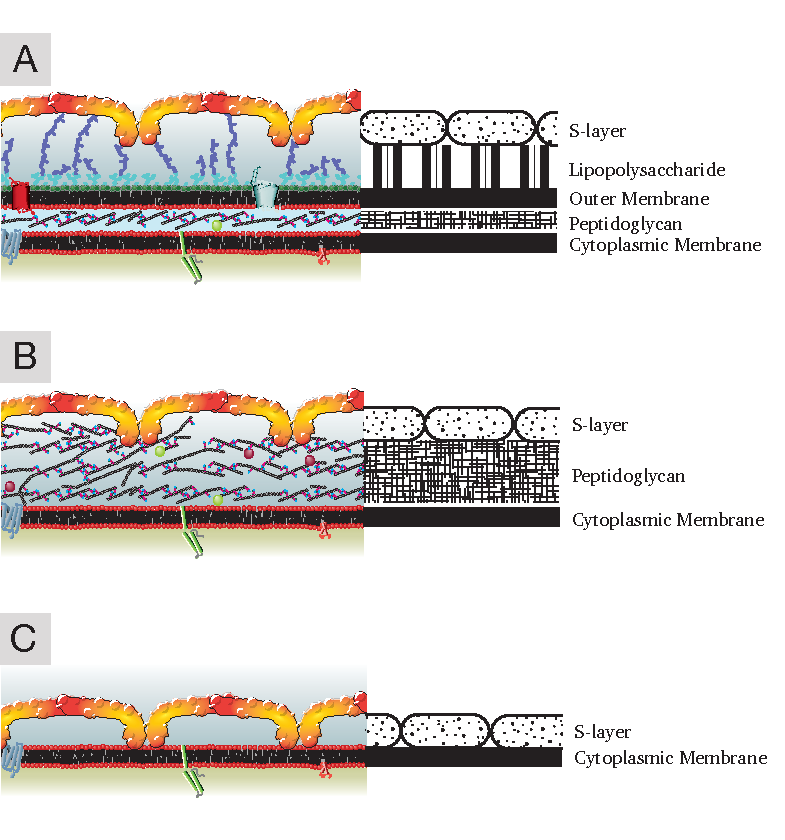
\includegraphics[]{intro/img/celwalls.pdf}
                \end{center}
                \caption[Cross-sectional diagrams of \ac{S-layer} containing cell envelopes]{Cross-sectional diagrams of the cell envelopes of (\textbf{A}) Gram negative bacteria, (\textbf{B}) Gram positive bacteria, and (\textbf{C}) archaebacteria. In all known cases the \ac{S-layer} sits on the extreme outer surface of the cell. (This diagram was inspired by Fig. 1 from \fullcite{sleytr1983crystalline})}
                \label{fig:cellwalls}
        \end{figure}

            Examples of bacteria with oblique \acs{S-layer} are \textit{Bacillus stearothermophilus} NRS2004$/$3a\upcite{messner1986characterization} and \textit{Lactobacillus brevis}\upcite[.]{masuda1980reassembly}
            Examples of bacteria with rectangular \acs{S-layer} are \textit{Corynebacterium diphtheriae}\upcite{kawata1972extracellular} and \textit{Aeromonas salmonicidae} A450\upcite[.]{ishiguro1981loss}
            An example of a bacterium with a triagonal \ac{S-layer} is \textit{Sulfolobus acidocaldarius}\upcite[.]{weiss1974subunit}
            Examples of bacteria with hexagonal \acs{S-layer} are \textit{Bacillus anthracis}\upcite{holt1969comparative} and \textit{Caulobacter crescentus}\upcite[.]{smit1981periodic}

        \begin{figure}[htb] % S-layer symmetries
                \begin{center}
                    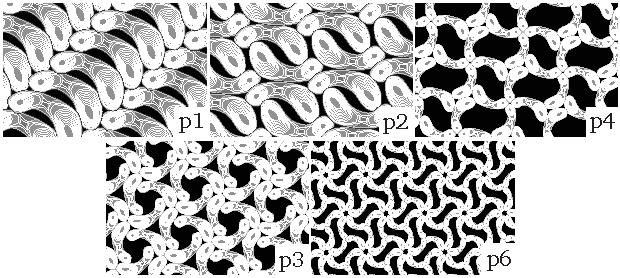
\includegraphics[]{intro/img/symmetries.pdf}
                \end{center}
                \caption[A simple overview of \ac{S-layer} symmetries]{A simple overview of \ac{S-layer} symmetries. p1 and p2 are oblique symmetries. 
                p4 is a rectangular symmetry.  
                p3  is a triagonal symmetry. 
                p6 is a hexagonal symmetry.}
                \label{fig:symmetries}
        \end{figure}


    % subsection s_layer_structure (end)

    \section{History of S-layers} % (fold)
    \label{sec:history_of_s_layers}
       
       % \begin{comment}  % Notes on history
       %      Notes on history of S-layers:
       %          - first seen
       %          - first cloned
       %          - first crystallised

       %      First (always) seen by EM

       %      First seen in Spirillum
       % \end{comment}

        \begin{figure}[p] % First S-layer
                \begin{center}
                    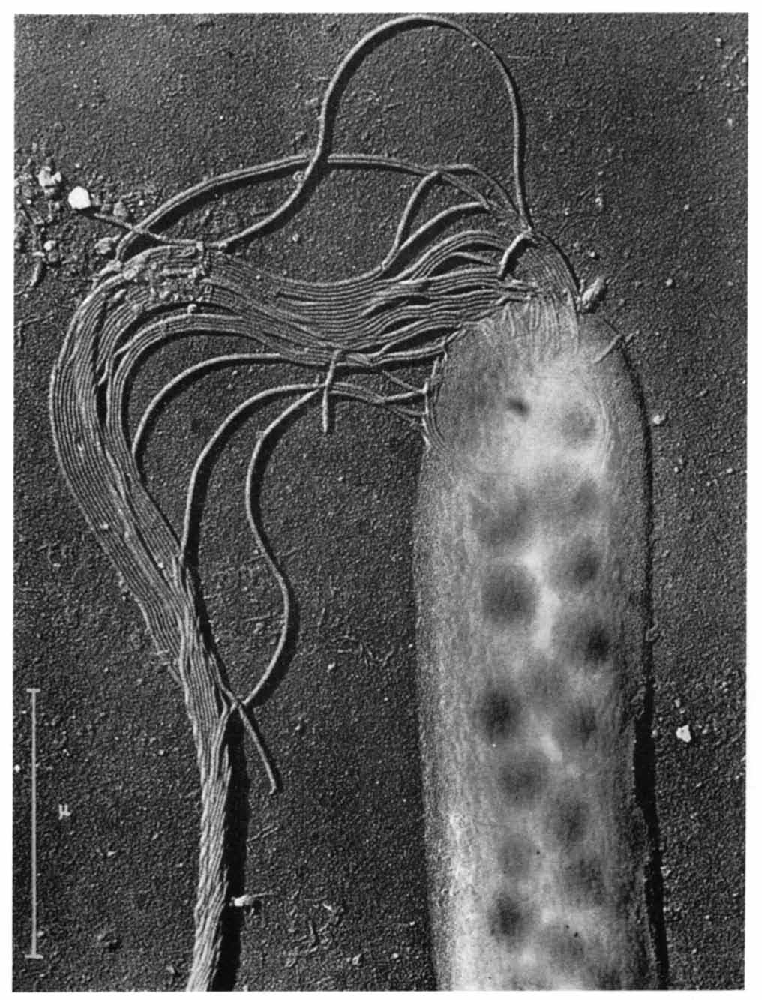
\includegraphics[]{intro/img/firstslayer.pdf}
                \end{center}
                \caption[The first published image of a \ac{S-layer}]{The first published image of a \ac{S-layer}. The hexagonal \ac{S-layer} on the surface of the bacterium --- probably \textit{Spirillum} sp. --- is visible along the edges of the cell body (centre right). The scale bar denotes one micrometre. (This image is Fig. 1 from \fullcite{firstslayer}, reused with full permission from the publisher, Elsevier.)}
                \label{fig:firstslayer}
        \end{figure}
    % section history_of_s_layers (end)
% section paracrystalline_protein_surface_layers (end)

\endinput

Any text after an \endinput is ignored.
You could put scraps here or things in progress.


%    2. Main body
% Generally recommended to put each chapter into a separate file
	%% The following is a directive for TeXShop to indicate the main file %!TEX root = ../MJThesis.tex
\acresetall
\resetlinenumber[1]
{\singlespacing{}
  \chapter{The crystallization and X-ray diffraction of the S-layer protein, RsaA}
\label{ch:crystal}
}
\begin{epigraph}
  \emph{``Please forgive me for presenting, on such a great occasion, results which are still in the making, but the glaring sunlight of certain knowledge is dull and one feels most exhilarated by the twilight and expectancy of the dawn.''} \\---~Max Perutz, 1962 Nobel lecture\\ The father of protein X-ray crystallography.
\end{epigraph}

\section{Introduction} % (fold)
\label{sec:crystal_introduction} 

\lettrine[lines=2]{P}{rotein surface layers} (\acs{S-layer}) are para-crystalline coatings that
surround microbial cells\upcite[.]{beveridge1997v}
 They have various functions, such as adhesion
and immune evasion in pathogenic bacteria\upcite[;]{DallaireDufresne20141, kern2010bsla}
 protection against phage and predation\upcite[;]{koval1991effect, koval1993predation}
 and as a pseudo-membrane in archaea\upcite[.]{Blaurock01101976}
 \acp{S-layer} are composed of either one or a small number of secreted proteins that self assemble
into a contiguous sheet in the extracellular environment. 

Despite their unique features, \acp{S-layer} have not enjoyed the intensive structural
investigations that most other protein families have received, in no
small part due their resistance to 3D-crystallization. The reason why \acp{S-layer} resist
crystallization is not completely understood, but it is definitely related to their proclivity
to self-assemble into large polymeric structures (\ie \acp{S-layer}). We know
that \ac{S-layer} formation plays a role in the crystallization problems because
 the only groups that have successfully crystallized an \ac{S-layer} protein
 have done so by specifically inhibiting or removing the \ac{S-layer} formation ability of
 the proteins\upcite[]{Pavkov20081226, baranova2012sbsb}. It is thought that maybe
 the 2D-\ac{S-layer} formation out competes the 3D-crystallization or maybe the
 2D-\ac{S-layer} structure is incompatible with 3D-crystal growth. Possibly
 there are conditions that exist that would allow for the crystallization of an
 intact \ac{S-layer} protein, but those conditions are currently unknown.

The Gram-negative bacterium \ac{caulobacter} possesses an
\ac{S-layer} that is composed from thousands of copies of a single 98.6 kDa protein, RsaA\upcite[.]{smit1981periodic}
 This particular \ac{S-layer} has been pursued as a potent platform for peptide display and
protein expression\upcite[.]{smit2008heads}
RsaA is secreted from the cell via a type 1
secretion system\upcite[.]{walker94}

 RsaA shares little to no sequence similarity to any
other known protein, except for in the conserved \ac{rtx}
motifs canonically found in all type 1 secreted
proteins\upcite[.]{chenal2009rtx, bingle2000secretion} When the entire RsaA protein
sequence is compared against other proteins with a \ac{blast} analysis the
highest hits returned are unknown proteins from \textit{Skermanella aerolata}
(Score: 1063, Identity: 33.7\%) and \textit{Pseudomonas syringae} (Score: 958,
Identity: 31.5\%). Interestingly, the protein \ac{blast} also returns hits to
the \ac{S-layer} protein from \textit{Campylobacter fetus}, SapA (Score: 598,
Identity: 29.0\%). Closer investigation of the sequence alignment between RsaA
and \textit{C. fetus} SapA shows few extended regions of sequence identity. 
Of the few regions of consistent homology most were \ac{rtx} motifs. There are
no tantalizing clue to be learned from \ac{blast} analysis at this point, but it
may be good platform to translate any future structural information to other
unsolved proteins.

 RsaA further isolates itself in its sequence by featuring a uniquely limited amino
acid composition that is biased towards small, simple residues. This bias
towards  amino acids that are energetically less costly to synthesize is thought to be an evolutionary strategy
for secreted proteins conserved across micobial life and especially in
\ac{caulobacter}\upcite[.]{smith2010economical}

All crystallographic studies of \ac{S-layer} proteins have to inhibit \ac{S-layer} formation. In the
past co-crystallization with nanobodies\upcite[]{baranova2012sbsb}
 and truncation\upcite[]{Pavkov20081226}
 approaches have resulted in monodisperse, crystallizable proteins. Here we describe the
expression of an 804 \ac{aa} C-terminal fragment of RsaA (RsaA \del 0--222) from
its native host, \ac{caulobacter}. The untagged protein was purified
from culture supernate and crystallized by hanging-drop vapor
diffusion. Crystals were grown that diffracted to 2.5 \AA.
Diffraction data were collected at both the \ac{cls} 
and the \ac{ssrl}. RsaA is the first Gram-negative \ac{S-layer} protein to be
crystallized to date.

Crystallization and X-ray diffraction are the two essential first steps of any
crystallization project but the next hurdle of solving the phasing problem is an
equally crucial and fundamental problem in crystallography. Solving the phases
has been the hurdle that this project has stumbled on the most. The unique aspects of
RsaA preclude it from solution through molecular replacement. A multitude of
\ac{MAD} and \ac{SAD} strategies were pursued but without success. The
protein sequence of RsaA was altered through the installation of a decapeptide
sequence, in the hope that it would give the protein better ion-binding
potential for \ac{MAD} phasing, also without success. No solution has solved the problem to date and the atomic structure of RsaA remains undetermined.

\section{Methods}
\label{sec:crystal-materials-and-methods}

\subsection{Strain and plasmid construction}\label{sec:stra-plasm-constr}

\paragraph{Expression strain} The strain used to produce our RsaA truncates was JS4032\upcite[.]{lau2010analysis} 
This strain can also be labeled \caulobacter{} CB2A \textit{$\Delta$sapA $\Delta$manB ::repABC}. The strain's genomic copy of \textit{rsaA} is inactivated by a non-sense frame-shift mutation at the 353$^{rd}$ codon. The gene \textit{sapA} has been removed; it encodes for an S-layer associated protease (SapA) that has been implicated in degrading modified versions of RsaA\upcite[.]{sap} The surface polysaccharides, \ac{EPS}, polyrhamnan, and \ac{OPS}, were all eliminated by disrupting the gene \textit{manB}. \textit{manB} encodes for phosphomannomutase, an important enzyme in the bio-synthesis of many deoxysugars (see \cref{ch:lps} for our investigation on the structure of the \ac{LPS}). Removing these carbohydrate structures causes RsaA to no longer associate with the cell surface and it aids in downstream processing, giving the cells favorable centrifugability. The operon repABC has also been knocked into this strain to allow for the replaction of small broad-host range plasmids that we use for protein expression\upcite[.]{umelo2001development}

\paragraph{Expression vectors} The plasmid used initially in this study, pUC8CVX-RsaA \del{}0--222, was a construct of the plasmid pUC8CVX\upcite[]{nomellini2007s} containing an open-reading frame encoding for the C-terminal 804 AA of RsaA. pUC8CVX, digested with \textit{Bam}HI and \textit{Hin}DIII, was ligated to the 2819 bp fragment from a similarly digested plasmid containing an open-reading frame encoding for RsaA with a \textit{Bam}HI  endonuclease recognition sequence at the 666 bp position created in a previous study\upcite[.]{ford2007s} The plasmid, pUC8CVX-RsaA \del{} 0--222, was then electroporated\upcite[]{gilchrist1991transformation} into the expression strain. The annotated sequence of RsaA is found in the appendix on \cpageref{app:rsaseq}.

The plasmid that was used to produce RsaA \del 0--222 GSCC723, pUC8CVX-RsaA \del{}0--222 GSCC723, was produced by replacing the rear portion of RsaA \del 0--222 in pUC8CVX-RsaA \del 0--222 with a preexisting engineered RsaA fragment. The fragment contained an in-frame insertion of the C-Myc-tag antigen at the 723$^{rd}$ codon\upcite[.]{nomellini2007s} This replacement was done by swapping 2630 bp \textit{Bst}XI--\textit{Hin}DIII fragments. The C-Myc-tag is a decapeptide, \texttt{EQKLISEEDL}, that was derived from the oncogenic human protein Myc, in RsaA we hoped that the added charges would improve the proteins ability to bind useful ions. Our `GSCC' cassette contains the C-myc-tag as well as a few other restriction sites that can be utilized for the instillation of future peptide cassettes, specifically a \textit{Bgl}II site and a \textit{Pst}I site. The translated peptide sequence of the GSCC cassette is \texttt{GSRSVNNASEQKLISEEDLRPSADGS}. 

\subsection{Protein production}
\label{sub:crystal-protein-production}

% I need to have strain stuff here.
Our protein construct, RsaA \del 0--222, was expressed in both a traditional
\ac{ecoli} expression system and in our lab's \ac{caulobacter}
protein expression system\upcite[.]{bingle1997expression, UmeloNjaka20011406, Bingle1990143}
 All attempts to produce protein in \ac{ecoli}
resulted in highly insoluble inclusion bodies.
 Expression levels of RsaA in its native host is notably high\upcite[]{lau2010analysis} but
the system did not initially produce protein in an appropriate form for
crystallization, that is monodisperse, soluble protein. A number of
counter-intuitive methods had to be used to produce a crystallizable form of
RsaA from \caulobacter. The protein encoding gene had to be genetically altered
to produce a truncated form of RsaA, the cells had to be cultured under low
agitation, and the resulting secreted protein had to be concentrated very slowly.

The reasons for an N-terminal truncation of RsaA are two-fold; deletion
of the N-terminus produces protein that no longer anchors itself to
outer membrane, resulting in soluble supernatant protein; and the
N-terminus has been identified as the center of three-fold symmetry, its
deletion should prevent wide-scale \ac{S-layer} formation and aggregation. This is our strategy for preventing \ac{S-layer} formation as discussed in \cref{sec:crystal_introduction}.

% Add something about aggragations
The cells were grown in M16HIGG medium\upcite[]{smitpilin81}
at 30\cel for 72 hours. 250 \millilitre cultures
were used in 2500 \millilitre wide-bottom Fernbach flasks, resulting in shallow
cultures that did not require shaking for sufficient aeration as
agitation of the culture led to macroaggregation of the secreted
protein. We had observed that cells cultured in shaken test tubes produced
aggreagted protein, while cells cultured in rolled test tubes produced soluble
protein.

 The cultures were centrifuged at 6300 rpm in JA-10 bottles for
35 min, the supernates were recovered and recentrifuged. The
supernatants were then filtered through a 0.22 \si{\micro\meter} microfilter to ensure
no cells remained. The protein-containing supernatant was initially
concentrated by lyophilization and rehydration to 1/10 the original
volume. The rehydrated protein solution was dialyzed against distilled
water and microfilitered. Purification was performed over a 26/60 S100
Sephadex size-exclusion chromatography column and mobile phase of 200 \si{\milli\molar} \ce{NaCl} and 10 \si{\milli\molar}
Tris pH 7.5. The first major elution peak was pooled and dialyzed
against distilled water and concentrated by placing the dialysis bags on
\ac{peg} with an average molecular weight of 20 000 Da (Sigma-Aldrich). The protein
solution was slowly concentrated to a final concentration of 3.5--4
\mgperml. Dialysis against \ac{peg} was slow a gentle enough to prevent the
protein from aggregating during concentration. Other methods of concentration,
such as ultrafiltration caused RsaA \del 0--222 to come out of solution.

\begin{figure}[htb]
  	\begin{center}
   		\includegraphics[width=0.8\textwidth{}]{crystal_chapter/img/222purif.pdf}
   	\end{center}
   	\caption[Purification of RsaA \del 0--222 shown by \ac{SDS-PAGE}]{
      The purification of RsaA \del 0--222 as monitored by \ac{SDS-PAGE}.
      \textbf{A}. 7 \microlitre{} of culture supernate of our \caulobacter{}
      expression strain expressing RsaA \del 0--222. \textbf{B}. Each land has
      15 \microlitre{} from separate  size-exclusion chromatography elutions
      from the major peak containing RsaA \del 0--222. The tubes represented by
      these 4 bands were pooled, dialyzed, concentrated, and crystallized.
}
   	\label{fig:222purif}
\end{figure}   

\subsection{Crystallization of RsaA \del 0--222}\label{crystallization}

 RsaA  \del 0--222 was initially crystallized at a concentration of 9 \mgperml. Sparse-matrix screening was performed using the \ac{jcsg} Core I, II, III and IV screens (Qiagen). 
After one week incubation at room temperature, small crystalline shapes were
observed in \ac{jcsg} Core I well 28 (200 \si{\milli\molar}  \ce{MgCl2}, 100 \si{\milli\molar} Tris pH 7, 20\% \ac{peg}
8000). This crystal formation was  not reproducible in the original conditions in
a hanging drop vapor apparatus. Thin plates readily formed once the concentration
of the protein and the \ac{peg} 8000 were both reduced. Thicker, more robust crystals
formed when \ce{MgCl2} was replaced with other Group 2, alkaline earth metal salts, specifically \ce{CaCl2}, \ce{SrCl2}, or \ce{BaCl2}; \ce{SrCl2} was
deemed the most succesful at producing crystals. Final crystallization
conditions were 8.5\% \ac{peg} 8000, 100 \si{\milli\molar} Tris pH 7.4, and 150 \si{\milli\molar} \ce{SrCl2}.
Two crystals forms were observed, planar `plate' crystals and hexegonal
`pencil' crystals. Occasionally the `plate' crystals would grow in clusters where it was advantageous to break off a section of the cluster for diffraction (like the crystal in \cref{fig:crystal-flower}). The `pencil' crystals always formed as individual crystals.

 Mother liquor (\ie the crystallization well solution) amended with 25\% glycerol was used as a cryo-protectant for all
crystals prior to flash freezing in liquid nitrogen or a cryo-nitrogen stream.

\begin{figure}[htb]
  	\begin{center}
   		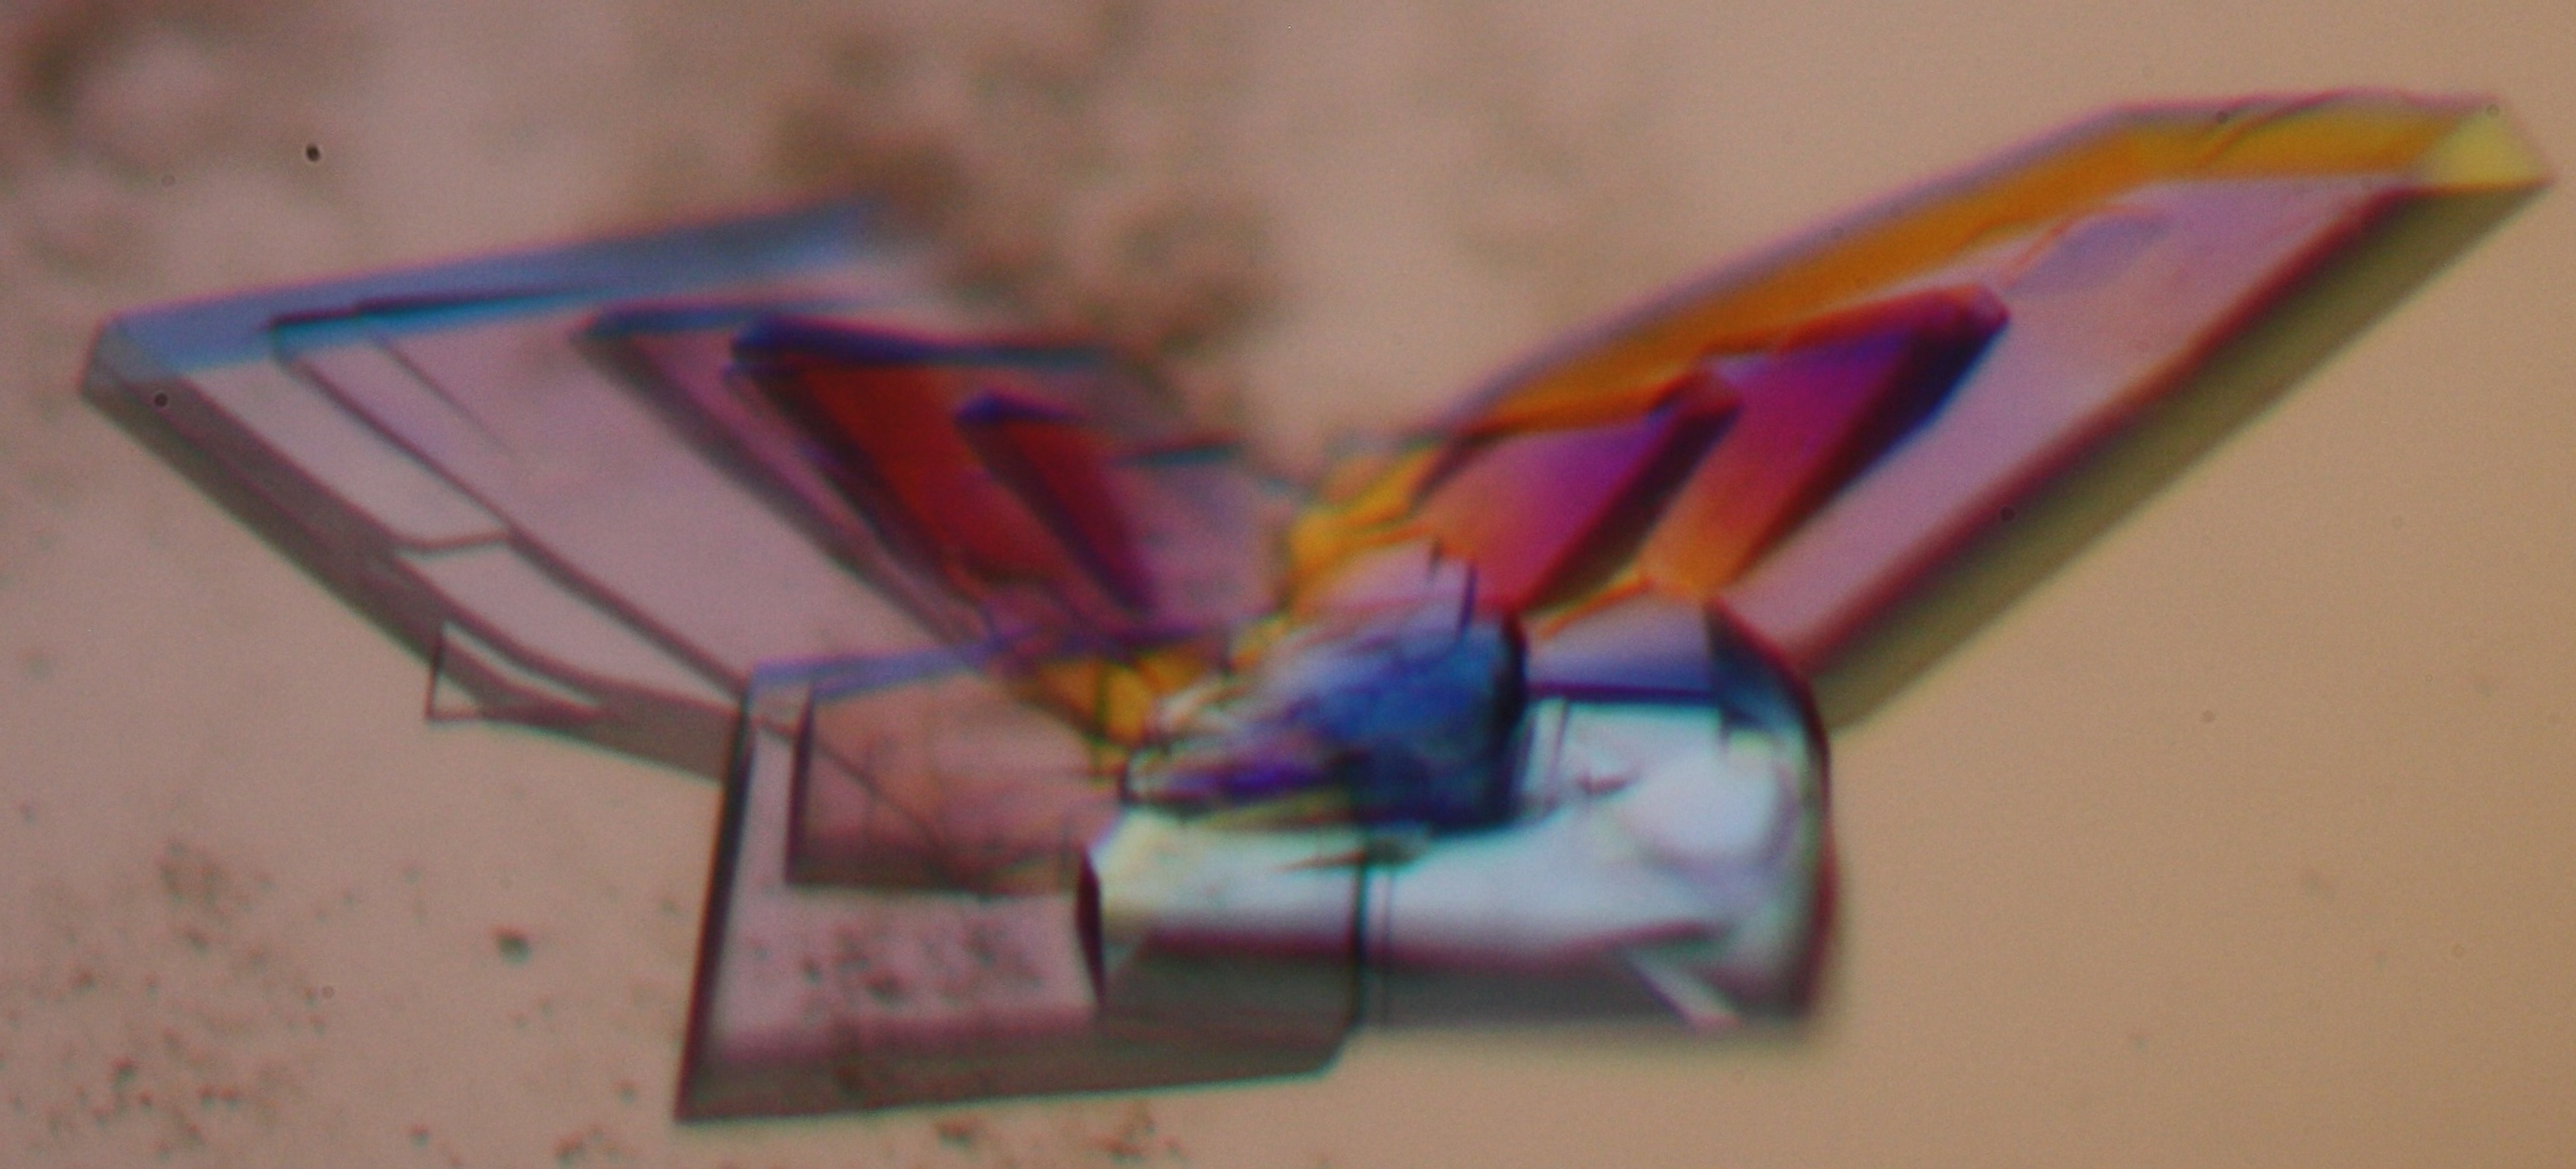
\includegraphics[width=0.7\textwidth]{crystal_chapter/img/bigflowerxtal.jpg}
   	\end{center}
   	\caption[Example of a large cluster of `plate' RsaA \del 0--222 crystals]{An example of a large cluster of `plate' crystals of RsaA \del 0--222. The cluster was just over one millimeter in width from tip to tip. The largest crystal, on the right, was broken off and diffracted using synchotron radiation, resulting in disappointing resolution. The color is imparted by a polarizing filter on the microscope, the crystals are naturally colourless.}
   	\label{fig:crystal-flower}
\end{figure}

\subsection{Crystallization of RsaA \del{}0--222 GSCC723} \label{sec:cryst-rsaa-del0}

RsaA \del 0--222 GSCC723 readily crystallized in the successful conditions used for RsaA \del 0--222. The crystals that formed had a different morphology. The crystals looked dendritic, like trees or snowflakes. Extensive optimizations were performed to improve the shape and size of the crystals but no improved conditions could be found. The final conditions used were 9\% \ac{peg}, 100 \millimolar{} tris pH 7.4, and 150 \millimolar{} \ce{SrCl2}. The protein concentration was 3.5 \mgperml{}, 6 \microlitre{} of protein solution was mixed with 3 \microlitre{} of mother liquor. 

A few of the dendritic crystal clusters had branches that were clean, individual crystals. In those cases, the crystal branches were gently broken off of the main cluster and used for X-ray diffraction.


\subsection{Data Collection Processing}\label{sec:crystal-data-collection}
X-ray diffraction data was collected, multiple times, at two synchotron light
sources: the \ac{cls} in Saskatoon, Saskatchewan and \ac{ssrl} at Stanford
University, California. Both facilities proved suitable for our data collection
needs. The beamlines at \ac{cls} offered a slightly larger spectrum of available
X-ray wavelengths; some of the high energy wavelengths proved useful for
accessing the K-edges of strontium (0.7699 \AA) and bromine (0.9202 \AA). For
our best diffracting crystal, diffraction was performed at the `CMCF 08ID-1'
beamline at \ac{cls}. A wavelength of 1.54 \AA (equal to the copper K-edge) was
used to maximize the overall anomalous signal of iodide.  As
reference, \cref{fig:edges} shows theoretical anomalous scattering coefficients
for most of the elements used in this study. Data were processed using
HKL3000\upcite[]{minor2006hkl} or XDS\upcite[]{kabsch2010xds} ( see
\cref{tab:diffractiondata}); phasing attempts were performed using
Shelx\upcite[]{sheldrick2010experimental} or AutoSol in
Phenix\upcite[.]{adams2010phenix} Data were collected through a full
360$\circ$ of rotation, due the low symmetry found in the `plate' crystals

\begin{figure}[htb]
  	\begin{center}
   		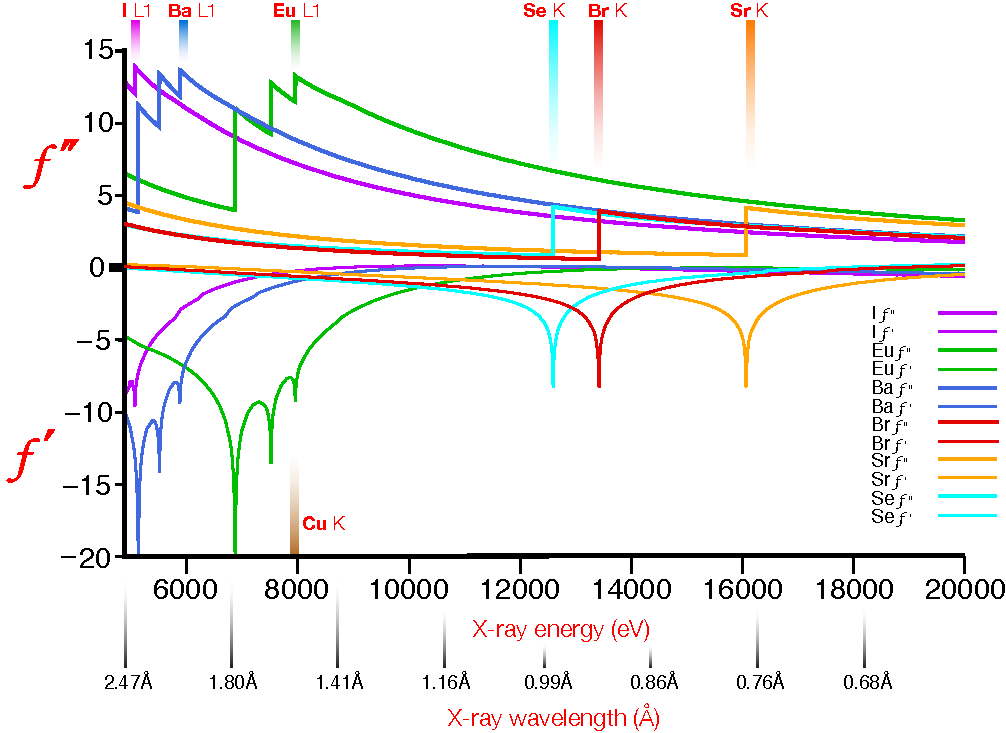
\includegraphics[width=\textwidth]{crystal_chapter/img/edgeplots.pdf}
   	\end{center}
   	\caption[Edge plots for useful anomalous dispersion elements]{
   	Theoretical plots of anomalous scattering coefficients for various elements used in this study. The K-edges and L1-edges that are present within the range of this graph were indicated. Selenium was included because it is often used as a landmark to compare with other elements.}
   	\label{fig:edges}
\end{figure}    

\section{Results}\label{sec:crystal-results}

\subsection{Initial crystallization and optimization}\label{sec:init-cryst-optim} 
 Attempts to crystallize RsaA \del 0--222 started with the pre-assembled crystallization screens \ac{jcsg} Core I, II, III, and IV. Higher protein concentrations were sought because we believed that higher protein concentrations would lead to better results and literature sources recommended protein concentration ranges centering on 10 \mgperml\upcite[.]{jancarik1991sparse} Our protein, RsaA \del 0--222 would readily concentrate to 5--7 \mgperml, but when concentrated beyond 7--9 \mgperml aggregation began to occur, both macroaggregation and microaggregation. Initial screens were assembled at 9 \mgperml, small crystalline shapes were observed after one week at room temperature. Those first crystals grew in JCGS Core I, well 28 with conditions of 20\% \ac{peg} 8000, 200 \millimolar \ce{MgCl2}, and 100 \millimolar Tris pH 7.
 
The first attempts to transfer from a sitting-drop strategy, as used in initial screening, to a hanging-drop strategy, to be used in optimization, were unsuccessful due to widespread protein precipitation/aggregation. Shifting our divalent cation from \ce{Mg^2+} to \ce{Ca^2+} led to small crystals in our drops. Crystals that were grown \ce{Ca^2+} were incredibly thin, but sizable ($>$0.5 \si{\milli\meter}) in the other two dimensions. The biggest improvements came from shifting the cation again to \ce{Sr^2+} and lowering the concentrations of the protein and precipitants. Due to low protein concentrations, larger drop sizes (6--10 \microlitre) were utilized and larger ratios between protein and mother liquor were (1.5:1--3:1) used so that initial conditions would not cause protein precipitation but protein concentrations would eventually get high enough to be supersaturated. Fine tuning of protein concentration and drop ratios were mostly used to optimize nucleations in the drops. RsaA \del 0--222 always nucleated well, leading to more drops full of small crystals than clear drops with no crystals. A protein concentration in the range of 3.5--4.5 \mgperml, mixed in a ratio of 1.5:1 with mother liquor, had the best results, averaging around 3 nucleations per drop. Further optimization to the crystallization conditions, such as lowering salt concentration (200 \millimolar to 150 \millimolar) and raising the pH (7 to 7.4), were of arguable efficacy. 

\subsection{Properties of the RsaA \del 0--222 crystals}\label{sec:properties-crystals}
Our first diffracting crystals RsaA \del 0--222 were `plate' crystals having a rhomboid shape.  \Cref{fig:crystal-panel} shows examples of these rhomboid crystals. The proportional dimensions of the crystals roughly match the relative dimensions of the crystal unit cell (see \Cref{tab:diffractiondata}), although the thickness seemed variable. The crystals grew often as clusters or stacks, which did not aid in diffraction. \Cref{fig:crystal-flower} on \cpageref{fig:crystal-flower} shows one example of how many of these crystal clusters appeared. The rhomboid `plate' crystals were very strong, resisting crushing so well that we were initially worried that they were salt crystals. The `plates' also resisted X-ray induced damage well---often diffracting acceptably after two or three full data collections. 

Later crystallization efforts for RsaA \del 0--222 started to yield crystals that were not rhomboid, they were hexagonal prisms, like `pencils.' Drops identical to and next to drops producing `plate' crystals would often grow `pencil' crystals. A few drops even produced both `plate' crystals and `pencil' crystals. These `pencil' crystals looked like protein crystals under a polarizing filter on the microscope and they were confirmed to be protein by X-ray diffraction. The `pencil' crystals were very fragile and often broke or cracked under gentle manipulation. The `pencils' grew as solitary crystals often on in contact with the lower surface of the crystallization drop. \Cref{fig:pencils} shows a few examples of the hexagonal prism crystals of RsaA \del 0--222.

Low pH solutions would readily crack and destroy any RsaA \del 0--222 crystal. Unfortunately, this pH limitation precluded us from using some soaking agents like uranium compounds and higher concentrations of tantalum bromide. The `plate' crystals were generally more stable in soaking conditions with high salt concentrations than the `pencil' crystals. The `pencil' crystals would quickly crack in high concentrations of \ce{KI} and \ce{KBr}.

\begin{figure}[htb]
  	\begin{center}
   		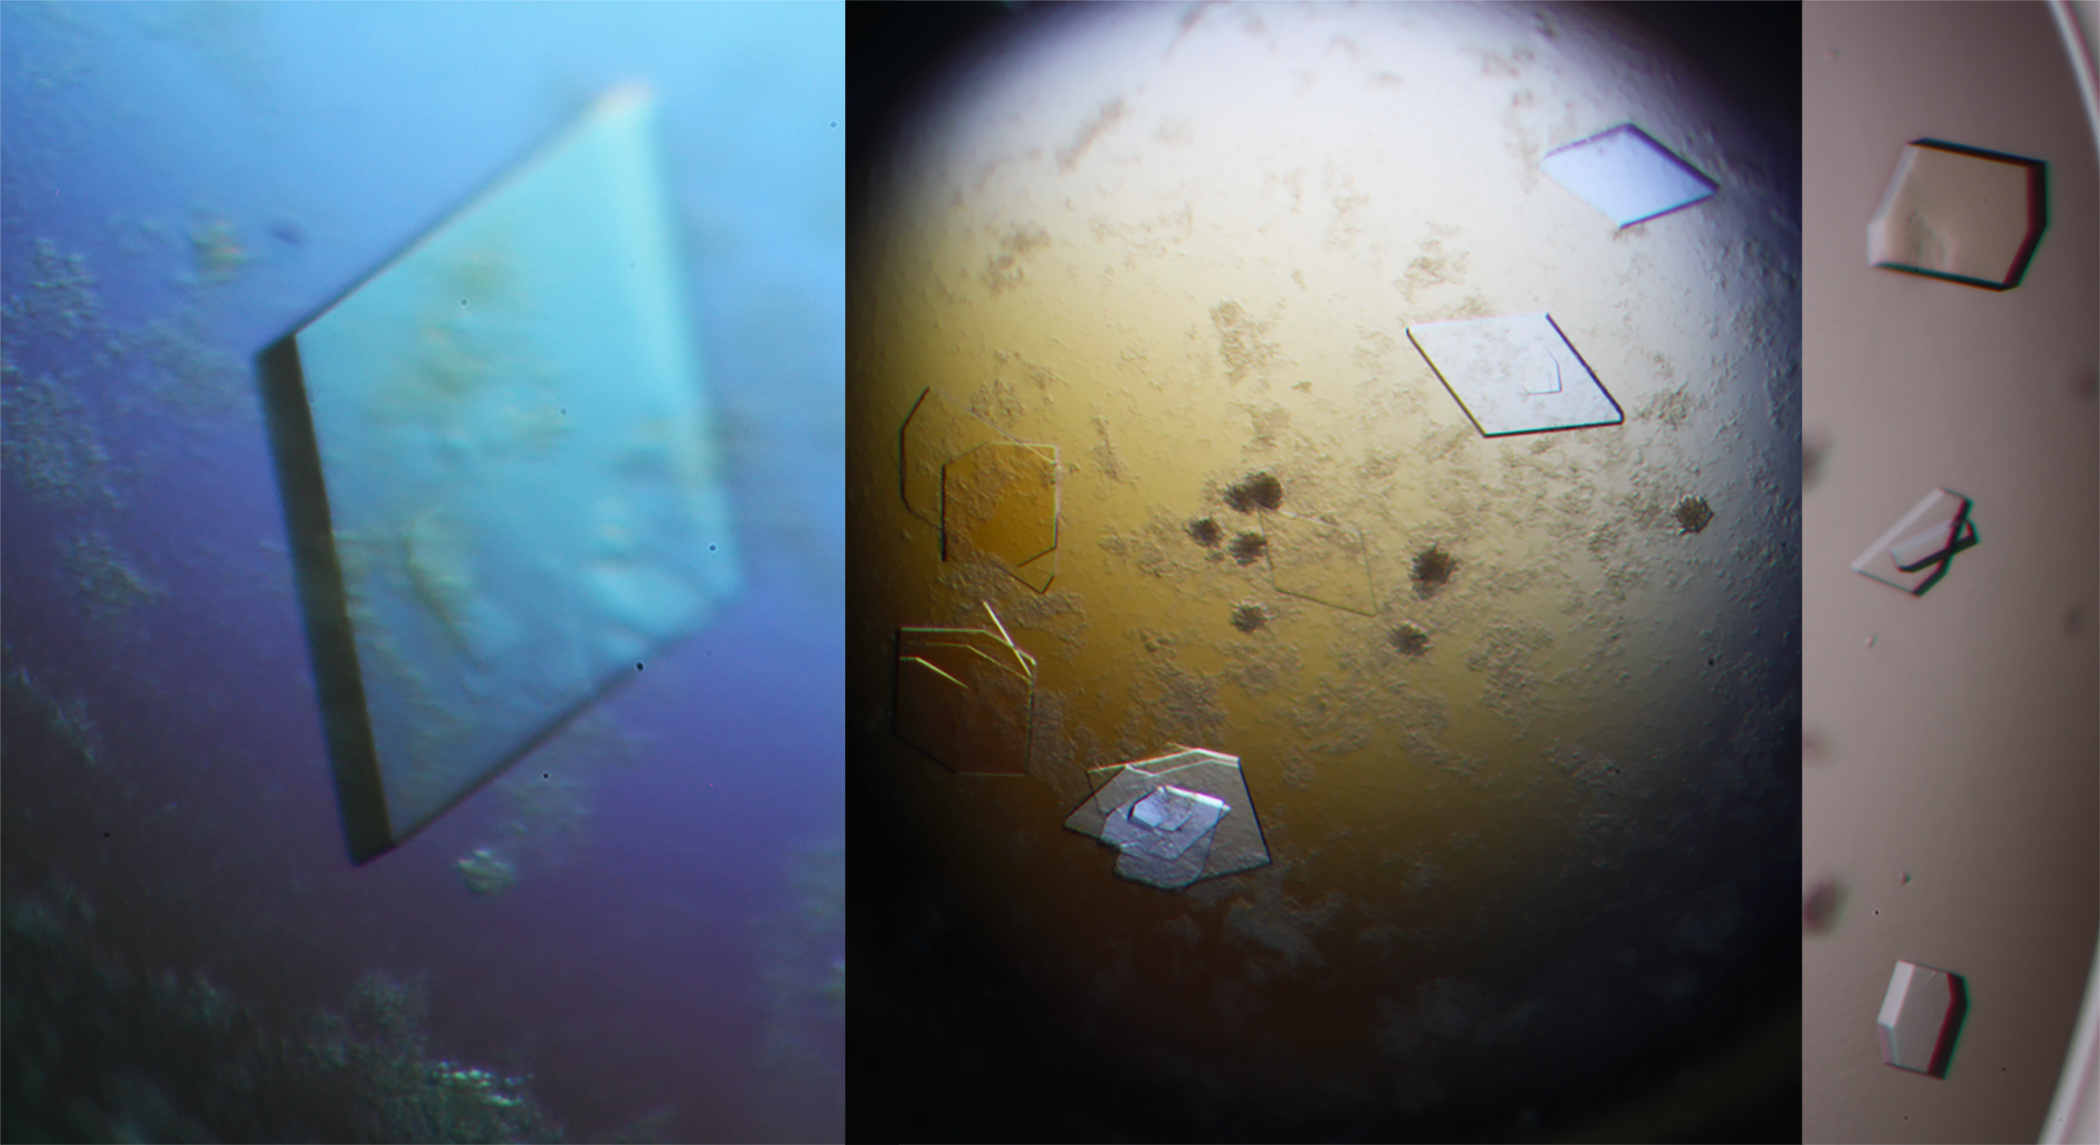
\includegraphics[width=0.9\textwidth]{crystal_chapter/img/goodxtal.jpg}
   	\end{center}
   	\caption[Panel of well diffracting `plate' crystals of RsaA \del 0--222]{A panel of `plate' crystals of RsaA \del 0--222. The left figure show an individual crystal with the common rhomboid shape and relativiley thin width. The center figure shows a wide-view of a drop containing multiple `plate' crystals. The right figure shows three crystals of RsaA \del 0--222 that were grown in the presence of 5 \millimolar{} \ce{EuNO3}. The color in the first two images is imparted by a polarizing filter on the microscope, the crystals are naturally colourless. The colour of the right figure is unadjusted and representative of the natural colour of the crystals.}
   	\label{fig:crystal-panel}
\end{figure}   
\begin{figure}[htb]
  	\begin{center}
   		\includegraphics[width=0.9\textwidth]{crystal_chapter/img/pencils.pdf}
   	\end{center}
   	\caption[A panel of `pencil crystals of RsaA \del 0--222']{A panel of `pencil crystals of RsaA \del 0--222. The left figure shows how some of the `pencils' grew in the presence of `plate' crystals, note the `plates' in that panel were not suitable for X-ray diffraction. The right figure highlights a particularly large `pencil' crystal. These crystals were very fragile.  The color in the images is imparted by a polarizing filter on the microscope, the crystals are naturally colourless.} 
   	\label{fig:pencils}
\end{figure}   

\subsection{Properties of the RsaA \del 0--222 GSCC723 crystals}\label{sec:properties-rsaa-del}
As mentioned before, the only crystals that were formed when using the RsaA \del 0--222 GSCC723 protein were `dendritic' crystals that resembled trees or snowflakes. \Cref{fig:crystal-dendrites} shows a few examples of these crystals. Most of these crystals were too clustered to be used for diffraction but a few of the clusters had branches that could be removed and used for diffraction. \Cref{fig:nice-trees} shows a few of the dendritic clusters that were broken apart and diffracted. 

The RsaA \del 0--222 GSCC723 crystals had similar properties to the RsaA \del 0--222 `plate' crystals; the GSCC723 crystals were very strong and stable in most soaking conditions. Unfortunately due to the poor diffraction, the GSCC crystals' potential ability to bind more phasing ions was never realized.

\begin{figure}[htb]
  	\begin{center}
   		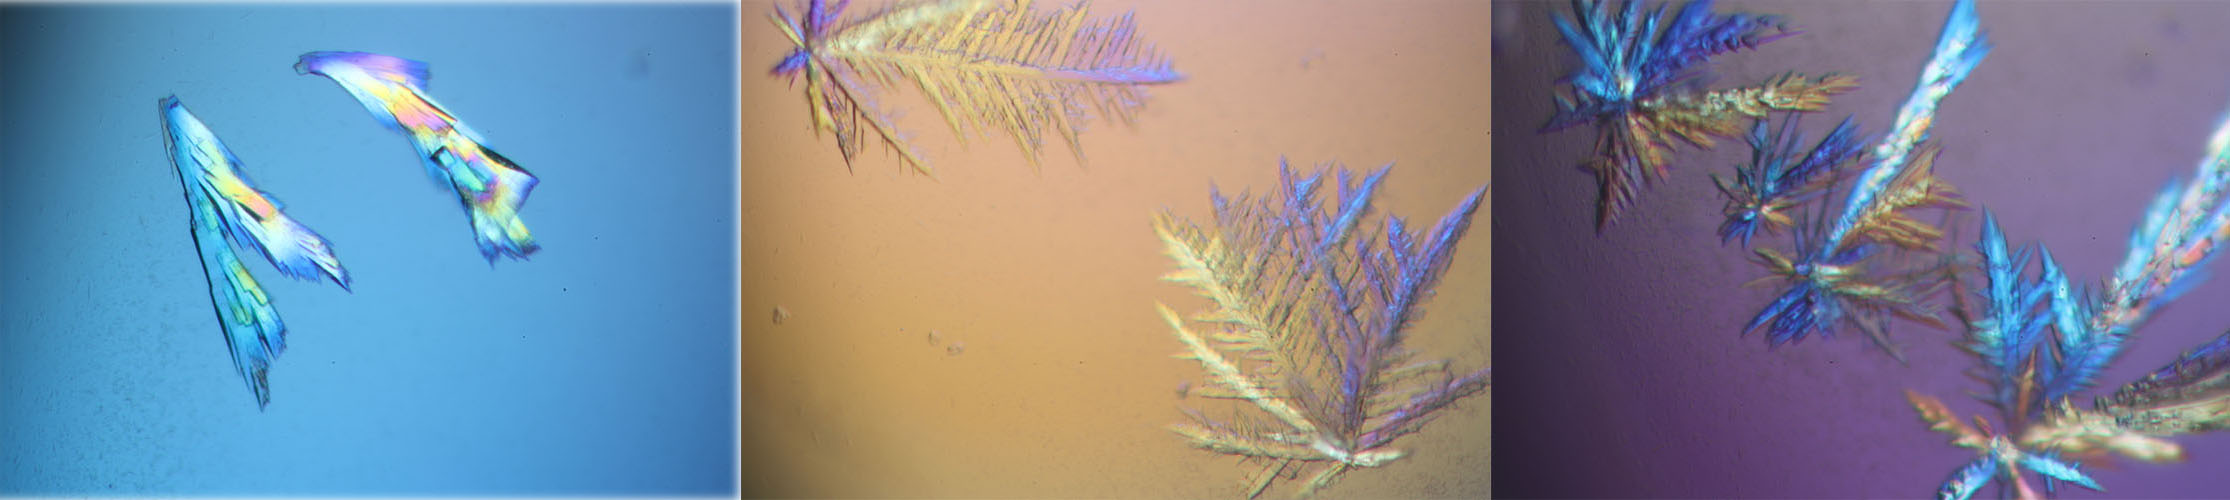
\includegraphics[width=0.9\textwidth]{crystal_chapter/img/dendroXtals.jpg}
   	\end{center}
   	\caption[Examples of unusable `dendritic' RsaA \del 0--222 GSCC723 crystals]{Examples of `dendritic' crystals formed when the RsaA \del 0--222 GSCC723 protein construct was crystallized. The color is imparted by a polarizing filter on the microscope, the crystals are naturally colourless.}
   	\label{fig:crystal-dendrites}
\end{figure}

\begin{figure}[htb]
  	\begin{center}
   		\includegraphics[width=0.9\textwidth]{crystal_chapter/img/nicetrees.pdf}
   	\end{center}
   	\caption[`Dendritic' RsaA \del 0--222 GSCC723 crystals that were used for X-ray diffraction]{A panel of better `dendritic' crystals of RsaA \del 0--222 GSCC723. These are examples of some of the GSCC723 crystals having branches that were suitable for X-ray diffraction. A few of the side crystals were broken off and used for diffraction.  The color in the images is imparted by a polarizing filter on the microscope, the crystals are naturally colourless. The colour of the right figure is unadjusted and representative of the natural colour of the crystals.}
   	\label{fig:nice-trees}
\end{figure}   

\subsection{X-ray diffraction and phasing}\label{sec:x-ray-diffraction}

The biggest issue that we have had to deal with in this crystallography has been the variability of the crystals. The majority of the crystals of RsaA that have been grown have very poor X-ray diffraction. Frustratingly, there was not an effective way to predict which crystal would be  solid performers. Our best results came from a large crystal that was relatively thin---two features that seemed to be important because small crystals did not diffract well and overly thick crystals were plagued with smeared, messy reflections. \Cref{fig:diffraction} shows one frame of data from our best dataset. An interesting aspect of our data, specifically from `plate' and `dendrite' crystals, is the anisotopy we observe in our diffraction. Due to the often poor quality of the data, we would always collect our data through 360$\circ$ which would lead to long collection strategies and increased radiation damage to the crystal. Radiation damage was never too much of an issue though, as the `plate' crystals were incredibly resistant to damage. Table \ref{tab:diffractiondata} gives an overview of our X-ray diffraction data.

        \begin{table}[p]
            \caption[Summary data from our X-ray diffraction of RsaA \del 0--222]{ }
            \begin{center}
                \begin{tabular}{@{}ll@{}}
                    \toprule
										\multicolumn{2}{c}{RsaA \del 0--222}			 \\ \midrule
										Space group				& P2$_{1}$							 \\
										Cell dimensions		&												 \\
										a, b, c (\AA)				& 210.79, 80.74, 221.9	 \\
										$\beta$ ($\circ$)							& 117.46								 \\
										Resolution (\AA)		& 50.00--2.50 (2.54--2.50) \\
										R$_{merge}$				& 0.13 (0.54)						 \\
										I / $\delta$I						 & 13.7 (2.8)							\\
										Completeness (\%) & 99.8 (97.6)						\\
										Redundancy				& 3.8										 \\ \bottomrule
               \end{tabular}
            \end{center}
            \label{tab:diffractiondata}
        \end{table}   
 
 Once we had crystals that diffracted to a suitable extent the final step towards generating an electron density map would be phasing. Molecular replacement strategies failed due to a lack of homologous structures in the Protein Data Bank. The \ac{rtx}  motifs in RsaA provide a tempting region for structural homology, such as the structure in \cref{fig:intro-rtx} (on \cpageref{fig:intro-rtx}). Neither the structures of solved \ac{rtx} motifs as molecular replacement  or the generated Phyre\upcite[]{kelley2015phyre2} structure for RsaA's \ac{rtx} motifs were effective molecular replacement search models. To try and solve the phase problem we turned to the X-ray fluorescence techniques of \ac{MAD} and \ac{SAD}. 

Our main two candidates for \ac{MAD}/\ac{SAD} phasing elements were the halides, iodine and  bromine\upcite[.]{dauter2000novel} These halides were introduced into the crystals by soaking the crystals in \ce{KI} and \ce{KBr}. Iodine does not have an accessible K or L edge but provides a \ac{SAD}  suitable anomalous signal at achievable wavelengths. Refer back to \cref{fig:edges} for the theoretical profiles of anomalous signal. Iodide-soaked `plate' crystals, among the first conditions ever tested, diffracted well and anomalous signal could be detected in their datasets but not enough to allow for densities to be calculated. A great deal of effort went into trying to improve our initial datasets with more of an anomalous component from iodide. Very few subsequent iodide-soaked crystals diffracted at all  and those that did were of low resolution. Bromine has an accessible K$_{a}$ edge at 0.9202 \AA and so it is useful for \ac{MAD}. Unlike iodide, bromide-soaked crystals did not have the high rate of crystals  with no diffraction but like iodide very few bromide-soaked crystals diffracted beyond 4 \AA{}. 

Many other phasing compounds were tested. The lanthanides all provide a strong  anomalous signal and have been successfully used in the past for \ac{SAD}\upcite[.]{baranova2012sbsb} Lanthanum, Lutetium, and Europium were all used as soaking agents but none produced any detectable anomalous dispersion in the resulting datasets. Europium was also successfully used in the mother-liquor of the crystals to be co-crystallized. Unfortuantely, the co-crystallized crystals had no detectable anomalous signal, despite good diffraction. Europium's L$_{1}$ edge is accessible with synchotron radiation (see \cref{fig:edges}), \ac{MAD} fluorescence scans were done to confirm that there was no detectable Europium in the crystals. \Cref{fig:crystal-panel} features a few of the Europium co-crystallized crystals. In the vein of co-crystallization, Strontium and Barium were effective components of the mother liquor, and possibly potent phasing elements, but neither provided an effective solution to the phase problem when tried. More exotic compounds like Tantulum bromide (\ce{Ta6Br12}) and  triiodide were also tried without resulting in the necessary data. 
 
\begin{figure}[htb]
  	\begin{center}
   		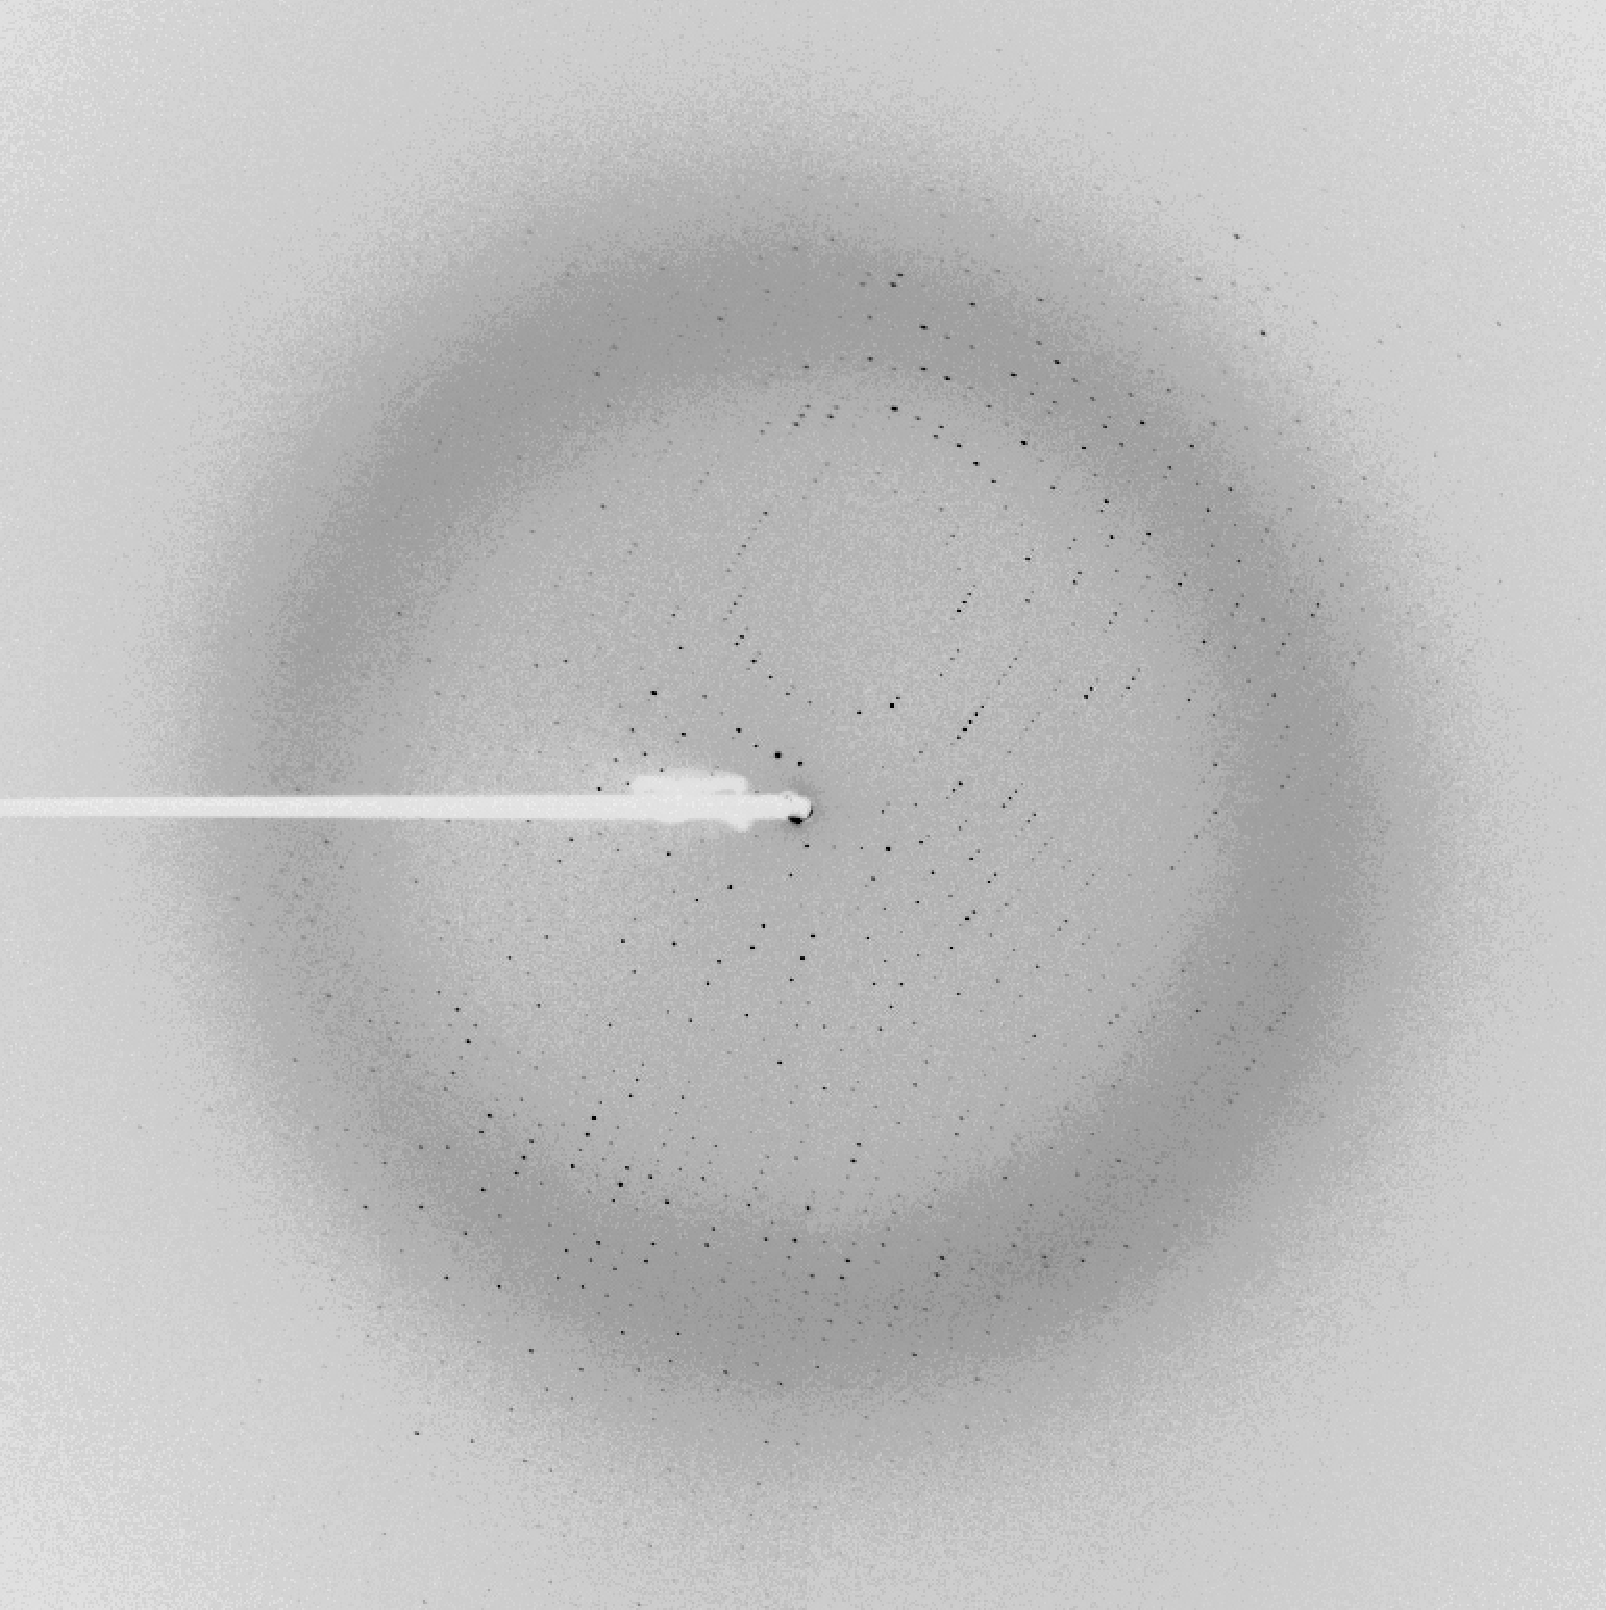
\includegraphics[width=0.9\textwidth]{crystal_chapter/img/rsaadiffraction.pdf}
   	\end{center}
   	\caption[A diffraction pattern of RsaA \del 0--222, `plate' crystal]{This figure shows a frame from a X-ray diffraction data collection. 
This crystal was a large `plate' crystal that was our best diffracting crystal to date. The crystal was soaked in 0.5
 \si{\molar} 
\ce{KI} 
for 30 sec. The wavelength of the incident X-ray beam was set to 1.541 \AA{} (the copper K$_{a}$ edge). Theoretical resolution from this data would have been 2.50 \AA{} if there had been enough anomalous signal to use in \ac{SAD} phasing. Notice the anisotropy in diffraction, \ie the spots reach further from the center to the upper right and lower left.}
   	\label{fig:diffraction}
\end{figure}   

There were only ever a few `dendritic' crystals that were suitable for X-ray diffraction and none of those few diffracted to an extent or in a manner that was conducive to solving the structure of RsaA \del 0--222 GSCC723. One `dendritic' crystal did diffract reliably to 3.5 \AA{} but exhibited multiple overlapping signals, probably due to separate crystals being fused together.  

The `pencil' crystals never diffracted to any significant extent, at most to 6--10 \AA{}. Initial processing of one of the `pencil' diffraction patterns suggested that its space group was P6. A P6 space group has higher symmetry than the P2$_{1}$ space group we observed in our `plate' crystals. We had deep hopes that the higher symmetry would provide better quality data, unfortunately no well performing `pencil' crystals were ever isolated. The only pencil that we did try to perform a complete data collection on quickly lost diffraction due to radiation damage.

\section{Discussion}\label{sec:crystal-discussion}
Our protein construct, RsaA \del 0--222, was expressed our in \caulobacter protein expression system\upcite[.]{bingle1997expression, UmeloNjaka20011406, Bingle1990143} All attempts to produce protein in \ecoli{} resulted in highly insoluble inclusion bodies that resisted refolding (data not shown). Expression levels of RsaA in its native host is notably high\upcite[]{lau2010analysis} but the system did not initially produce protein in an appropriate form. The problem of aggregation persisted in \caulobacter secreted RsaA; the problem was assuaged by the N-terminal deletion construct, RsaA \del 0--222, but was only completely solved when we started to culture the cells without agitation in wide, shallow flasks. Our shallow culture expression system proved successful at producing 130--150 \milligram  of purified, concentrated protein per litre of culture supernate. RsaA is the natural product of \caulobacter but this system could be useful in producing exogenous protein for crystallization by fusion to the required type 1 section signal\upcite[.]{bingle2000secretion}

The reasons for an N-terminal truncation of RsaA are two-fold; deletion of the
N-terminus produces protein that no longer anchors itself to outer membrane,
resulting in free-secreted supernatant protein and the N-terminus has been
identified as the center of three-fold symmetry (Amat et al., 2010). Therefore,
its deletion results in soluble protein that no longer leads to wide-scale
\ac{S-layer} formation or aggregation and is freely secreted into the
supernatant. The success of structurally characterizing any S-layer protein impinges upon overcoming such issues and our strategies resulted in large well-diffracting crystals.

Our `plate' crystals diffracted to 2.5 \AA{} with unit-cell parameters of
a=210.79 \AA, b=80.74 \AA, c=221.9 \AA,  and $\beta$=117.46 degrees. These
crystal unit-cell sizes almost exactly match the 2D unit size of native
\ac{S-layer} repeating unit, a hexamer of RsaA monomers\upcite[.]{smit1992s}
These results suggest that the unit-cell of our crystals is six copies of RsaA
\del 0--222, corresponding to a solvent content of  about 60\%. Our hexagonal
columnar crystals have never diffracted to a suitable resolution, but they are
promising because they have higher symmetry and that may result in improved
datasets. As our protein has no close matches in the structural databases to use
for the purposes of molecular replacement, solving the phase problem was
attempted with iodine derivitization with \ac{SAD} and bromide with \ac{MAD}.
Neither of these approaches gave us the required anomalous data that we would
need for a solution.   RsaA does not have many charged amino-acids, even after
we installed the GSCC cassette, and that is why the halides have been so
strongly pursued; they do not require specific residues for
activity\upcite[.]{dauter2000novel} Patterson analysis of the dataset suggests issues with
pseudotranslational symmetry confounding phasing attempts, with the largest
Patterson peak at a height of about 30\%.  Twinning analyses indicate that no twinning is suspected.

As of writing this, the crystallography portion of this dissertation is still ongoing. We are so close to completing this effort that it is hard to imagine that a solution does not exist. Early successes may have been a curse, leading us down roads that held no promise. The fact is we have developed techniques to crystallize our \ac{S-layer} protein and that is the most important step in this project. To end this chapter, here is a quote from Alexander McPherson's 2004 review on macromolecular crystallography:\upcite[]{mcpherson2004introduction}

\begin{quote}
 Presently, and in the foreseeable future, the only technique that can yield atomic level structural images of biological macromolecules is X-ray diffraction analysis as applied to single crystals. While other methods may produce important structural and dynamic data, for the purposes described above, only X-ray crystallography is adequate. As its name suggests, application of X-ray crystallography is absolutely dependent on crystals of the macromolecule, and not simply crystals, but crystals of sufficient size and quality to permit accurate data collection. The quality of the final structural image is directly determined by the perfection, size, and physical properties of the crystalline specimen, hence the crystal becomes the keystone element of the entire process, and the ultimate determinant of its success.
\end{quote}
	%% The following is a directive for TeXShop to indicate the main file
%!TEX root = ../MJThesis.tex
\acresetall

\chapter{The core and O-polysaccharide structure of the \textit{Caulobacter crescentus} lipopolysaccharide}
\label{ch:lps}
\begin{epigraph}
  \emph{``And so, progressively, the veil behind which Nature has so carefully concealed her secrets
    is being lifted where the carbohydrates are concerned.''} ---~H.\,Emil Fischer, 1902 Nobel
  lecture\\ My great-great-great-great-great-great-great-grand adviser.
\end{epigraph}
\section{Introduction} % (fold)
\label{sec:lps_introduction} 
\lettrine[lines=2]{C}{aulobacter crescentus} (\acs{caulobacter}) is an aquatic alphaproteobacterium
well known for a stalked, crescent cell morphology, asymmetric cell division, and a
\ac{S-layer}. \caulobacter is a widely studied model organism for cell development and
differentiation; despite this, the structure of its \ac{LPS} has not previously been fully
determined.

Interest in the \ac{LPS} of \caulobacter is focused on its immunological
profile\upcite{caulobacterlipida} and its structural role as an anchor for the
self-assembled, para-crystalline \ac{S-layer}\upcite[.]{walker94} The \ac{LPS}
of \caulobacter possesses a much reduced immunogenic activity, most likely due
to its lipid A structure, which is significantly different from that of
\ac{LPS} from enteric bacteria. The lipid A structure has been
reported\upcite[;]{caulobacterlipida} it is a unique molecule containing a
di-diaminoglucose backbone (instead of di-glucosamine) and two galacturonate
moieties that replace the canonical phosphates that are on each end of the
disaccharide in most lipid A molecules. The \caulobacter \ac{S-layer}
non-covalently attaches to the \ac{OPS}\upcite[.]{walker94} However, the
\ac{OPS} structure has not been resolved. Genetic analyses have pointed
towards the unusual N-acetylperosamine being a major
component\upcite[.]{awramgenes} A notable feature of this O-antigen is that it
exists completely hidden beneath the \ac{S-layer}, inaccessible to the
environment\upcite[.]{walker94} Carbohydrate structures from non-pathogenic
bacterial \ac{LPS} are rarely studied and an \ac{LPS} that is sequestered
beneath an \ac{S-layer} is not represented in the literature.
 
In the present study our data has determined the core \ac{OS} structure from
\caulobacter CB15 NA1000 (advancing an earlier report of core
composition\upcite{ravenscroftlps}), as well as the central backbone and
non-reducing ends of its \ac{OPS}. Unexpectedly, we identified a previously
unknown rhamnan polysaccharide. Along with previous reports on lipid
A\upcite{caulobacterlipida} and \ac{EPS}\upcite[,]{ravenscrofteps} we believe
that all the major carbohydrate structures in \caulobacter cell envelope have
now been solved.
% section introduction (end)

\section{Results} % (fold)
\label{sec:lps_results}
	\subsection{Characterization of whole \textsc{lps}} % (fold)
	\label{sub:characterisation_of_whole_lps}
		%% %^Write
  \begin{figure}[htb]
    \begin{center}
      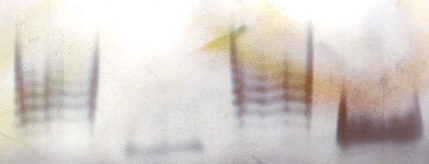
\includegraphics[width=0.3\textwidth]{lps_chapter/img/lpssilverstain.jpg}
    \end{center}
    \caption[Visual comparison of \ecoli O122 \ac{LPS} and \caulobacter \ac{LPS}]{Visual comparison
      of silver stained \ecoli O122 \ac{LPS} and \caulobacter \ac{LPS}. \ac{LPS} samples were run on
      a \ac{SDS-PAGE} and silver stained. Lanes 1 and 3 contain equal amounts of \ac{LPS} from
      \ecoli O122. Lanes 2 and 4 contain our isolated \ac{LPS} from \caulobacter. Lane 4 has twice
      the loaded amount compared to lane 2 to demonstrate that there are no minor, hidden
      bands. Notice the canonical `laddering' pattern of \ecoli\ \ac{LPS} and the distinctly
      singular band of \caulobacter\ \ac{LPS}.}
    \label{fig:lpssilverstain}
  \end{figure}

  \begin{figure}[htp]
    \begin{center}
      \includegraphics[]{lps_chapter/img/lpsvisuals.pdf}
    \end{center}
    \caption[Four different visualisations of \caulobacter\ \ac{LPS}]{Four different visualisations
      of \caulobacter\ \ac{LPS}. \textbf{A}. Western blot with rabbit anti-\ac{OPS} serum used as
      the primary probe. \textbf{B}. Far-western blot with RsaA \del 277--784 used as the primary
      probe and rabbit anti-RsaA serum used as the secondary probe. \textbf{C.} Schiff stained
      \ac{SDS-PAGE}. \textbf{D}. Silver stained \ac{SDS-PAGE}. The smooth-\ac{LPS} (\ie containing a
      complete \ac{OPS}) runs as a single band at roughly the equivalent rate of a 50 kDa protein
      and is visible in all lanes. The faint band visible at 30 kDa in the western blot (A) is of
      unknown source. The faint 30 kDa band is not seen in by far western (B), Schiff stain (C), or
      silver stain (D).}
    \label{fig:lpsvisuals}
  \end{figure}

  \begin{figure}[htb]
    \begin{center}
      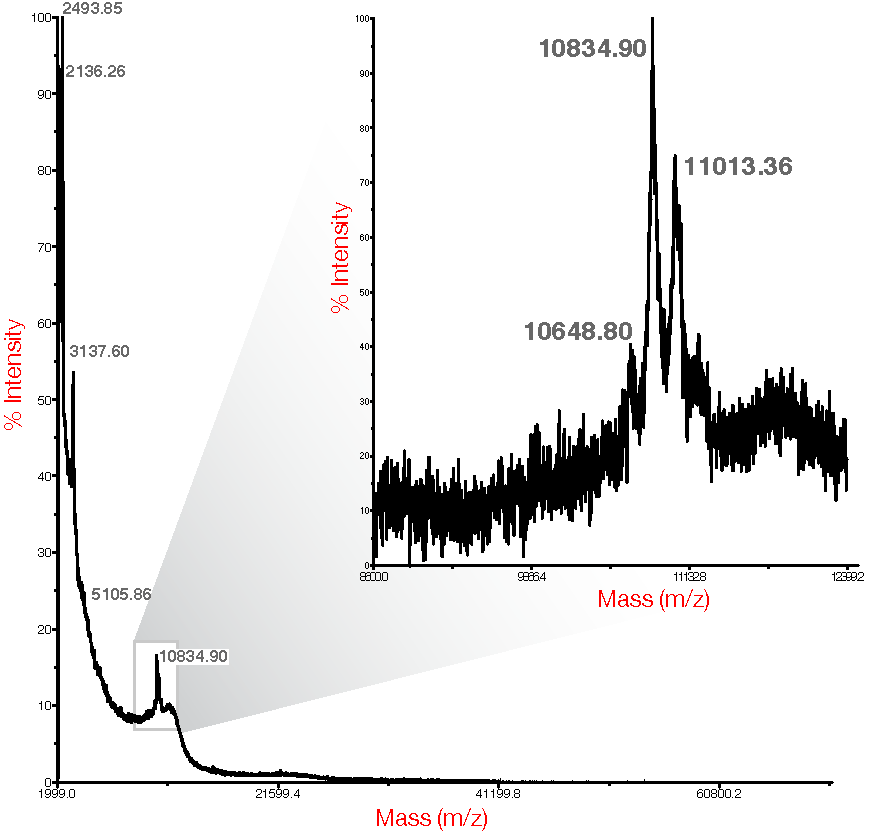
\includegraphics[]{lps_chapter/img/malditof.pdf}
    \end{center}
    \caption[\Ac{MALDI-TOF} analysis of intact, whole \ac{LPS} from \caulobacter]{\ac{MALDI-TOF}
      analysis of intact, whole \ac{LPS} from \caulobacter. The insert highlights the peaks
      attributed to \ac{LPS}. The major \ac{LPS} peak is labelled 10834.90 m/z}
    \label{fig:lpsmalditof}
  \end{figure}
	% subsection characterisation_of_whole_lps (end)

	\subsection{Initial assessment and component analysis} % (fold)
	\label{sub:initial_assessment_and_component_analysis}

  The \ac{PS} was released from the \ac{LPS} by hydrolysis with acetic acid. \textsuperscript{1}H
  \ac{NMR} spectrum of the \ac{PS} (\cref{fig:lpsfig1})) contained a large number of partially
  overlapping signals of various intensities in the anomeric region. It was obviously not a regular
  polymer with well-defined repeating units. Attempts to separate this material by anion-exchange
  chromatography led to the isolation of a number of fractions from neutral to slightly retained,
  but all of them had virtually identical \ac{NMR} spectra. Methylation of the polysaccharide led to
  the identification of 3- and 3,4-substituted mannopyranose, terminal glucopyranose (derived from
  side-chain 3-O-MeGlc), terminal, 3-, 4-, and 2,4-substituted rhamnopyranose, 3-substituted PerNAc,
  and an unidentified derivative resembling methylated PerN that eluted between dimethylhexose
  derivatives and 3-substituted PerNAc. To identify the position of the methyl groups in naturally
  methylated monosaccharides, methylation was conducted with \ce{CD3I}. This confirmed the
  identification of tetramethylglucitol as originating from 3-O-MeGlc, but did not identify any
  other naturally methylated monosaccharides, visible in \ac{NMR} spectra. An unknown derivative
  received two deuterated methyl groups.

  \begin{figure}[ph] %% 1D NMR Spectra
    \begin{center}
      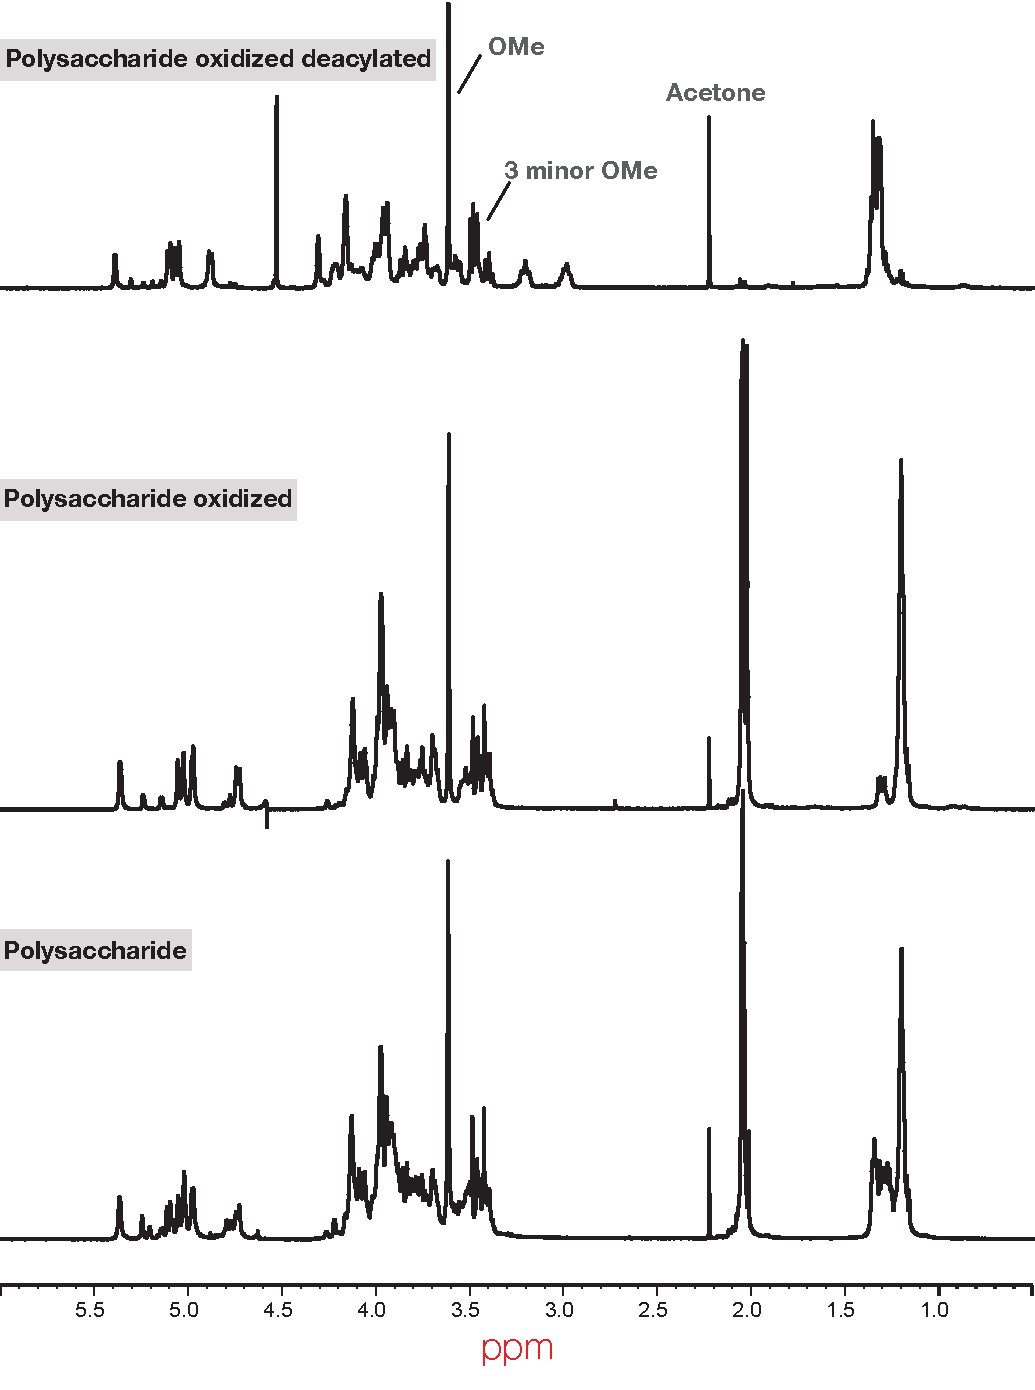
\includegraphics[height=0.9\textheight]{lps_chapter/img/lpsfig1.pdf}
    \end{center}
    \caption[\textsuperscript{1}H \ac{NMR} spectra of \caulobacter{} \ac{OPS}]{\textsuperscript{1}H
      \ac{NMR} spectra of the intact \caulobacter{} \ac{OPS} (bottom trace), double oxidized
      polysaccharide (middle trace) and N-deacylated double oxidized polysaccharide (upper trace).}
    \label{fig:lpsfig1}
  \end{figure}
	% subsection initial_assessment_and_component_analysis (end)

  \subsection{Identification of similar glycan structures by RsaA binidng} \label{sec:ident-simil-glyc}
  
  A service available at \ac{cfg} Core H at Emory University is glycan array screening\upcite[.]{blixt2004printed, alvarez2006identification} Fluorescently labeled lectins can be screened over an microarray of 465 known glycan structures commonly found in mammals. The array can be used to identify targets of known carbohydrate-binding proteins, such as RsaA. We hoped that RsaA may bind a glycan on the array and that the structure of that carbohydrate may inform us on the structure of the \ac{OPS} from \caulobacter. Due to our initial component analysis, knew that our \ac{OPS} differed significantly from any of the glycans in the array, at least compositionally (\vpageref{sub:initial_assessment_and_component_analysis}). RsaA (specifically RsaA \del 277--784) was found to not measurably bind any of the glycan structures found on the array. 

	\subsection{O-antigen structure determination (\textsc{ps}1)} % (fold)
	\label{sub:o_antigen_structure_determination_ps1_}

  A set of 2D spectra [\ac{gCOSY}, \ac{TOCSY}, \ac{NOESY},
  \textsuperscript{1}H-\textsuperscript{13}C \ac{gHSQC}, \ac{gHMBC}] was obtained for the
  \ac{PS}. There were many (more than 20) lines of correlations from the anomeric signals. Later,
  after the analysis of \ac{PS} degradation products, most of them could be assigned to particular
  structures (\cref{fig:lpsops,fig:lpsends,fig:lpsrhamnan}). Polysaccharide heterogeneity was not
  caused by random acetylation, but \ac{PS} contained 4 methyl groups (one major and 3
  minor). Monosaccharide analysis revealed L-Rha, D-Man, D-PerN (perosamine, 4-aminodeoxyrhamnose),
  and 3-O-MeGlc. Other methylated monosaccharides were not identified by \ac{GC-MS} as alditol
  acetates, possibly due to low content or degradation during hydrolysis. The \ac{GC-MS} data is
  presented in \cref{fig:monosaccharide_analysis}.

  \begin{figure}[htb] %% monosaccharides
    \begin{center}
      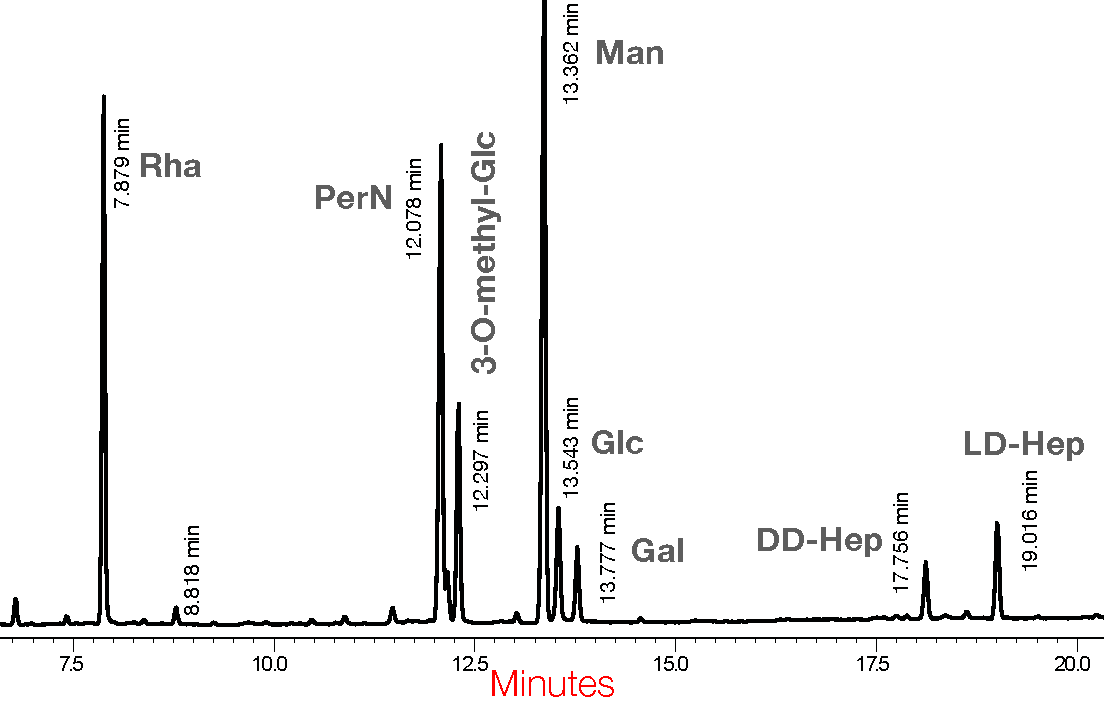
\includegraphics[width=\textwidth]{lps_chapter/img/lps_monosaccharides.pdf}
    \end{center}
    \caption[Monosaccharide analysis of \ac{LPS}]{Monosaccharide analysis of \caulobacter\
      \ac{LPS}. Alditol acetates derivatives of the \ac{LPS} component monosaccharides were
      separated and identified by \ac{GC-MS}. The protocol used is described on
      \cpageref{sub:monosaccharide_analysis}.}
    \label{fig:monosaccharide_analysis}
  \end{figure}

		In an attempt to simplify the structure, \ac{PS} was oxidized with \ce{NaIO4}, reduced with
    \ce{NaBD4}, hydrolysed with 2\% \ce{AcOH}, and the products were separated on a Biogel P6 column
    to give a polymer and an \ac{OS}, \ac{OS}1. Analysis of \ac{OS}1 will be described below. For
    some reason not all of the rhamnan was oxidized, and some of its signals persisted in the
    spectra of the remaining polymer (without side-chain Rha F). To remove the rest of it, the
    oxidation was repeated to produce \ac{PS}1. Spectra still contained some signals of minor
    components, analysed later. Assignment of the spectra of the non-oxidisable polymer \ac{PS}1 was
    difficult due to complete or partial overlap of the H-2,3,4,5 signals of PerNAc. To improve
    signal spread, \ac{PS}1 was deacylated with 4 M \ce{NaOH}. At this point the major polymer
    became positively charged and an attempt was made to separate it from the minor components using
    cation-exchange chromatography. However, all material was eluted together at high salt
    concentration, thus indicating that all components were chemically bound together. Assignment of
    the spectra (\cref{fig:lps2dnmr}, \cref{tbl:lpsops}) became possible at this stage due to better
    signal spread (H-4 signals of PerN moved to high field due to deacylation) and the sequence
    shown on \cref{fig:lpsops} was proposed. Spectra contained the signals of two
    $\beta$-mannopyranose, $\alpha$-3-O-MeGlc, and two -Per4N. The following interresidual \ac{NOE}
    and \ac{HMBC} correlations were used to determine the sequence: R1:L3, L1:Z3, Z1:Q3, Q1:W3,
    W1:X3, A1:X4. \Ac{PS}1 had trisaccharide repeating units composed of $\beta$-mannose and two
    $\alpha$-PerNAc residues, and every second repeating unit carried a side branch of 3-O-MeGlc. It
    seems that side-chains were present quite regularly at each second trisaccharide repeat of the
    main chain, because \ac{NOE} correlations were observed between the repeating units with and
    without 3-O-MeGlc, and not between units of the same structure. Thus altogether, the repeating
    unit contained seven monosaccharides.

		\begin{figure}[H]
			\begin{center}
				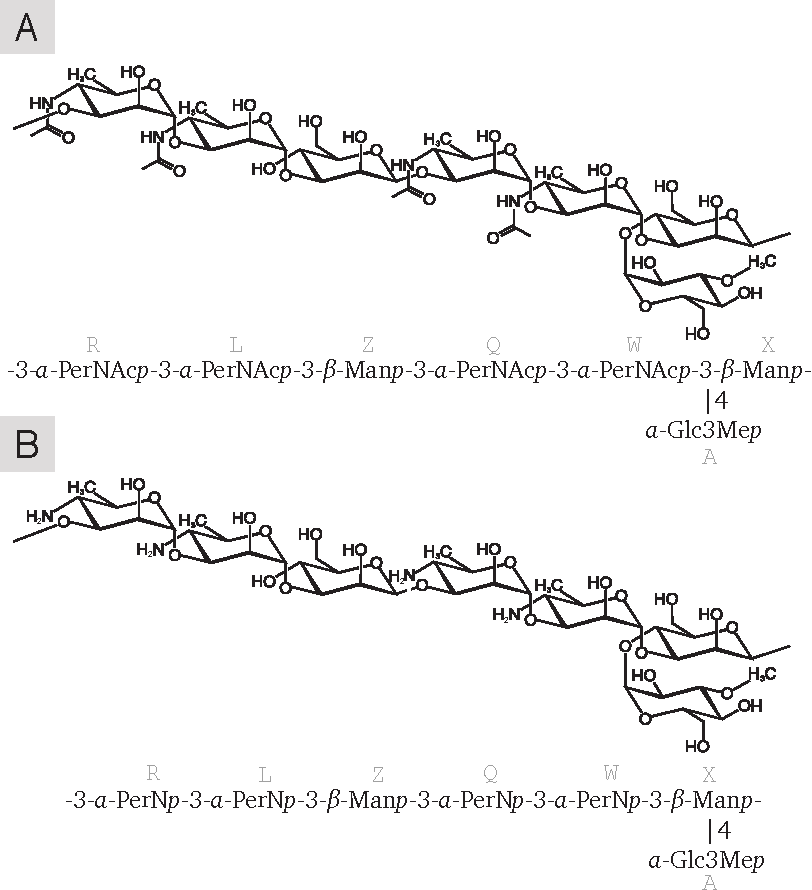
\includegraphics[]{lps_chapter/img/lpsops.pdf}
			\end{center}
			\caption[The structure of the \caulobacter \ac{OPS}]{The structure
            of the \caulobacter \ac{OPS}. \textbf{A.} The intact repeating unit,
            \ac{PS}1. \textbf{B.} The deacylated product of \ac{PS}1.}
			\label{fig:lpsops}
		\end{figure}

		\begin{figure}[H]
			\begin{center}
				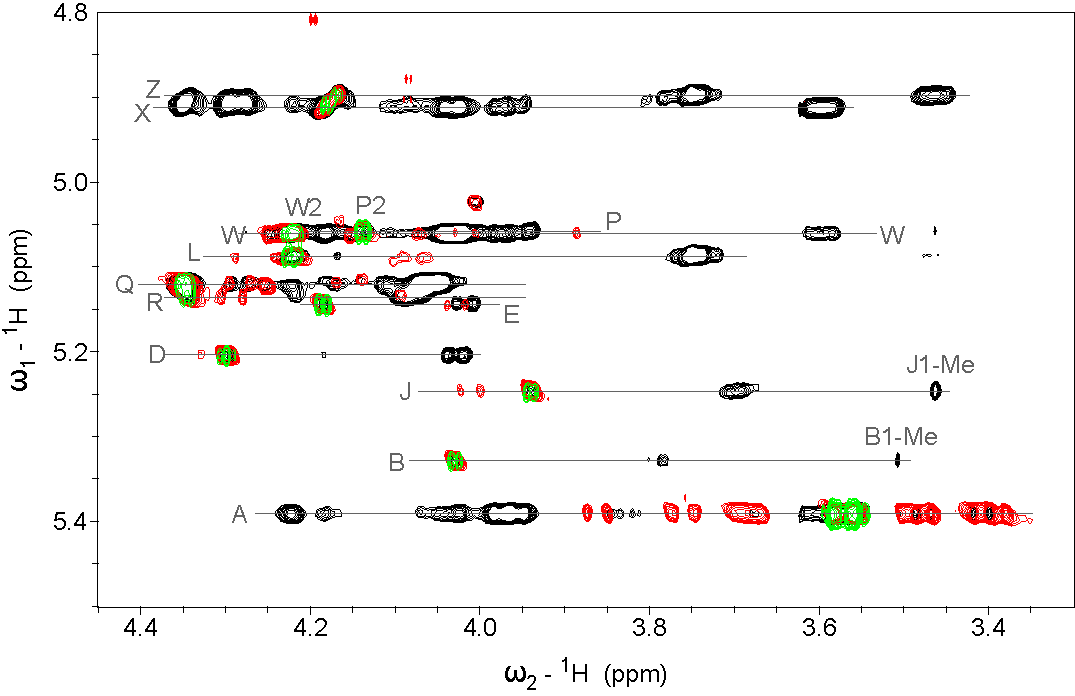
\includegraphics[width=0.9\textwidth]{lps_chapter/img/lpsfig3.pdf}
			\end{center}
			\caption[2D \ac{NMR} of \caulobacter{} \ac{PS}1]{Overlap of \ac{COSY} (green), \ac{TOCSY}
        (red) and \ac{ROESY} (black) correlations from anomeric protons of double oxidized
        deacylated \caulobacter{} \ac{PS}1.}
			\label{fig:lps2dnmr}
		\end{figure}
		\begin{table}[hp] % LPS OPS
			\centering
			\caption[\Ac{NMR} data for \caulobacter \ac{PS}1]{\Ac{NMR} data for \caulobacter \ac{PS}1 (40\cel) and deacylated \ac{PS}1 (50\cel). Me at 3.62/61.3 ppm.}
			\label{tbl:lpsops}
			\begin{tabular}{@{}rccccccc@{}}
				\toprule
				\multicolumn{8}{c}{PS1} \\ \midrule
     &   & 1     & 2    & 3    & 4    & 5    & 6 \\ \midrule
				\multirow{2}{*}{PerNAc R}      & H & 4.97  & 3.98 & 4.13 & 3.92 & 3.91 & 1.21 \\
     & C & 103.3 & 68.2 & 75.5 & 52.4 & 69.4 & 18.0 \\
				\multirow{2}{*}{PerNAc Q}      & H & 4.98  & 3.97 & 4.11 & 3.92 & 3.91 & 1.21 \\
     & C & 103.3 & 68.2 & 75.5 & 52.4 & 69.4 & 18.0 \\
				\multirow{2}{*}{PerNAc L}      & H & 5.05  & 4.12 & 3.99 & 3.98 & 3.98 & 1.21 \\
     & C & 103.3 & 70.4 & 78.2 & 53.0 & 69.4 & 18.0 \\
				\multirow{2}{*}{PerNAc W}      & H & 5.02  & 4.12 & 3.96 & 3.98 & 3.98 & 1.21 \\
     & C & 104.0 & 70.4 & 77.8 & 53.0 & 69.4 & 18.0 \\
				\multirow{2}{*}{$\beta$-Man X} & H & 4.74  & 4.09 & 3.98 & 3.90 & 3.54 & 3.80; 3.96 \\
     & C & 97.8  & 72.1 & 85.4 & 72.1 & 75.8 & 62.6 \\
				\multirow{2}{*}{$\beta$-Man Z} & H & 4.72  & 4.06 & 3.70 & 3.68 & 3.41 & 3.77; 3.96 \\
     & C & 98.2  & 71.9 & 82.3 & 67.2 & 77.3 & 62.4 \\
				\multirow{2}{*}{Glc3Me A}      & H & 5.36  & 3.51 & 3.40 & 3.44 & 3.68 & 3.75; 3.85 \\
     & C & 100.0 & 72.2 & 84.1 & 70.1 & 74.1 & 61.6 \\ \midrule
				\multicolumn{8}{c}{Deacylated PS1} \\ \midrule
				\multirow{2}{*}{PerN R}        & H & 5.13  & 4.34 & 4.29 & 3.30 & 4.18 & 1.38 \\
     & C & 103.5 & 67.4 & 75.0 & 53.4 & 67.8 & 18.0 \\
				\multirow{2}{*}{PerN Q}        & H & 5.11  & 4.34 & 4.29 & 3.30 & 4.18 & 1.38 \\
     & C & 103.5 & 67.4 & 75.0 & 53.4 & 67.8 & 18.0 \\
				\multirow{2}{*}{PerN L}        & H & 5.08  & 4.22 & 4.06 & 3.11 & 4.09 & 1.35 \\
     & C & 103.9 & 69.9 & 79.9 & 53.6 & 69.5 & 18.0 \\
				\multirow{2}{*}{PerN W}        & H & 5.06  & 4.22 & 4.06 & 3.11 & 4.09 & 1.35 \\
     & C & 103.9 & 69.9 & 79.9 & 53.6 & 69.5 & 18.0 \\
				\multirow{2}{*}{$\beta$-Man X} & H & 4.91  & 4.18 & 4.03 & 3.96 & 3.59 & 3.83; 3.96 \\
     & C & 98.0  & 71.7 & 85.0 & 71.7 & 75.9 & 62.1 \\
				\multirow{2}{*}{$\beta$-Man Z} & H & 4.90  & 4.18 & 3.75 & 3.75 & 3.46 & 3.83; 3.96 \\
     & C & 98.0  & 71.7 & 82.0 & 67.0 & 77.4 & 62.1 \\
				\multirow{2}{*}{Glc3Me A}      & H & 5.39  & 3.57 & 3.40 & 3.48 & 3.68 & 3.76; 3.86 \\
     & C & 100.2 & 72.2 & 84.0 & 70.0 & 74.1 & 61.7 \\ \bottomrule
			\end{tabular}
		\end{table}
	% subsection o_antigen_structure_determination_ps1_ (end)
  
	\subsection{Minor component determination} % (fold)
	\label{sub:minor_component_determination}

  \ac{PS} and \ac{PS}1 spectra contained signals of minor components, which could not be removed by
  chromatography, as described above. They probably represented the non-reducing ends of the major
  chain, \ac{PS}1 (\cref{fig:lpsends}). The minor components contained methylated Rha (2-O-Me-Rha
  residue J and 2,3-Me$_2$-PerN residue B). The position of the methyl groups were found from
  \ac{HMBC} correlations between protons of methyl groups and carbon atoms bearing OMe groups, which
  all were well visible and did not overlap with other signals due to their low field
  position. Thus, two independent structural fragments, 1 and 2, were found and are shown in
  \cref{fig:lpsends}. Mannose residues Z' and Z" at the non-reducing ends of these fragments were
  further linked to PerN residues, indistinguishable from the PerN of the main chain. PerN residue D
  had upfield shifted C-2 and downfield shifted C-3 signals (\cref{tbl:lpsends})), which have not
  been explained. It appears that its O-3 was phosphorylated, producing typical phosphorylation
  signal shifts and broadening of the H-3 signal, but \textsuperscript{1}H-\textsuperscript{31}P
  \ac{HMQC} \ac{NMR} spectrum showed no signals, possibly due to the low abundance of this
  residue. Possibly Rha residues inserted in the structure resembling \ac{PS}1 represented the
  attachment point of the rhamnan (\ac{PS}2) to \ac{PS}1, if they were linked together.

		 \begin{figure}[htb]
		 	\begin{center}
		 		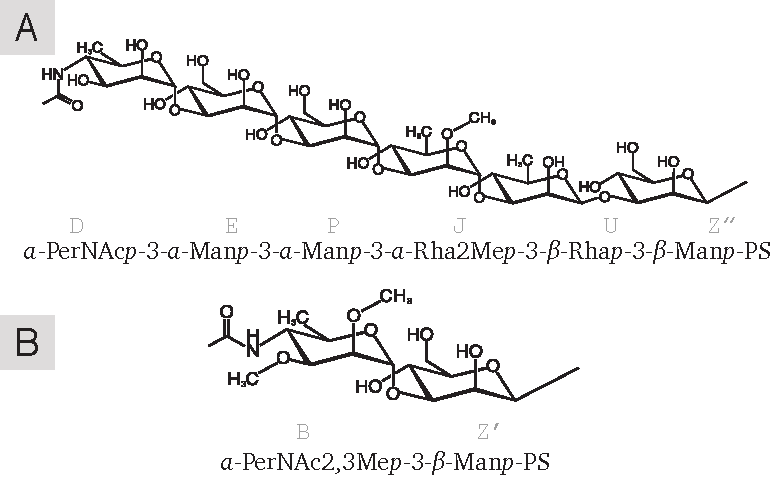
\includegraphics[]{lps_chapter/img/lpsends.pdf}
		 	\end{center}
		 	\caption[The structure of minor component, the end caps of the \ac{OPS}.]{The structure of minor component, the end caps of the \ac{OPS}. \textbf{A.} Fragment 1. \textbf{B.} Fragment 2.}
		 	\label{fig:lpsends}
		 \end{figure}

		 \begin{table}[htb]
			 \centering
			 \caption[\Ac{NMR} data for the minor components of the double oxidized non-deacylated \ac{PS}]{\ac{NMR} data for the minor components of the double oxidized non-deacylated \ac{PS} (50\cel). Methyl group signals: B2: 3.48/59.5; B3: 3.42/57.9; J2: 3.45/59.6 ppm (H/C)}
			 \label{tbl:lpsends}
			 \begin{tabular}{@{}rccccccc@{}}
				 \toprule
         &   & 1     & 2    & 3    & 4    & 5    & 6 \\ \midrule
				 \multirow{2}{*}{PerN2,3Me B}       & H & 5.25  & 3.96 & 3.71 & 3.81 & 3.91 & 1.17 \\
         & C & 100.2 & 76.2 & 78.2 & 53.2 & 69.5 & 18.0 \\
				 \multirow{2}{*}{$\alpha$-Rha2Me J} & H & 5.25  & 3.95 & 4.02 & 3.45 & 3.90 & 1.30 \\
         & C & 100.2 & 75.9 & 75.4 & 71.8 & 69.5 & 18.0 \\
				 \multirow{2}{*}{$\alpha$-PerN D}   & H & 5.14  & 4.27 & 4.20 & 3.95 & 3.97 & 1.23 \\
         & C & 100.1 & 67.4 & 75.2 & 52.2 & 69.4 & 18.0 \\
				 \multirow{2}{*}{$\alpha$-Man E}    & H & 5.13  & 4.17 & 3.99 & 3.75 & 3.84 & \\
         & C & 100.1 & 70.9 & 79.8 & 67.1 & 74.4 & \\
				 \multirow{2}{*}{$\alpha$-Man P}    & H & 5.05  & 4.14 & 4.00 & 3.85 & 3.96 & \\
         & C & 97.6  & 71.0 & 79.5 & 66.9 & 74.0 & \\
				 \multirow{2}{*}{$\beta$-Rha U}     & H & 4.78  & 4.16 & 3.69 & 3.48 & 3.44 & 1.32 \\
         & C & 100.9 & 71.8 & 82.0 & 72.4 & 73.1 & 18.0 \\
				 \multirow{2}{*}{$\beta$-Man Z"}    & H & 4.72  & 4.06 & 3.75 & 3.75 & 3.46 & 3.83; 3.96 \\
         & C & 98.2  & 71.9 & 86.0 & 67.0 & 77.4 & 62.1 \\
				 \multirow{2}{*}{$\beta$-Man Z'}    & H & 4.72  & 4.06 & 3.73 & 3.75 & 3.46 & 3.83; 3.96 \\
         & C & 98.2  & 71.9 & 82.3 & 67.0 & 77.4 & 62.1 \\ \bottomrule
			 \end{tabular}
		 \end{table} %
	% subsection minor_component_determination (end)

	\subsection{Rhamnan polysaccharide determination (\textsc{ps}2)} % (fold)
	\label{sub:rhamnan_polysaccharide_determination_ps2_}

  Periodate oxidation of the \ac{PS} produced an \ac{OS}1, which was analyzed by \ac{NMR} and its
  structure, as shown on \cref{fig:lpsrhamnan}, was determined using standard 2D \ac{NMR}
  methods. Signal assignment is shown in the \cref{tbl:lpsrhamnan}. It contained three
  rhamnopyranose units and 4-deoxy-1-deutero-erythritol, produced by the oxidation-reduction of
  4-substituted rhamnose. Formation of this oligosaccharide could be explained by oxidation of the
  side chain Rha F and 4-substituted Rha G in the \ac{PS}1 (letter labels for monosaccharides were
  given using anomeric signals in the whole \ac{PS} spectra starting from low-field). The unoxidized
  4-substituted residue T in the oligosaccharide originally carried side-chain Rha F at position
  2. Knowing the \ac{OS}1 structure the signals of a corresponding polymer (\ac{PS}2) were
  identified in the spectra of the whole \ac{PS}, and are given in the \cref{tbl:lpsrhamnan}.

		\begin{figure}[htb]
			\begin{center}
				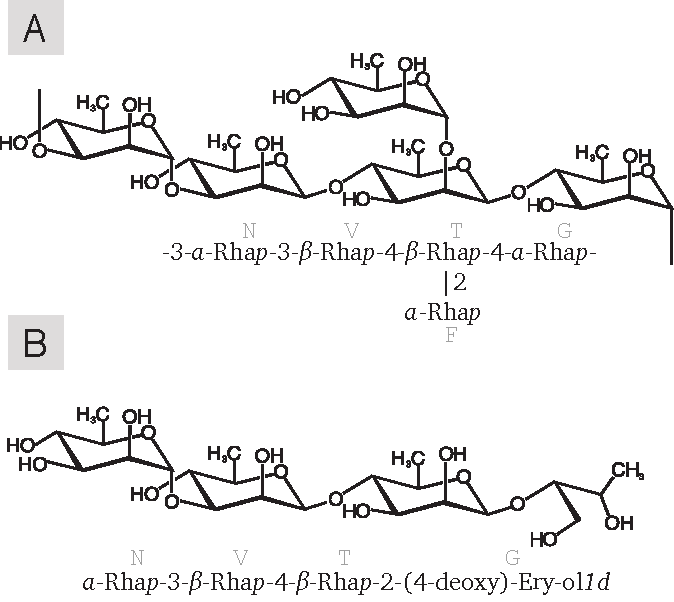
\includegraphics[]{lps_chapter/img/lpsrhamnan.pdf}
			\end{center}
			\caption[The structure of the \caulobacter rhamnan.]{The structure of the \caulobacter rhamnan. \textbf{A.} the intact rhamnan, \ac{PS}2. \textbf{B.} the oxidised rhamnan product, \ac{OS}1.}
			\label{fig:lpsrhamnan}
		\end{figure}

		\begin{table}[ht]
			\centering
			\caption[\Ac{NMR} data for \caulobacter  \ac{PS}2 and its \ce{NaIO4} oxidation product \ac{OS}1]{\ac{NMR} data for \caulobacter  \ac{PS}2 and its \ce{NaIO4} oxidation product \ac{OS}1 (40\cel).}
			\label{tbl:lpsrhamnan}
			\begin{tabular}{@{}rccccccc@{}}
				\toprule
				                                     &   & 1          & 2    & 3    & 4    & 5    & 6 \\ \midrule
				\multirow{2}{*}{$\alpha$-Rha N, OS1} & H & 5.04       & 4.07 & 3.85 & 3.47 & 3.85 & 1.30 \\
				                                     & C & 103.1      & 71.1 & 71.1 & 72.9 & 69.9 & 17.6 \\
				\multirow{2}{*}{$\alpha$-Rha N, PS}  & H & 5.02       & 4.02 & 3.79 & 3.45 & 3.72 & 1.28 \\
				                                     & C & 103.0      & 71.5 & 78.8 & 73.3 & 70.4 & 17.5 \\
				\multirow{2}{*}{$\beta$-Rha T, OS1}  & H & 4.78       & 4.13 & 3.71 & 3.54 & 3.53 & 1.33 \\
				                                     & C & 100.7      & 71.1 & 72.3 & 83.4 & 71.7 & 17.5 \\
				\multirow{2}{*}{$\beta$-Rha T, PS}   & H & 4.79       & 4.22 & 3.82 & 3.62 & 3.61 & 1.36 \\
				                                     & C & 101.7      & 76.7 & 73.5 & 83.4 & 73.2 & 17.5 \\
				\multirow{2}{*}{$\beta$-Rha V, OS1}  & H & 4.75       & 4.12 & 3.67 & 3.49 & 3.49 & 1.34 \\
				                                     & C & 101.1      & 71.4 & 81.3 & 71.9 & 72.9 & 17.5 \\
				\multirow{2}{*}{$\beta$-Rha V, PS}   & H & 4.77       & 4.13 & 3.66 & 3.66 & 3.50 & 1.35 \\
				                                     & C & 101.4      & 71.2 & 81.7 & 67.2 & 73.3 & 17.5 \\
				\multirow{2}{*}{X (ox. G), OS1}      & H & 3.69; 3.71 & 3.75 & 3.99 & 1.20 &      & \\
				                                     & C & 61.8       & 84.8 & 67.7 & 18.0 &      & \\
				\multirow{2}{*}{$\alpha$-Rha G, PS}  & H & 5.10       & 4.13 & 3.94 & 3.58 & 3.90 & 1.35 \\
				                                     & C & 103.1      & 71.5 & 70.3 & 84.5 &      & 17.5 \\
				\multirow{2}{*}{$\alpha$-Rha F, PS}  & H & 5.11       & 4.09 & 3.87 & 3.45 & 4.07 & 1.27 \\
				                                     & C & 102.4      & 72.1 & 71.3 & 73.3 &      & 17.5 \\ \bottomrule
			\end{tabular} %% LPS Rhamnan
		\end{table}
	% subsection rhamnan_polysaccharide_determination_ps2_ (end)

	\subsection{Core oligosaccharide determination} % (fold)
	\label{sub:core_oligosaccharide_determination}

  The core oligosaccharide of the \caulobacter{} \ac{LPS} isolated after \ce{AcOH} hydrolysis
  contained one non-degraded Kdo, two LD-Hep, one DD-Hep, mannose, galactose, and glucuronic acid in
  pyranose form. 2D \ac{NMR} analysis led to the structure shown on \cref{fig:lpscore} (\ac{NMR}
  assignments are in \cref{tbl:lpstable4}, the \ac{HSQC} spectrum is in \cref{fig:lpscorenmr}). The
  sequence followed from the observed \ac{NOE}: E1:C5,C7,F5; F1:E2; G1:F3; H1:C7,E2; K1:C4;
  L1:K4. Correlation E1:C7 is always observed in the $\alpha$-Hep-5-Kdo fragment. E1:F5 was due to
  the $\alpha$-Man-2-Hep linkage. H1E2 indicates spatial proximity of the residues E and H, linked
  to the same Kdo C. All expected transglycoside correlations were observed in \ac{HMBC} spectrum,
  together with intra-ring correlations H-1:C-3 and H-1:C-5 for all $\alpha$-pyranoses. Methylation
  analysis revealed terminal DD-Hep, terminal and 2-substituted LD-Hep, 3-substituted Man and
  terminal Gal. The structure agreed with mass spectral data, \ac{ESI} \ac{MS} in negative ion mode,
  [M-H]\textsuperscript{-} = 1314.9, [M-2H]/2\textsuperscript{-} = 656.7, calculated exact mass Hex
  x 2 + Hep x 3 + HexA x 1 + Kdo x 1 = 1314.4 Da.

		\begin{figure}[htb]
			\begin{center}
				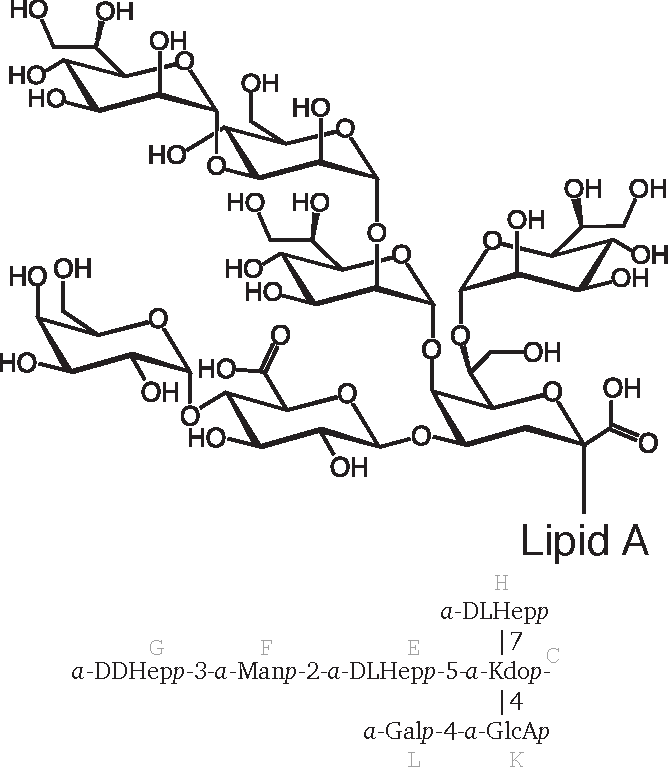
\includegraphics[]{lps_chapter/img/lpscore.pdf}
			\end{center}
			\caption{The structure of the \caulobacter core \ac{OS}.}
			\label{fig:lpscore}
		\end{figure}

		\begin{table}[htb]
			\centering
			\caption[\Ac{NMR} data for the core oligosaccharide]{\ac{NMR} data for the core oligosaccharide (25\cel).}
			\label{tbl:lpstable4}
			\begin{tabular}{@{}rccccccccc@{}}
        \toprule
        &   & 1     & 2    & 3          & 4    & 5    & 6          & 7          & 8 \\ \midrule
        \multirow{2}{*}{Kdo C}   & H &       &      & 2.05; 2.35 & 4.23 & 4.28 & 4.09       & 3.91       & 3.81; 3.93 \\
        & C &       & 98.2 & 34.7       & 74.9 & 74.2 & 71.0       & 79.2       & 61.5 \\
        \multirow{2}{*}{DLHep E} & H & 5.24  & 3.85 & 4.12       & 3.89 & 3.88 & 4.04       & 3.73; 3.73 & \\
        & C & 101.1 & 80.2 & 71.1       & 67.3 & 74.1 & 70.0       & 63.9       & \\
        \multirow{2}{*}{Man F}   & H & 5.03  & 4.30 & 4.00       & 3.79 & 3.80 & 3.80; 3.91 &            & \\
        & C & 103.7 & 70.6 & 78.1       & 67.5 & 74.5 & 62.0       &            & \\
        \multirow{2}{*}{DDHep G} & H & 5.15  & 4.05 & 3.86       & 3.77 & 3.84 & 4.06       & 3.76; 3.84 & \\
        & C & 103.1 & 71.0 & 71.8       & 68.7 & 74.5 & 72.9       & 62.9       & \\
        \multirow{2}{*}{DLHep H} & H & 5.07  & 4.14 & 3.89       & 3.89 & 3.80 & 4.10       & 3.79; 3.81 & \\
        & C & 102.7 & 73.7 & 71.8       & 67.3 & 73.2 & 70.2       & 64.9       & \\
        \multirow{2}{*}{GlcA K}  & H & 5.22  & 3.66 & 4.00       & 3.99 & 4.15 &            &            & \\
        & C & 98.8  & 72.4 & 74.9       & 73.6 &      &            &            & \\
        \multirow{2}{*}{Gal L}   & H & 5.49  & 3.80 & 3.85       & 3.99 & 3.94 & 3.69; 3.69 &            & \\
        & C & 99.9  & 69.7 & 70.3       & 70.0 & 71.8 & 61.6       &            & \\ \bottomrule
			\end{tabular}%LPS table 4
		\end{table}

		\begin{figure}[htb]
			\begin{center}
				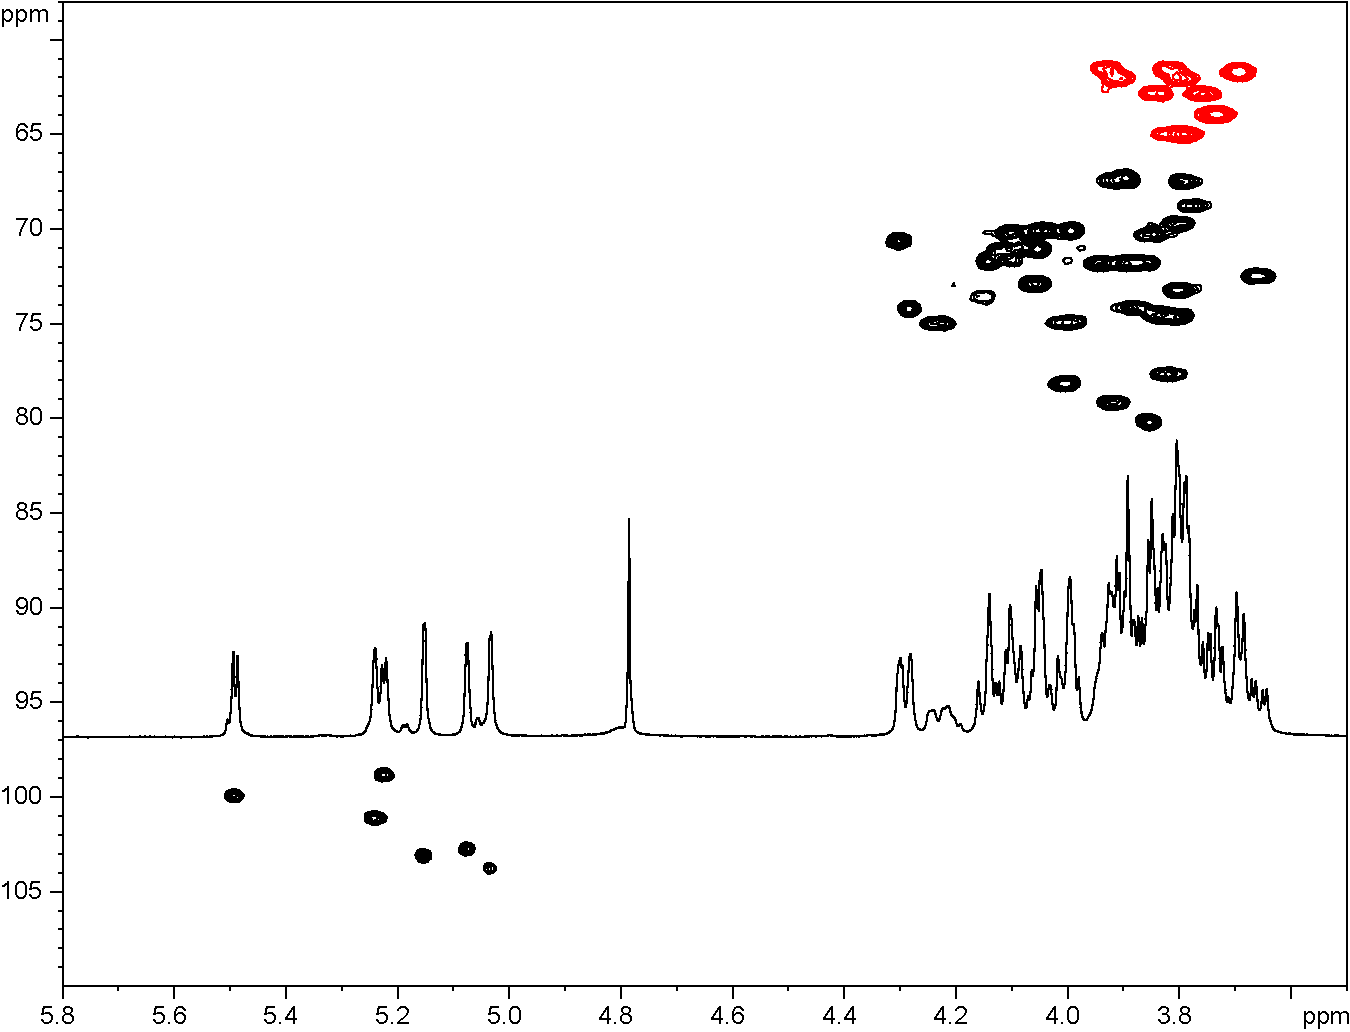
\includegraphics[width=\textwidth]{lps_chapter/img/lpsfig4.pdf}
			\end{center}
			\caption{Fragment of \textsuperscript{1}H-\textsuperscript{13}C \ac{HSQC} spectrum of the core.}
			\label{fig:lpscorenmr}	
		\end{figure}
    % subsection core_oligosaccharide_determination (end)
    \subsection{Cellular response to \textit{C. crescentus} LPS}\label{sec:cell-resp-text}

   \begin{figure}[htb]
  	\begin{center}
   		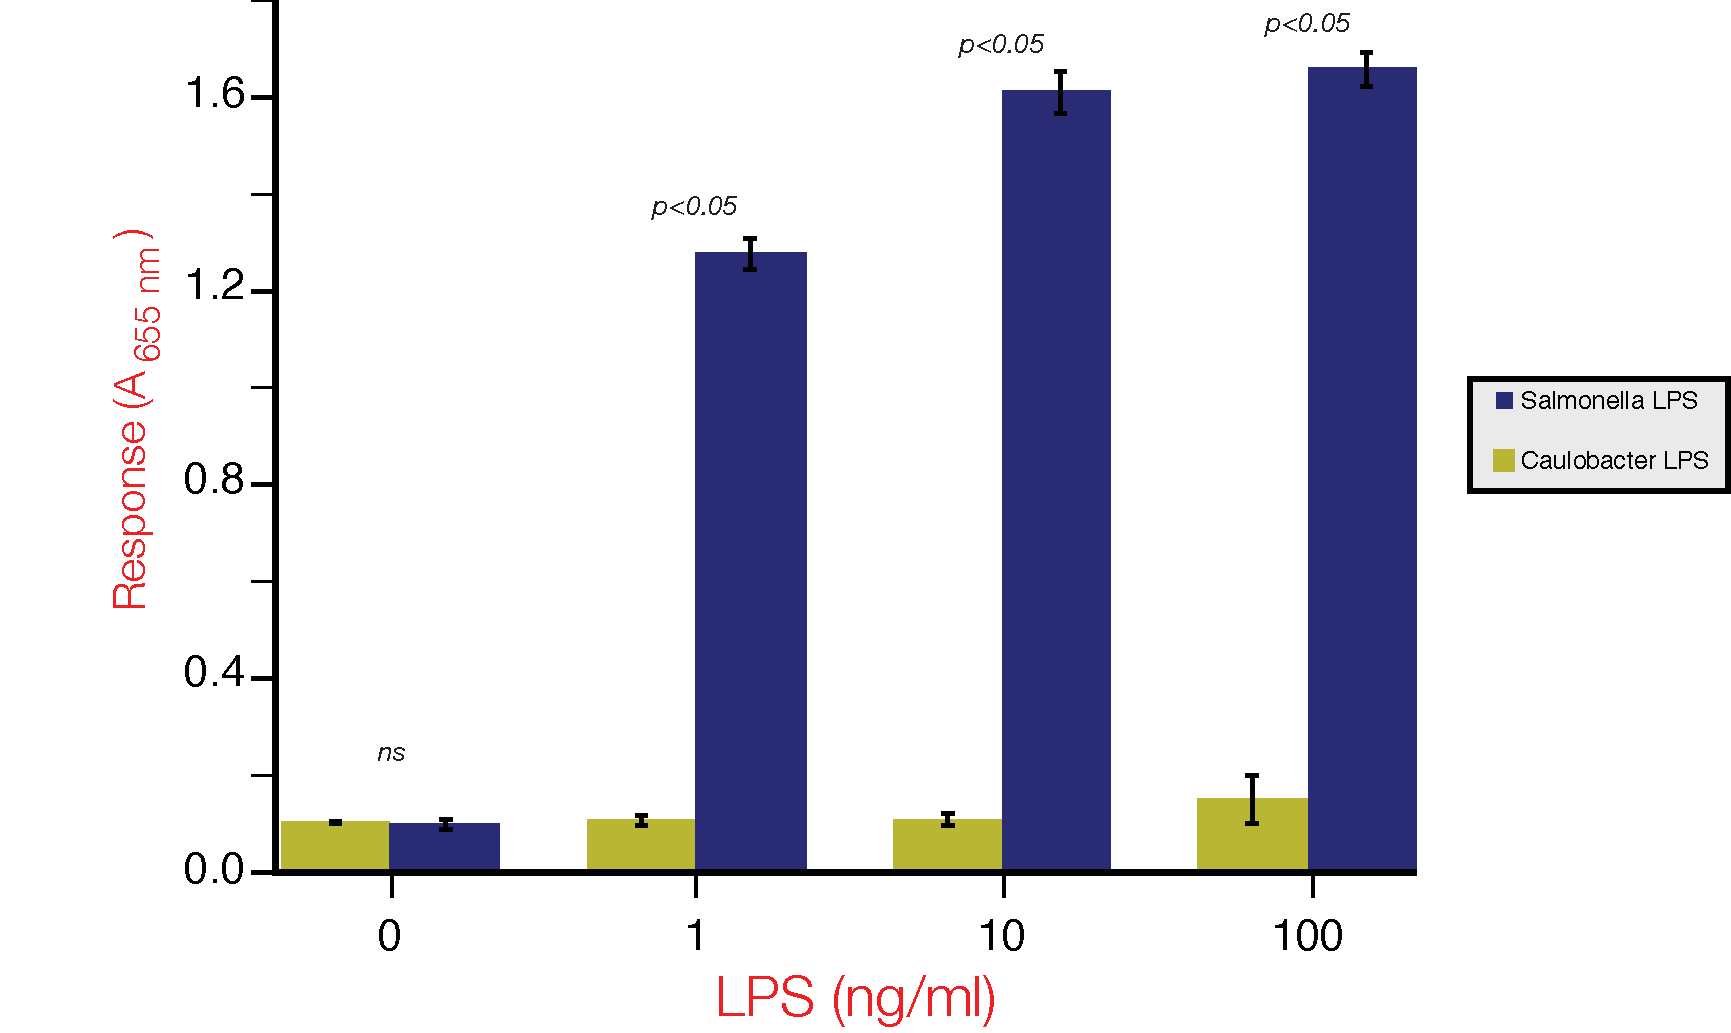
\includegraphics[width=\textwidth]{lps_chapter/img/NFkBAssay.pdf}
   	\end{center}
   	\caption[NF$\kappa$B Assay for cellular activation by LPS]{
	   	\textbf{TITLE} TEXT % Add adescription!
   	}
   	\label{fig:nfkbassay}
\end{figure}    
% section results (end)


\section{Methods} % (fold)
\label{sec:lps_methods}

	\subsection{Bacterial strain construction and growth conditions} % (fold)
	\label{sub:bacterial_strain_construction_and_growth_conditions}

  The strain used for the preparation of \ac{LPS} was JS1025, a derivative of \caulobacter CB15
  NA1000. The salient features are that it has an engineered amber mutation in \textit{rsaA} leading
  to the loss of the \ac{S-layer} and the gene CCNA\_00471 has been inactivated by a partial
  deletion. CCNA\_00471 encodes a putative GDP-L-fucose synthase\upcite[.]{na1000genome} The
  knockout (\del 471) confers a deficiency in an \ac{EPS} that was previously found to contain
  L-fucose\upcite[.]{ravenscrofteps} CCNA\_00471 was disrupted in the same manner as previously in
  JS4038\upcite[,]{hivmicrobicide2} except the starting strain used here was
  JS1023\upcite[.]{slayercryo}
		
  Cells were grown to mid-to-late log phase (\od = 0.9) in M16HIGG defined medium at 30\cel in 2.8
  \si{\litre} Fernbach flasks containing 1250 \millilitre of medium, shaking at 100 rpm. M16HIGG is
  a modification of M6HIGG medium\upcite[,]{smitpilin81} containing 0.31\% glucose, 0.09\%
  glutamate, 1.25 \si{\milli\meter} sodium phosphate, 3.1 \si{\milli\meter} imidazole, 0.05\%
  ammonium chloride, and 0.5\% modified Hutner's Mineral Base\upcite[.]{hutners}
	% subsection bacterial_strain_construction_and_growth_conditions (end)

	\subsection{\textsc{lps} isolation} % (fold)
	\label{sub:LPS_isolation}
  \ac{LPS} was isolated from the cells via disrupting the outer membrane by chelation.  The the
  negative charges in Gram negative bacterial \ac{LPS} are stabilised and bridged by available
  divalent cations (\ie{} \ce{Ca^2+} and \ce{Mg^2+}). Lieve first noted in 1965\upcite{leive65} that
  one can strip the counter ions from the outer membrane to disrupt it and cause it to shed into the
  medium. We chose a chelation strategy because we found it easy to scale up, it didn't require
  noxious organic solvents, and because our lab's first attempt to isolate and analyse \caulobacter\
  \ac{LPS}\upcite{ravenscroftlps} using the Darveau extraction method\upcite{darveauprocedure} only
  resulted in the isolation of core+lipidA (rough \ac{LPS}).

  The protocol we used was a modification of the procedure reported by Walker
  \etal\!\upcite{walker94} Cells were centrifuged at 12 400 x g for 10 min. The pellets were
  suspended with distilled water and recentrifuged. These pellets were resuspended in 1/10 original
  culture volume in \ac{PBS}\upcite{maniatis} amended with 35 \si{\milli\meter} \ac{EDTA}, agitated
  at room temperature for 10 min and then centrifuged at 15 300 x g for 15 min. The supernatant was
  retrieved and re-centrifuged, as before, to ensure clarity and then dialysed against 5
  \si{\milli\meter} \ce{MgCl2}. DNase and RNase were added to final concentrations of 10
  \si{\micro\gram\per\milli\litre} and 100 \si{\micro\gram\per\milli\litre}\!, respectively, and
  incubated at 37\cel for 2 h. Proteinase K was added to a final concentration of 0.3 \mgperml and
  the preparation was incubated at 50\cel overnight. The sample was then ultracentrifuged at 184 000
  x g for 3 h. Glassy pellets formed which were suspended in distilled water to 1/100 original
  culture volume. A Bligh-Dyer extraction was performed to reduce contaminating
  lipids\upcite[.]{blighdyer}
	% subsection \ac{LPS}_isolation (end)

	\subsection{Bligh Dyer Extraction} % (fold)
	\label{sub:bligh_dyer_extraction}
  A Bligh Dyer extraction was performed on all \ac{LPS} preparations to reduce the presence of
  contaminating lipids. The extraction was performed as first published\upcite[.]{blighdyer} In
  short, to one volume of aqueous \ac{LPS} sample, 3.75 volumes of chloroform/methanol (1:2 v/v) was
  added and the sample was vortexed for 30 seconds. 1.25 volumes of chloroform was added and the
  sample was vortexed again for 30 seconds. 1.25 volumes of water were added and the sample was
  vortexed a final time for 30 seconds. This mixture was then centrifuged at 15 300 x g for 10
  min. After centrifugation, the mixture separated in to two phases, a lower organic phase and an
  upper aqueous phase. The \ac{LPS} partitions into the aqueous phase, while other lipids partition
  into the organic phase. The aqueous phase was retrieved and kept.
	% subsection bligh_dyer_extraction (end)

	\subsection{Silver stain and gel electrophoresis} % (fold)
	\label{sub:gel_electrophoresis}

  Discontinuous \ac{SDS-PAGE} was performed with a 13\% separating gel\upcite[.]{laemmli} Detection
  of \ac{LPS} was done by periodate oxidation and silver staining as described by Zhu
  \etal\!\upcite{improvedsilverstain} The silver stain protocol is a newer technique that uses
  vitamin C (ascorbic acid) in place of formaldehyde in traditional \ac{LPS}
  stains\upcite[.]{tsai1982sensitive} Table \ref{tbl:silver} give the details of the silver stain
  procedure.

		% Please add the following required packages to your document preamble:
		% \usepackage{booktabs}
		\begin{table}[ht]  % Silver stain table
			\centering
			\caption{\Ac{LPS} silver stain procedure}
			\label{tbl:silver}
			\begin{tabular}{@{}rcl@{}}
				\toprule
				\textbf{Step} & \textbf{Solution}                                                           & \textbf{Time} \\ \midrule
				Oxidation     & 30\% EtOH, 10\% HOAc, 0.7\% periodic acid                                   & 10 	min     \\
				Rinse         & d\ce{H2O}                                                                   & 5 min x2   \\
				Silver        & 0.2\% \ce{AgNO3}                                                            & 5 min      \\
				Rinse         & d\ce{H2O}                                                                   & 20 sec x2  \\
				Develop       & 3\% \ce{NaCO3}, 0.04\% \ce{Na2S2O3}, 0.02\% ascorbic acid, 0.05\% \ce{NaOH} & 8 min      \\
				Stop          & 10\% HOAc                                                                   & 1 min \\ \bottomrule
			\end{tabular}
		\end{table}
	% subsection gel_electrophoresis (end)
    \subsection{Preparation of RsaA \del 277--784 probe} \label{sec:preparation-rsaa-del}
    
    The plasmid, p4BRsaA\del 277--784, was extant in our laboratory from the work of Wade Bingle. In short, various versions of rsaA were engineered to have \textit{Bam}HI sites at locations throughout the gene\upcite[.]{bingle1997linker} The \textit{Bam}HI--\textit{Hin}DIII fragment from a version of rsaA with a \textit{Bam}HI site at the 831 bp from the start codon was replaced with a \textit{Bam}HI--\textit{Hin}DIII fragment from a version of rsaA with a \textit{Bam}HI site at the 2352 bp position. In effect this made a rsaA gene missing 1521 bp from the center, corresponding to amino acids 277--784 within the resulting protein. This `internally truncated' gene was then moved into the context of our expression vector `p4B'\upcite[]{lau2010analysis} as a \textit{Eco}RI--\textit{Hin}DIII fragment.
    
    \subsection{Periodic acid-Schiff Stain} % (fold)
    \label{sub:schiff_stain}
		
    Periodic   acid-Schiff   stain   was   performed   on  \ac{LPS}   samples   that   were   run   on
    \ac{SDS-PAGE}. Schiff stain is analogous to silver  stain in that it identifies carbohydrates that
    are first oxidised with periodic acid.

    The staining procedure starts by soaking the gel on a slow shaker in 0.7\% periodic acid in
    distilled water for 15 min. The gel is then rinsed in distilled water and placed in Schiff reagent
    and shaken slowly for 15 min. The gel is then washed in distilled water for 5 min, at which time
    pink bands should appear that are correspond to polysaccharides/\ac{LPS} in the gel.

    The protocol to prepare Schiff's reagent started by dissolving 5 \si{\gram} of basic fuchsin in
    900 \millilitre of boiling distilled water. Once dissolved the fuchsin solution was removed from
    heat and allowed to cool for a few minutes, then 100 \millilitre of 1 \si{\molar}\ \ce{HCl} was
    slowly added. After the solution was allowed to cool to room temperature, 10 \si{\gram} of
    \ce{K2S2O5} was added. This solution was thoughly mixed, then incubated in the fume hood
    overnight. The next day, a few spoonfuls of activated charcoal were added to the Schiff reagent to
    decolourize the solution. The solution was stired and then filtered through Watman paper \# 1. The
    now clear Schiff stain solution was ready to use. It had a sulfurous smell and would stain nearly
    any surface it was spilled on a vibrant pink colour. A test for Schiff reagent activity would be
    to add a few drops of Schiff reagent to 5 \millilitre of formaldehyde in a test tube. The mixture
    should instantly turn a bright pink colour, indicating activity.
    % subsection schiff_stain (end)

      \subsection{\textsc{nmr} spectroscopy} % (fold)
      \label{sub:nmr_spectroscopy}

      \ac{NMR} experiments were carried out on a Varian INOVA 600 \si{\mega\hertz}
      (\textsuperscript{1}H) spectrometer with 5 \si{\milli\meter} gradient probe at 25--50\cel with
      acetone internal reference (2.225 ppm for \textsuperscript{1}H and 31.45 ppm for
      \textsuperscript{13}C), using standard pulse sequences \ac{gCOSY}, \ac{TOCSY}(mixing time 120
      \si{\milli\second}), \ac{ROESY} (mixing time 300 \si{\milli\second}), \ac{gHSQC}, and
      \ac{gHMBC}(100 \si{\milli\second} long range transfer delay), \ac{HMQC} for
      \textsuperscript{1}H-\textsuperscript{31}P correlation, J$_{HX}$ set to 10
      \si{\hertz}. Acquisition time was kept at 0.8--1 sec for H-H correlations and 0.25 sec for
      \ac{HSQC}. 256 increments were acquired for t$_1$ in all 2D spectra, except 512 for \ac{gCOSY}.
      % subsection nmr_spectroscopy (end)

      \subsection{\textsc{lps} Chromatography} % (fold)
      \label{sub:chromatography}

      Gel chromatography was performed on a Sephadex G-15 column (1.5 x 60 \si{\centi\meter}) or a
      Bio-gel P6 column (2.5 x 60 \si{\centi\meter}) in pyridine-acetic acid buffer (4 \millilitre:10
      \millilitre:1 \si{\litre} water), and monitored by refractive index detector (Gilson). Anion
      exchange chromatography was done on an Hitrap Q column (2x5 \millilitre size, Amersham), with
      \ac{UV} monitoring at 220 nm in a linear gradient of \ce{NaCl} (0--1 M, 1 h) at the 3
      \si{\milli\litre\per\minute}. Fractions of 1 min were collected and additionally tested for
      carbohydrates, by spotting on an \ce{SiO2} \ac{TLC} plate, dipping them in 5\% \ce{H2SO4} in
      \ce{EtOH} and heating with a heat-gun. All fractions of interest were dried in a Savant drying
      centrifuge and \textsuperscript{1}H spectra were recorded for each fraction without desalting. For
      2D \ac{NMR}, desalting was performed on a Sephadex G15 column.
      % subsection chromatography (end)x`'

      \subsection{Monosaccharide analysis} % (fold)
      \label{sub:monosaccharide_analysis}

      Samples with added inositol standard were hydrolysed with 3 M \ac{TFA} at 120\cel. Monosaccharides
      were converted to alditol acetates by conventional methods and identified by \ac{GC-MS} on a
      Varian Saturn 2000 instrument on a DB17 capillary column (30 m x 0.25 \si{\milli\meter} ID x 0.25
      \si{\micro\meter} film) with helium carrier gas, using a temperature gradient 170\cel (3
      min)--250\cel at 5\si{\degreeCelsius\per\minute}.
      % subsection monosaccharide_analysis (end)

      \subsection{Determination of absolute configurations of monosaccharides} % (fold)
      \label{sub:determination_of_absolute_configurations_of_monosaccharides}

      To the polysaccharide sample (0.2 \milligram) (R)-2-\ce{BuOH} (0.2 \millilitre) and acetyl
      chloride (0.02 \millilitre) were added at room temperature, heated at 90\cel for 2 h, dried by air
      stream, acetylated, analysed by \ac{GC-MS} as described above. Standards were prepared from
      monosaccharides of known configuration with (R)- and (S)-2-\ce{BuOH}.
      % subsection determination_of_absolute_configurations_of_monosaccharides (end)

      \subsection{Methylation analysis} % (fold)
      \label{sub:methylation_analysis}

      For the methylation analysis core sample (2 \milligram) was dephosphorylated with 50 \microlitre
      of 48\% \ce{HF} for 20 h at +10\cel, diluted with 2 \millilitre of ethanol, precipitate collected
      by centrifugation, washed with 2 \millilitre of ethanol, dried.

      Methylation was performed by Ciucanu-Kerek procedure\upcite[.]{ciucanufrancisc} 0.5 \milligram of
      the sample was dissolved in 0.5 \millilitre of dry DMSO with heating at 100\cel for 5-10 min until
      complete dissolution. Powdered \ce{NaOH} (about 50 \milligram) was added and the mixture was
      stirred for 30 min. 0.2 \millilitre of \ce{MeI} was added and the mixture was stirred for a
      subsequent 30 min. The sample was then flushed with air to remove the MeI and diluted to 10
      \millilitre with water. The sample was passed through a C18 Seppak cartridge, washed with 10
      \millilitre of water, and then the methylated compound was eluted with 5 \millilitre of
      methanol. The methylated product was hydrolysed with 3 M \ac{TFA} (120\cel, 3h), dried, reduced
      with \ce{NaBD4}, and the reagent destroyed with 0.5 \millilitre of 4 M \ce{HCl}. The solution was
      dried under a stream of air and dried twice more with the addition of \ce{MeOH} (1
      \millilitre). The sample was acetylated with 0.4 \millilitre{} \ce{Ac2O} and 0.4 \millilitre
      pyridine for 30 min at 100\cel. It was then dried and analysed by \ac{GC-MS}.
      % subsection methylation_analysis (end)

      \subsection{Periodate oxidation} % (fold)
      \label{sub:periodate_oxidation}

      \ac{PS} (10 \milligram) was dissolved in water (2 \millilitre). \ce{NaIO4} (20 \milligram) was
      added and the solution was incubated at room temperature for 24 h. Ethylene glycol (0.2
      \millilitre) and an excess \ce{NaBD4} were added. The solution was then kept for 1 h before being
      treated with 0.2 \millilitre of \ce{AcOH} and desalted on a Sephadex G-15 column. The product was
      hydrolysed with 2\% \ce{AcOH}, 2 h at 100\cel, and separated on a Sephadex G-50 column to give
      \ac{OS}1.
      % subsection periodate_oxidation (end)
      % section methods (end)

      \section{Discussion} % (fold)
      \label{sec:lps_discussion}

      The \ac{LPS} of \caulobacter has an unusually complicated structure with two different
      polysaccharides, irregular substituents, and unfavourable \ac{NMR} spectra. Presented data show
      structures of the core part, two polymers, and putative terminal structures. The polysaccharides
      could not be separated by size exclusion or anion-exchange chromatography and are probably linked
      together through the same core. The core of the \caulobacter{} \ac{LPS} has been studied previously
      and an initial assessment of its composition was made\upcite[,]{ravenscroftlps} but the complete
      structure had not been determined. The structure of the \ac{OPS} has not been studied before. In our
      view the polysaccharide structure of the \caulobacter{} \ac{LPS} represents one of the most
      complicated bacterial \ac{LPS} polysaccharide structures identified so far.

      The Kdo present in the \ac{LPS} core structure (see \cref{fig:lpscore}) has the typical
      substitutions at O-4 and O-5 of a manno-configured sugar and a negatively charged sugar,
      respectively\upcite[.]{brade99} It also has a rarely observed third substitution at O-7 with a
      heptose moiety. The Kdo O-7 position is known to be occupied by a galactose moiety in the core of
      \textit{Rhizobium leguminosarum} bv. Viciae VF39\upcite[,]{rhizobiumlps} and the secondary Kdo in
      the core oligosaccharide from \textit{Acinetobacter baumannii} ATCC 19606 has an O-7 substituted
      with a glucosamine\upcite[.]{acinetobacterlps}

      In the traditional model \ac{LPS} occupies the outer leaflet of the outer membrane of a
      Gram-negative bacterium, and so (excepting the presence of cell associated \ac{EPS}) is the
      outermost layer of the cell. For \caulobacter, however, \ac{LPS} is the penultimate barrier below
      the protein \ac{S-layer}. The \caulobacter{} \ac{OPS} serves as the anchor for the S-layer and is
      likely not accessible to the environment\upcite[.]{walker94} The carbohydrates found in the \ac{OPS}
      are particularly hydrophobic, marked by the abundance of deoxy-sugars, acetyl groups, and methyl
      groups. This hydrophobicity is possibly a result of particular sugars needed for \ac{S-layer}
      anchoring, as these carbohydrate structures likely evolved as the cognate ligands for the
      \ac{S-layer} protein, RsaA. The distance between the \ac{S-layer} and the outer membrane is about
      17--19 nm\upcite[.]{dipm} It is possible the hydrophobicity aids in packing the polysaccharides
      between the S-layer and the \ac{LPS}. Further determination of RsaA's structure should help
      illuminate the interaction between the S-layer and \ac{OPS}.

      Knowledge of the structure of \caulobacter{} \ac{OPS} and \ac{LPS} will facilitate the determination
      and characterization of their biosynthetic enzymes and mutant variants. Already, the enzymes
      LpxI\upcite{lpxi} and GDP-L-perosamine acetylase\upcite{perosmineacetyltransferase} from
      \caulobacter have been characterized. One uncharacterised enzyme, WbqL, is necessary for proper
      \ac{OPS} synthesis and disruption of wbqL leads to the accumulation of truncated and S-layer
      anchoring deficient \ac{OPS} in the inner membrane and inhibits Crescentin-mediated cell
      curvature\upcite[.]{lpsinterferecrescentin} Many genes, such as wbqL, have been identified as
      essential for \ac{OPS} synthesis\upcite{awramgenes} but have not yet been characterized. Other
      genes, that must be essential for \ac{OPS} synthesis, have yet to be identified or characterized,
      such as the O-antigen polymerase and ligase.

      % --Should I increase the text about lpxI?--%

      The subunit-based repeating nature of \caulobacter{} \ac{OPS} suggests that a Wzy-dependent pathway
      synthesizes the polymer\upcite[.]{lpsreview02} The previous study that aimed to identify genes
      essential for \ac{OPS} did not identify many of the canonical genes in the Wzy-dependant
      pathway\upcite[,]{awramgenes} such as the O-unit transporter, Wzx, O-antigen polymerase, Wzy; the
      chain-length determinate protein, Wzz; and the O-antigen ligase, WaaL. Genes that have been
      annotated as putative O-antigen synthesis genes do appear in the sequenced genomes for \caulobacter
      CB15, but they have not been experimentally confirmed.

      An additional aspect to this \ac{LPS} it the fact that its O-antigen is of homogeneous length. While
      other \ac{LPS}s vary in size due to the number of O-antigen repeat groups, appearing as a laddering
      of bands by \ac{SDS-PAGE}, the \ac{LPS} from \caulobacter appears as a single
      band\upcite[.]{walker94} Initial \ac{MALDI-TOF} analysis of the entire \ac{LPS} indicates a size of
      about 10.8 kDa (see \cref{fig:lpsmalditof} on \cpageref{fig:lpsmalditof}).  After accounting for the
      solved structures for the lipid A and core regions, this suggests the \ac{LPS} contains
      approximately 5 repeats of the proposed heptameric O-antigen structure.  There is not currently a
      known mechanism for the regulation and synthesis of a strictly homogeneous length O-antigen. It is
      possible that this \ac{OPS} is synthesized via the \ac{ABC}-transporter-dependent
      pathway\upcite{lpsreview02} or another heretofore undiscovered mechanism. In any event it would seem
      that the transfer of a polysaccharide of this considerable size to the outer leaflet of the outer
      membrane is a remarkable feat for the bacterium.

	%% The following is a directive for TeXShop to indicate the main file
%!TEX root = ../MJThesis.tex
\acresetall
\chapter{OmpW of \textit{Caulobacter crescentus} functions as an outer membrane channel}
\label{ch:porin}
\begin{epigraph}
  \emph{``We must never let ourselves fall in thinking `ignorabimus' (`We shall never know'), but must have every confidence that the day will dawn when even those processes of life which are still a puzzle today will cease to be inaccessible to us natural scientists.''} ---~Eduard~Buchner,~1907~Nobel~lecture 
\end{epigraph}
\section{Introduction} % (fold)
\label{sec:porin_introduction} 
\lettrine[lines=2]{G}{ram-negative} bacterial cell-envelopes consist of different layers. The inner, or cytoplasmic, membrane contains the respiration chain, proteins for the transport of nutrients, and proteins involved in the synthesis of phospholipids, peptidoglycan, and lipopolysaccharides\upcite[.]{beveridge1981ultrastructure, nikaido1985molecular} The periplasmic space between the membranes is an aqueous compartment isoosmolar to the cytoplasm\upcite[.]{benz1994uptake} It contains the peptidoglycan and a large number of different proteins. The outer membrane is composed of protein, lipid and \ac{LPS}\upcite[.]{beveridge1981ultrastructure} It typically contains only a few major proteins. Normally at least one of the constitutive outer membrane proteins is a porin, a general diffusion pore with a defined exclusion limit for hydrophilic solutes\upcite[.]{nikaido2003molecular} In addition to constitutive porins, an outer membrane may contain porins that are induced under special growth conditions\upcite[.]{benz2001porins} They often form solute-specific channels and contain binding sites for neutral substrates such as carbohydrates\upcite[,]{benz1986pore, ferenci1980lambda} or nucleosides\upcite[,]{benz1986pore} and phosphate\upcite[.]{benzhancock1987mechanism, hancock1982outer} Many of the specific porins are part of uptake and degradation systems, such as the maltose uptake system of \ac{ecoli}\upcite[.]{schwartz1987maltose} 

    \ac{caulobacter}, a member of the alphaproteobacteria group, is a Gram-negative bacterium found in oligotrophic aquatic environments\upcite[.]{curtis2010getting} \ac{caulobacter} has well been studied as a model of cell cycle and bacterial differentiation\upcite[.]{mcadams2003bacterial} Its genome sequence has been known for more than 10 years\upcite[.]{caulobactergenomeseq} \ac{caulobacter} is an unusual Gram-negative bacterium in that genes coding for typical general diffusion porins of the OmpF/C type of enteric Gram-negative bacteria have not been identified in its genome\upcite[.]{lohmiller2008tonb, neugebauer2005exbbd, caulobactergenomeseq} Similarly, genes coding for specific porins such as Tsx or LamB are also absent. Instead, the genome of \ac{caulobacter} contains a large number of genes that code for TonB-dependent receptors\upcite[.]{lohmiller2008tonb, neugebauer2005exbbd} More than 60 of these receptors have been identified\upcite[,]{lohmiller2008tonb} which probably means that most of the nutrients from dilute environments are taken up actively by these systems. Examples for this are the uptake of maltose and \ac{glcnac} into the cells\upcite[.]{eisenbeis2008naga, lohmiller2008tonb}

    In this study we investigated whether the outer membrane of \ac{caulobacter} also contained a porin-like channel. The results suggested that despite the assumption that the \ac{caulobacter} outer membrane does not contain porins; a porin-like channel could be detected in artificial membranes with a single-channel conductance of about 125 \si{\pico\sievert} in 1 \si{\molar} \ce{KCl}. The protein responsible for channel formation was identified to be a member of the large OmpW family of outer membrane proteins. OmpW analogue proteins are found in many Gram-negative bacteria. Two members of this family, OmpW of \ac{ecoli} and OprG of \ac{pseudomonas} have been crystallized and their 3D-structures are known at high resolution (3.5 and 2.7 and 2.4 \AA, respectively)\upcite[.]{albrecht2006expression, hong2006outer, touw2010crystal} Here we show that OmpW of \ac{caulobacter} functions as a channel for cations, which is in sharp contrast to OprG of \ac{pseudomonas} and OmpW of \ecoli, which are believed to be plugged completely or involved in the transport of small, yet unknown hydrophobic molecules across the cell wall of these bacteria\upcite[.]{albrecht2006expression, hong2006outer, touw2010crystal} The 3D-structure of OmpW of \ac{caulobacter} was modeled on the basis of the known structures of OmpW of \ac{ecoli} and OprG of \ac{pseudomonas}\upcite[.]{hong2006outer, touw2010crystal} The results indicated that OmpW of \ac{caulobacter} could have a larger diameter and more hydrophilic interior than the two crystallized members of the OmpW family.

\section{Methods and Materials}
\label{sec:porin_methods}
\subsection{Growth and maintenance of microorganisms} 
\label{sub:porin_growth}
\caulobacter NA1000 353$\Phi$ (JS1013), a strain that carries an amber mutation in the gene rsaA resulting in S-layer deficiency\upcite[,]{ford2007s} was used for initial identification and characterization of OmpW. Wildtype \caulobacter NA1000 was used for generating an ompW-knockout strain and as a comparison against the knockout strain. The bacteria were  grown to mid log phase (\ac{OD600} $\approx$ 0.8) in \ac{PYE}\upcite{poindexter1964biological} at 30\si{\degreeCelsius} in 5 \millilitre cultures, which were used to start large cultures in 2.8 \si{\litre} Fernbach flasks containing 1250 \millilitre M16HIGGG medium, shaken at 100 rpm. M16HIGG is a modification of M6HIGG medium\upcite[,]{smit1981periodic} containing 0.31\% glucose, 0.09\% glutamate, 1.25 mM sodium phosphate, 3.1 mM imidazole, 0.05\% ammonium chloride and 0.5\% modified Hutner’s Mineral Base.

\subsection{Outer membrane enriched preparations}
\label{sub:porin_omp_prep}
The protocol for preparing outer membrane extracts enriched in OmpW was derived from our \ac{LPS} isolation protocol (on \cpageref{sub:LPS_isolation}). The really crucial difference here, is the omission of proteinase K. The lack of a nuclease step was primarily for conveinence, but also it was deemed unessecary. Nucleic acids can be significant contaminants in \ac{NMR} analysis, even in trace quantities, but they are not a serious concern in the these bilayer  experiments or \ac{SDS-PAGE} analyses.

Cells were pelleted by centrifugation at 12,400 x g for 10 min. Cell pellets were washed by suspension with distilled water and repelleted. The pellets were resuspended in 1/10 original culture volume of \ac{PBS}\upcite[]{maniatis} amended with 10 \millimolar{} \ac{EDTA}, agitated at room temperature for 5 min and then centrifuged at 15,300 x g for 15 min. The supernatant was retrieved and re-centrifuged to clarify. The supernatant was then ultracentrifuged at 184,000 x g for 2 h. Glassy pellets formed which were suspended in 1/100 original culture volume in 10 \millimolar Tris pH 8.0. This treatment led preferentially to the disruption of the outer membrane and periplasmic contents were released without significantly releasing cytoplasmic contents.

\subsection{Crude membrane preparations}
    \label{sub:porin_crude_preps}
    For comparison to the \ac{PBS}-\ac{EDTA} membrane enrichment method, crude membrane preparations were prepared from 5 \millilitre of mid logarithmic culture. The culture was sonicated at 50\% intensity for 5 x 30 sec bursts. DNAse and RNAse were added to final concentrations of 0.06 \mgperml and 0.60 \mgperml respectively, and incubated at 37\si{\degreeCelsius} for 1 h. The preparation was then ultracentrifuged for 2 h at 107,000 x g. A glassy pellet formed which was resuspended in 200 \microlitre of distilled water.

\subsection{Isolation and purification of the channel-forming protein from enriched outer membranes}
\label{sub:porin_isolation}
The enriched outer membranes prepared by \ac{PBS}-\ac{EDTA} extraction was inspected for channel-forming activity by treatment with the detergent \ac{LDAO}. The detergent extracts of the enriched OM showed rapid channel formation in the lipid bilayer assay. The protein responsible for channel formation was identified by preparative \ac{SDS-PAGE}. Highest channel-forming activity was observed in the molecular mass range between 20 and 25 kDa.

Analytical and preparative \ac{SDS-PAGE} was performed according to Laemmli\upcite[.]{laemmli} The gels were stained with Coomassie brilliant blue or Colloidal Coomassie blue\upcite[.]{candiano2004blue} 

\subsection{Tryptic digestion and peptide sequencing}
\label{sub:porin_tryptic}
The pure 22 kDa protein eluted from preparative \ac{SDS-PAGE} was subjected to amino acid sequence analysis. Direct sequencing was not possible presumably because of blocking of the N-terminus. The 22 kDa protein was then cleaved with trypsin as described\upcite[.]{eckerskorn1989internal} The peptides were separated by reversed phase HPLC on a Purospher RP18 encapped 5 \si{\micro\metre} column (Merck, Darmstadt, Germany) using a solvent gradient from 0 to 60\% acetonitrile in 0.1\% trifluoroacetic acid/water (v/v). The flow rate was 60 \si{\micro\litre\per\minute} and UV-detection was performed at 206 \si{\nano\metre}. The amino acid sequence analysis of the tryptic peptides was performed using an ABI 472A protein sequencer (Applied Biosystems, Langen, Germany).

\subsection{Lipid bilayer experiments}
\label{sub:porin_bilayer}
The method used for the reconstitution experiments using black lipid bilayer membranes has been described previously\upcite[.]{benz1978formation} The membranes were formed from a 1\% (w/v) solution of diphytanoyl-\ac{PC} (Avanti Polar Lipids, Alabaster, AL, U.S.A.) in n-decane. The membrane current was measured with a pair of calomel electrodes switched in series with a voltage source and an electrometer (Keithley 617). For single-channel recordings the electrometer was replaced by a highly sensitive current amplifier (Keithley 427). Zero-current membrane potentials were measured by establishing a salt gradient across membranes containing 100--1000 channels, as has been described earlier\upcite[]{benz1979ionic, benz1985ion} using a high impedance electrometer (Keithley 617).

\subsection{Modeling of the OmpW structure}
\label{sub:porin_modeling}
The possible 3D-structure of OmpW of \ac{caulobacter} was derived using the homology modeling approach. Three dimensional model of \ac{caulobacter} OmpW was built using \texttt{Modeller} program\upcite[]{eswar2008protein} taking \ac{ecoli} OmpW as a template structure\upcite[.]{hong2006outer}
 
\subsection{Generation of \caulobacter \del ompW}
\label{sub:porin_knockout}
The gene ompW, CCNA\_01475 (CC\_1409), which encodes for OmpW, was knocked out in wildtype \caulobacter NA1000 via a two step method, derived from previously published protocols\upcite{ford2007s}, resulting in an dysfunctional copy of ompW with a large internal deletion. The amino acid sequence for OmpW can be found in the appendix on \cpageref{app:ompwseq}.

The suicide plasmid `pKMOBsacB-ompW-A/B' was constructed by combining two fragments of DNA homologous to the 5' and 3' ends of the gene ompW into a suicide vector containing both positive and negative selection elements. The `A-fragment' was \ac{PCR} amplified using the primers F-ompW-A (5'- \texttt{TAC CGG AAT TCT CGG GCG CTG GGC CTG TCT GTT GAG }-3') and R-ompW-A (5'-\texttt{ GTC CCA AGC TTG CGG AAG ATC TAT TGG CGC CGG CGG CAG TCA GGA TG }-3'), resulting in a 994 bp product with a 5' \textit{Eco}RI cleavage site and  3' \textit{Bgl}I and \textit{Hin}DIII cleavage sites.  The `A-fragment' \ac{PCR} product was blunt ligated in to pBSK-ESH\upcite[,]{rsaf} resulting in pBSK-ompW-A. The `B-fragment' PCR product was amplified using the primers F-ompW-B (5'- \texttt{CGG GAT CCA CGT CAA GAA GGT CTA TTT CAG CAC }-3' and R-ompW-B (5'- \texttt{GTC CCA AGC TTG CGT CGA TGC TAG TGC GCT GCG ATG }-3'), resulting in a 1090 bp product with a 5' \textit{Bam}HI cleavage site and a 3' \textit{Hin}DIII cleavage site. The `B-fragment' \ac{PCR} product was similarly blunt subcloned into pBSK-ESH, then excised by \textit{Bam}HI and \textit{Hin}DIII digestion, and ligated into pBSK-ompW-A, digested with \textit{Bgl}II and \textit{Hin}DIII, resulting in the plasmid pBSK-ompW-A/B. The plasmids pBSK-ompW-A/B and pKMOBsacB were digested with \textit{Eco}RI and \textit{Hin}DIII, the 2070 bp fragment from pBSK-ompW-A/B was ligated into the pKMOBsacB fragment creating the plasmid pKMOBsacB-ompW-A/B.

The plasmid pKMOBsacB-ompW-A/B was electroporated into \caulobacter NA1000 cells\upcite[.]{gilchrist1991transformation} The resulting transformants that were kanamycin resistant were re-passaged through kanamycin-free \ac{PYE} medium three times and plated on kanamycin-free \ac{PYE} agar plates that contain 3\% sucrose. All colonies that were found to be sucrose resistant were screened for kanamycin sensitivity to confirm that the pKMOBsacB-ompW-A/B plasmid had crossed out of the genome. Colonies that were both sucrose resistant and kanamycin sensitive had their ompW genes \ac{PCR} amplified using the primers F-ompW (5'- \texttt{CGC ACT GGG CTT GCT GGC CTT TTT C }-3') and R-ompW (5'- \texttt{GGA GCC AGA GGA CGG ACG ACC GGG G }-3'); intact ompW resulted in a roughly 800 bp product, and knocked-out ompW resulted in a roughly 500 bp product.

% --------------------------------------------RESULTS
\section{Results}

\subsection{Protein composition of the enriched outer membranes of \textit{C. crescentus}}
Crude membranes from \caulobacter CB15A NA1000 353$\Phi$ cells that were disrupted by sonication and membrane material released by \ac{PBS}-\ac{EDTA} treatment were analyzed by \ac{SDS-PAGE}. The membranes from the sonicated cells (presumably a mixture of the cytoplasmic and outer membranes) (\cref{fig:porin-pbsedtagel}, lane 1) and the membranes from the \ac{PBS}-\ac{EDTA} extract (\cref{fig:porin-pbsedtagel}, lane 2) showed numerous proteins present, whereas the \ac{PBS}-\ac{EDTA} extracted cell membranes (not boiled before analysis) showed an enrichment of two protein bands at about 20 and 22 kDa. When the \ac{PBS}-\ac{EDTA} extract preparations were boiled prior to \ac{SDS-PAGE}, the two enriched bands resolved as a single band of about 22 kDa in size (\cref{fig:porin-pbsedtagel}, lane 3). This `heat modifiability' of the enriched protein (\ie lower mobility when boiled in the presence of \textsc{SDS}) is occasionally observed for Gram-negative bacterial outer membrane proteins and is probably caused by their unfolding\upcite[.]{sugawara1996secondary}

\begin{figure}[htb]
  	\begin{center}
   		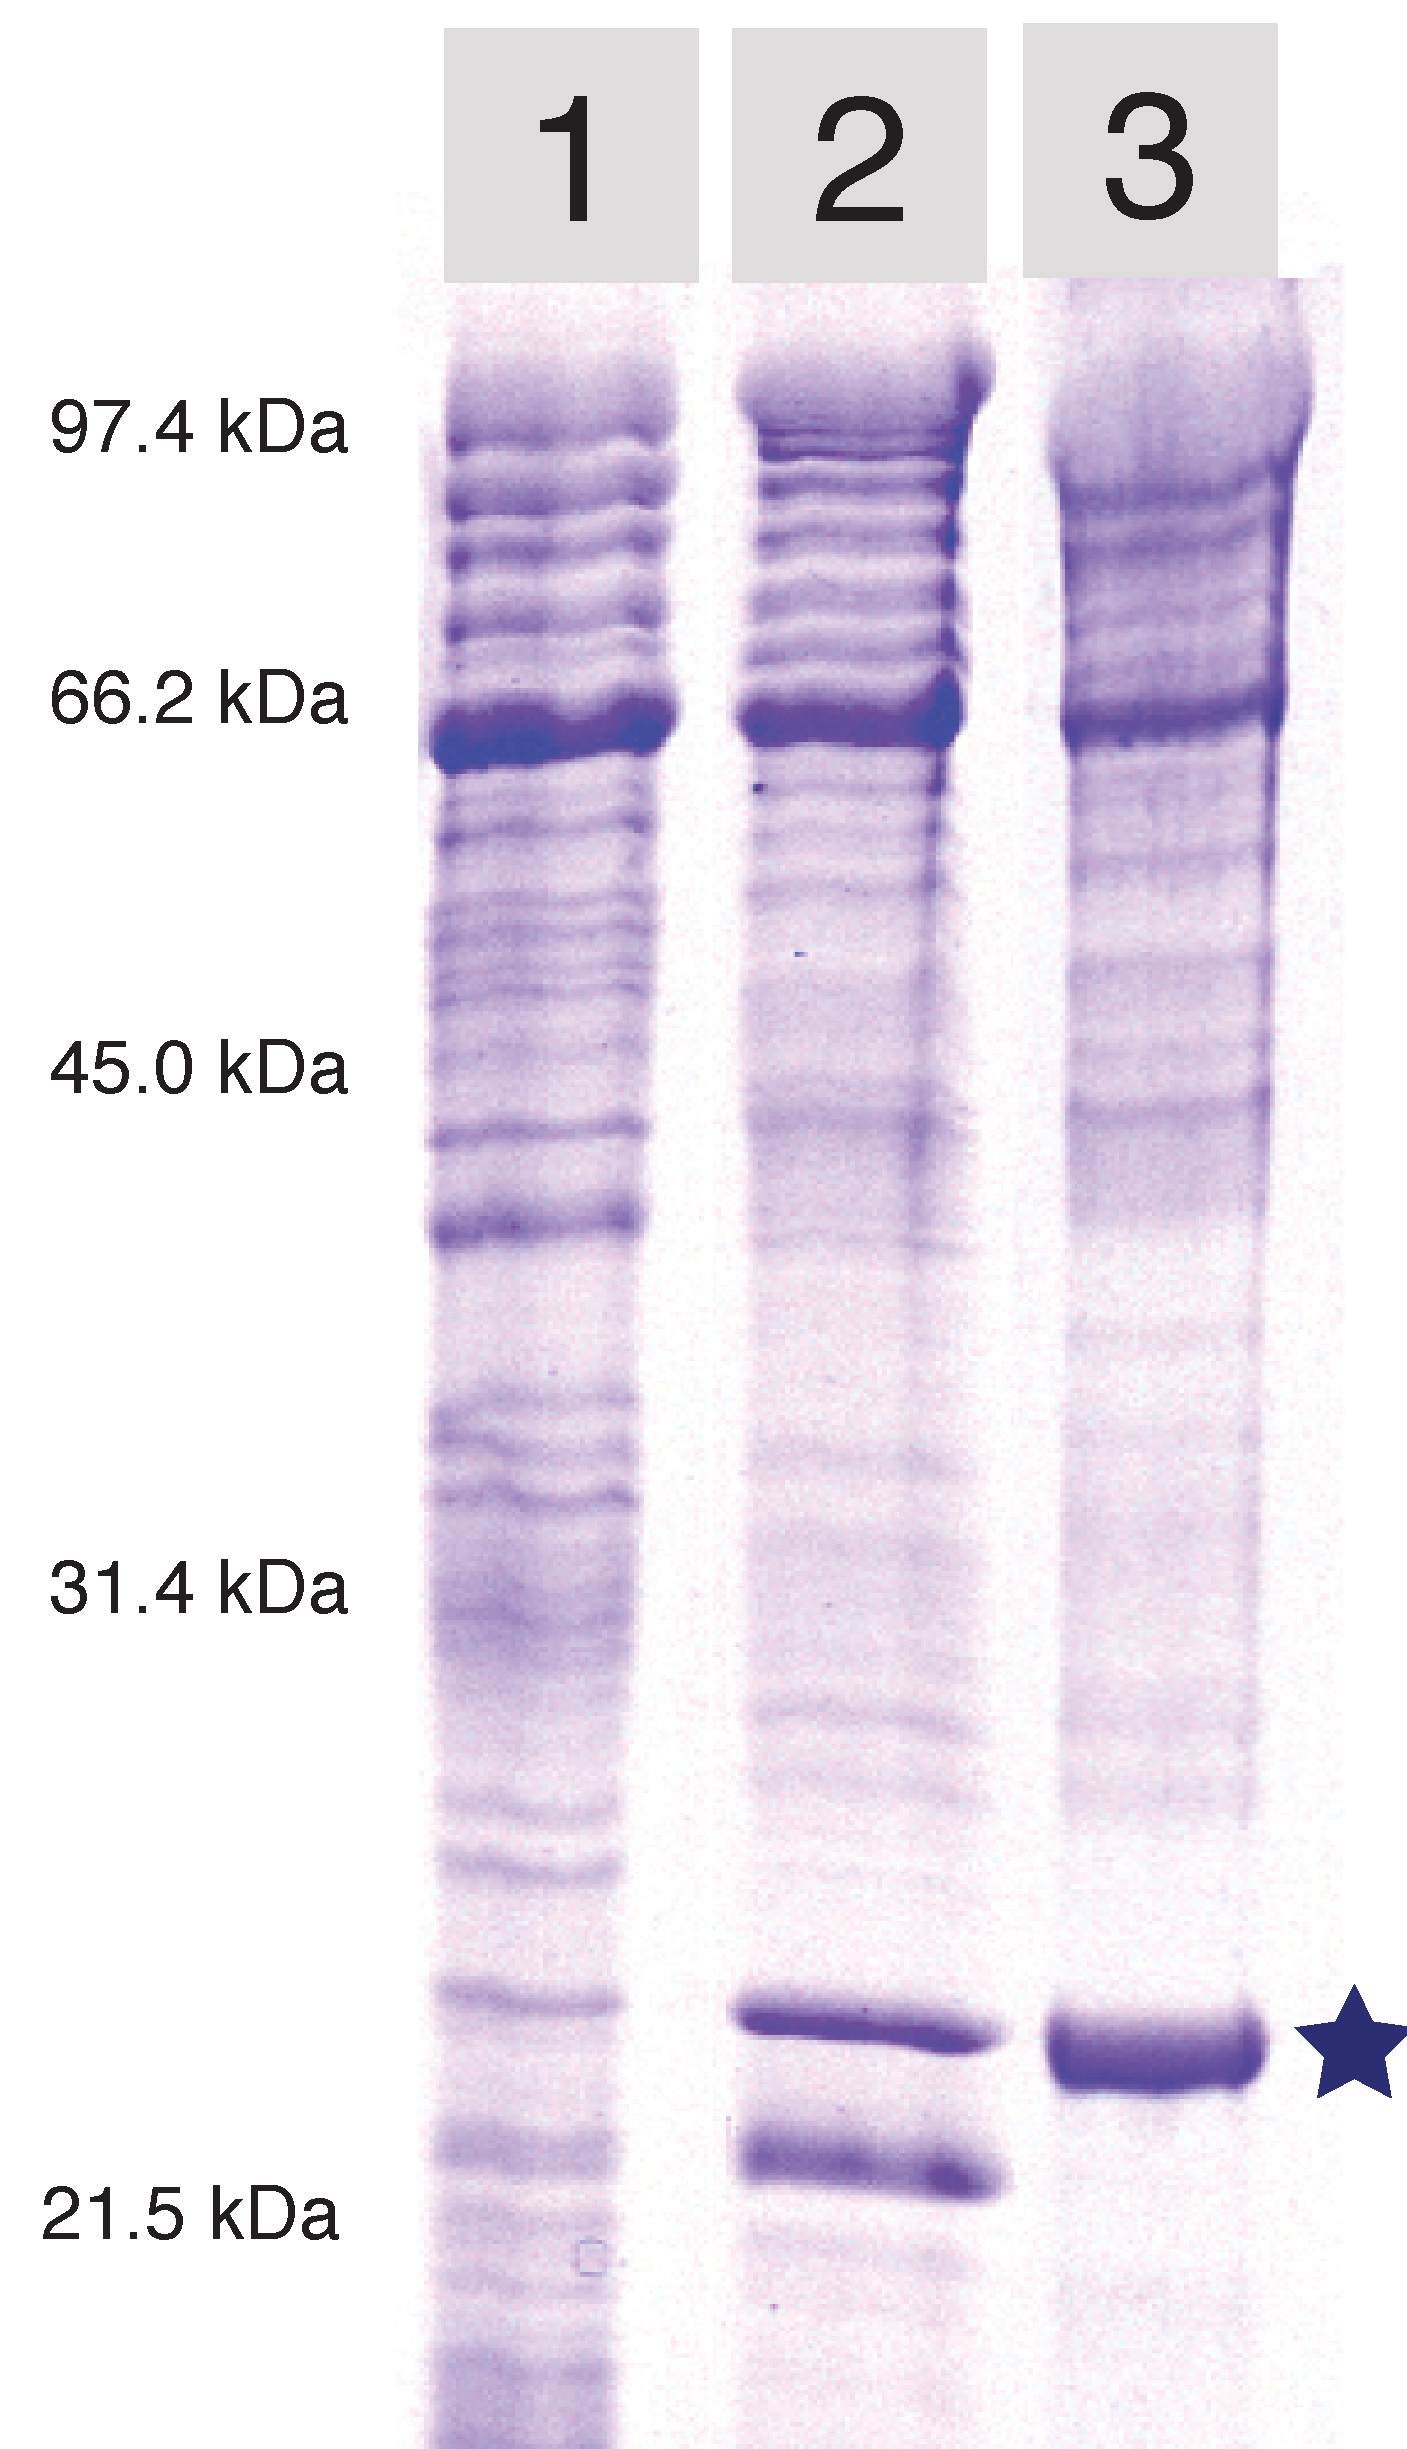
\includegraphics[width=0.2\textwidth]{porin_chapter/img/Fig1-pbsedta.pdf}
   	\end{center}
   	\caption[Coomassie stained \ac{SDS-PAGE} of different protein preparations of \caulobacter.]{
	   	Coomassie stained \ac{SDS-PAGE} of different protein preparations of \caulobacter. 
Lane 1, 7.5 \microlitre of crude membrane preparation. Lane 2, 15 \microlitre of \ac{PBS}-\ac{EDTA} extract, not boiled prior to loading. Lane 3, 15 \microlitre of \ac{PBS}-\ac{EDTA} extract, boiled prior to loading. The star highlights the position of OmpW.
 	}
   	\label{fig:porin-pbsedtagel}
\end{figure}   

\subsection{Identification of channel-forming activity in enriched outer membranes of \textit{C. crescentus}}
The enriched outer membranes were treated with 0.5\% \ac{LDAO}. When small amounts of this detergent solution were added to one or both sides of a black \ac{PC}/n-decane membrane we observed a remarkable increase of membrane conductance indicating that the enriched outer membranes contained membrane-active components. The conductance increase was not sudden, but delayed after addition of the extract. After an initial rapid increase of conductance for 5--10 min, the increase slowed down and saturated at 30--60 min after addition of the detergent solution to the black membranes. It is noteworthy that when the detergent alone was added in the same concentration as with the \ac{PBS}-\ac{EDTA} extracted membranes; it had no influence on the conductance of the lipid bilayer membranes. When the detergent extract of the outer membranes was added at much lower concentrations to the aqueous phase bathing the black lipid membrane, the current increased in a step-wise fashion (see \cref{fig:porin-elutedband}A, upper panel). A histogram of the channel distribution demonstrated that most of the conductance steps had a conductance of about 125 \si{\pico\sievert} in 1M \ce{KCl} (see \cref{fig:porin-elutedband}A, lower panel). Besides the 125 \si{\pico\sievert} channel, some fluctuations with higher conductance (250 and 350 \si{\pico\sievert}) were also obtained which probably represented oligomers of the 125 \si{\pico\sievert} channel that could not be separated at the time scale of our experimental conditions. It is noteworthy that the conductance of these steps was definitely much lower than that of general-diffusion pores from enteric bacteria, which is at least 10 times higher at the same conditions (1--4 \si{\nano\sievert} in 1 M \ce{KCl}\upcite[]{benz1994uptake}). This result suggested that the \ac{PBS}-\ac{EDTA} extracted membranes of \caulobacter contained a porin-like channel of small conductance. 

\subsection{Identification of the channel-forming protein from the enriched outer membranes} 
To identify the protein responsible for the channel-forming activity, the \ac{PBS}-\ac{EDTA} extracted membranes were dissolved in detergent and subjected to preparative \ac{SDS-PAGE}. The gel was cut into thin slices, corresponding to defined molecular mass ranges, and each was eluted overnight with a buffer containing 1\% Genapol. The eluted molecular mass fractions were examined for channel-forming activity in the lipid bilayer assay. Extremely high channel-forming activity was exclusively localized within the molecular mass range around 20 to 22 kDa, corresponding to the protein bands enriched by \ac{PBS}-\ac{EDTA} extraction (see \cref{fig:porin-pbsedtagel}). The other bands from the gel, in particular the 66 kDa band, had no activity in the lipid bilayer assay. When excised and eluted, the band was again subjected to \ac{SDS-PAGE}. Without heating, the gel showed a single protein band of about 20 kDa suggesting that the excised protein was essentially pure (\cref{fig:porin-elutedband}, lane 2). When the excised 20 kDa band was heated to 100\cel prior to addition to \ac{SDS-PAGE}, most of the protein run at an apparent molecular mass of about 22 kDa (\cref{fig:porin-elutedband}, lane 3), with some indication that some of the protein run at 20 kDa (\cref{fig:porin-elutedband}, lane 3). This suggested again that the 20 kDa protein from \caulobacter is heat modifiable.

\begin{figure}[htb]
  	\begin{center}
   		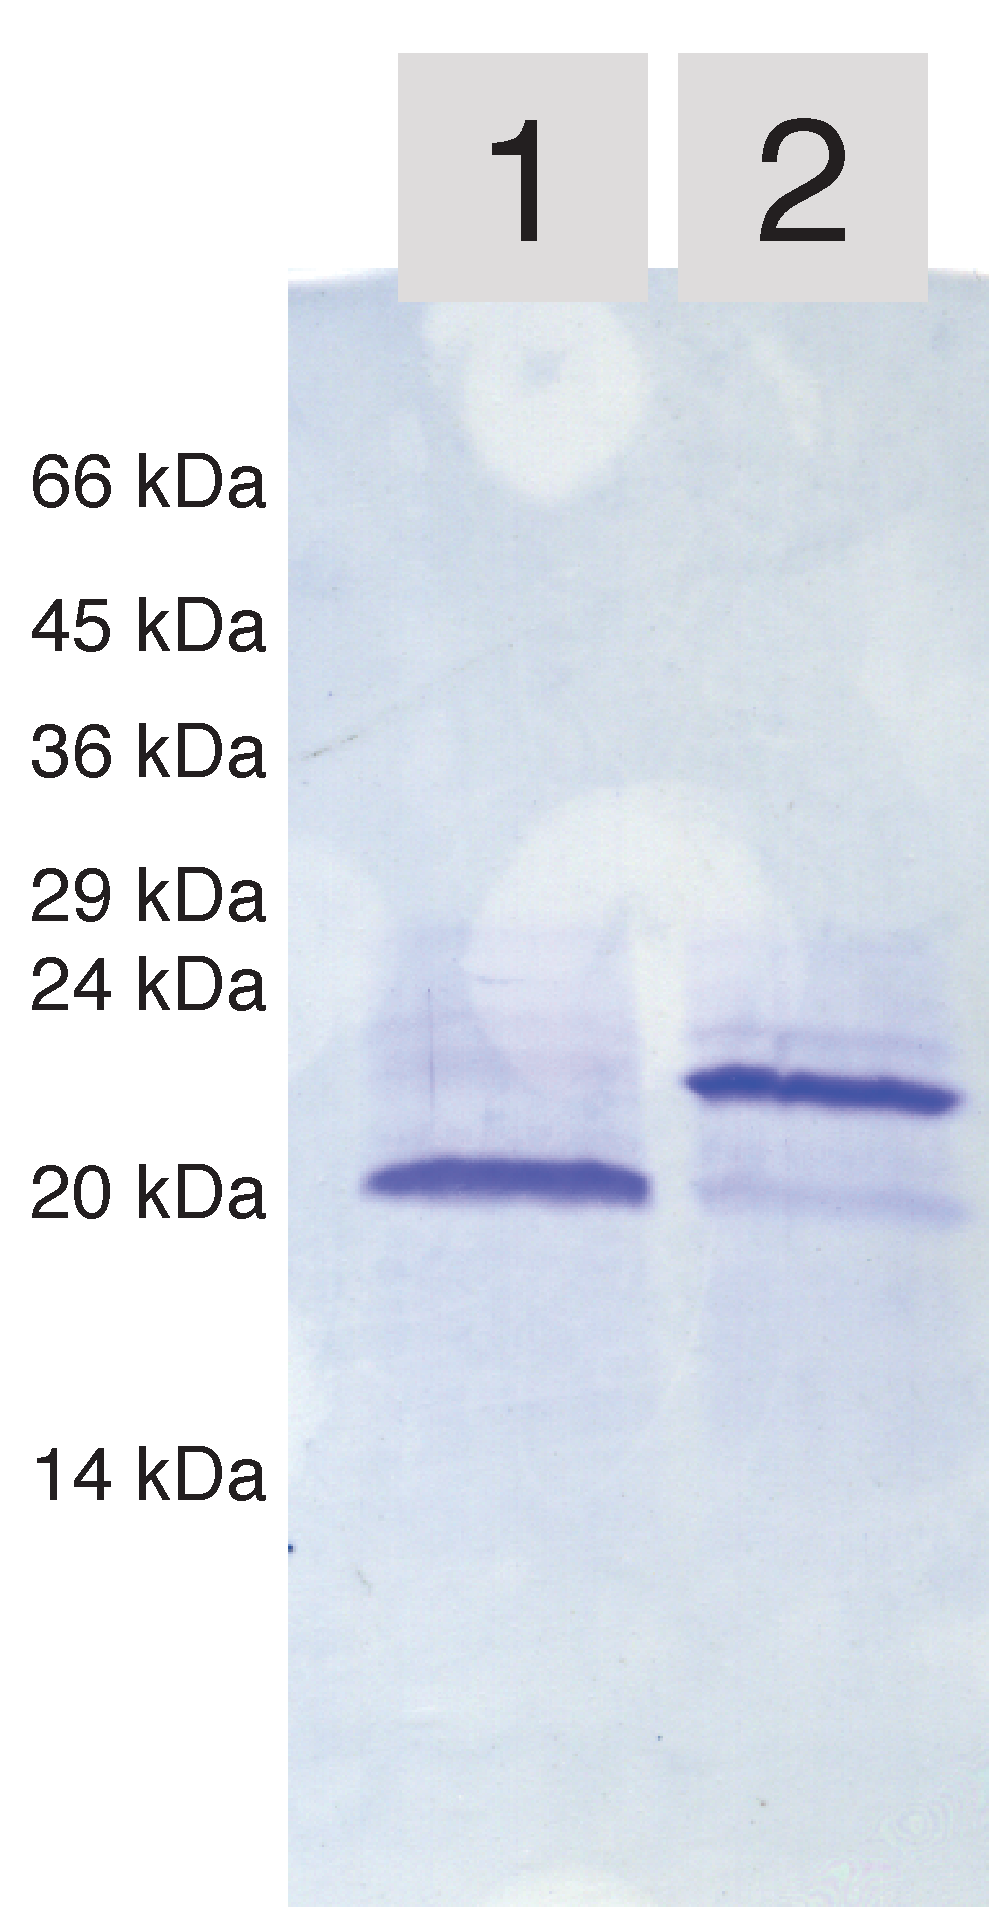
\includegraphics[width=0.2\textwidth]{porin_chapter/img/Fig3-gelpurif.pdf}
   	\end{center}
   	\caption[\ac{SDS-PAGE} showing OmpW from \caulobacter obtained by elution of the 20 kDa band]{
15\% \ac{SDS-PAGE} showing OmpW of \caulobacter obtained by elution of the 20 kDa band from preparative \ac{SDS-PAGE} Lane 1: Molecular mass markers 66 kDa, 45 kDa, 36 kDa, 29 kDa, 24 kDa, 20 kDa, and 14 kDa. Lane 2: 5 \microgram of OmpW solubilized at room temperature for 10 min in 5 \microlitre of sample buffer. Lane 3: 5 \microgram of OmpW solubilized at 100\cel for 10 min in 5 \microlitre of sample buffer. The gel was stained with Coomassie.
   	}
   	\label{fig:porin-elutedband}
\end{figure}   

\subsection{Partial sequencing of the 22 kDa protein of \textit{C. crescentus}}
The 20 kDa protein was subjected to sequencing using Edman-degradation. In a first run the protein could not be sequenced starting from the N-terminus, presumably because of N-terminal blockage. Following trypsin treatment one stretch corresponding to the N-terminal end with a molecular mass of 1764.8 Da could be resolved by sequencing. The sequence of the partial peptide was \texttt{QDFTPNAKGDLIVHAR}, which suggested that the N-terminus was blocked by the formation of pyroglutamate. A \ac{blast} analysis\upcite[]{blast, zhang1997powerblast} of the sequenced peptide unambiguously demonstrated that the 20 kDa protein was OmpW of \caulobacter and was a member of the extensive OmpW-family of outer membrane proteins of Gram-negative bacteria. To ensure that the higher molecular mass band observed in boiled samples was also OmpW; this protein band (about 22 kDa) was also subjected to sequencing following trypsin treatment. Its N-terminal end was identical to that of the 20 kDa protein (OmpW), indicating again that OmpW existed in two different configurations where one was heat-modifiable. 

\subsection{Analysis of the channels formed by OmpW channel-forming protein of \textit{C. crescentus}}

\Cref{fig:porin-20ksinglechannel}B (upper panel) shows a single-channel recording of a \ac{PC} membrane in the presence of the purified OmpW protein of \caulobacter, which was added to a black lipid membrane at a concentration of about 20 \si{\nano\gram\per\milli\litre}. The single-channel recording demonstrates that the protein formed the same defined channels as found in \ac{PBS}-\ac{EDTA} extracted membranes of \caulobacter. The average single-channel conductance was about 125 \si{\pico\sievert} in 1 \si{\molar} \ce{KCl} (almost 40\% of all conductance steps). Only a minor fraction of channels with other conductance was observed (see the histogram in \cref{fig:porin-20ksinglechannel}B, lower panel) suggesting that conductance steps with more than one unit conductance were less frequent for the purified OmpW than for the crude outer membrane fraction. It is noteworthy that the channels formed by OmpW of \caulobacter had a long lifetime, similar to those that have been detected previously for porins of Gram-negative\upcite[]{benz1994uptake} and Gram-positive bacteria\upcite[.]{trias1993characterization, trias1994permeability} All these channel-forming proteins from the cell walls of bacteria form channels in lipid bilayer membranes with long lifetimes at small transmembrane potential (mean lifetime at least 5 min). Furthermore, no voltage-dependence closure was observed in KCl-solution voltages up $\pm$120 mV (data not shown). 

\begin{figure}[p]
  	\begin{center}
   		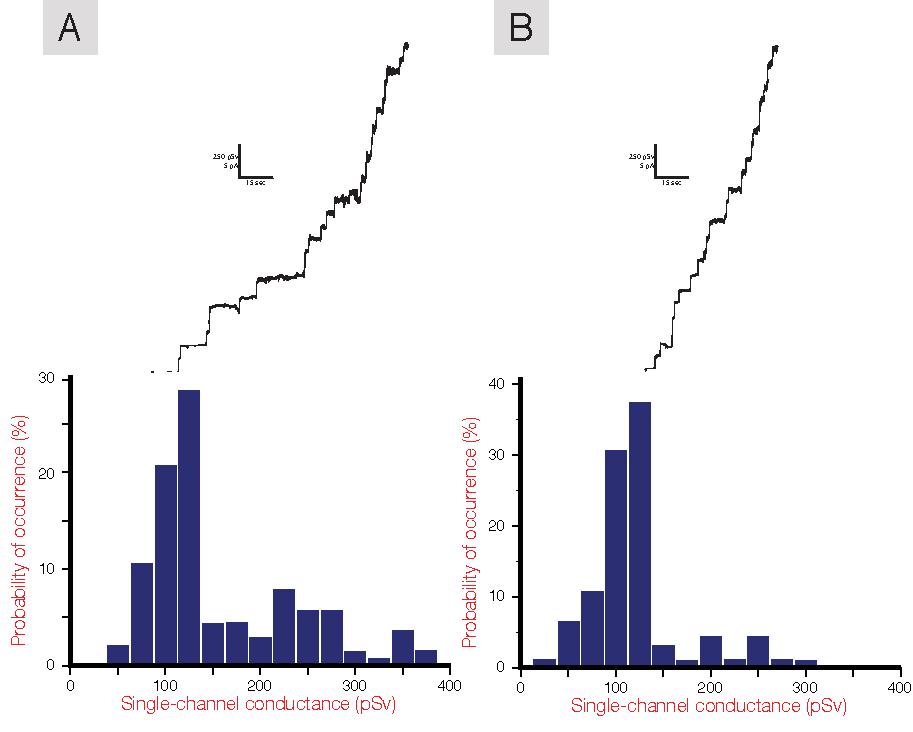
\includegraphics[]{porin_chapter/img/Fig2-singleconductances.pdf}
   	\end{center}
   	\caption[Single-channel measurements with detergent treated outer membrane of C. crescentus and purified 20 kDa protein]{
Single-channel measurements with detergent treated outer membrane of \caulobacter and purified 20 kDa protein.\\
\textbf{A}. Upper panel: Single-channel recording of a PC/n-decane membrane in the presence of enriched outer membranes of \caulobacter. The aqueous phase contained 1 M \ce{KCl} and 100 \si{\nano\gram\per\milli\litre} protein from enriched outer membranes treated with 0.5\% \ac{LDAO}. The applied membrane potential was 20 \si{\milli\volt}; T = 20\cel.\\
Lower panel: Histogram of the probability P(G) for the occurrence of a given conductivity unit observed with membranes formed of \ac{PC}/n-decane in the presence of enriched outer membranes of \caulobacter. P(G) is the probability that a given conductance increment G is observed in the single-channel experiments. It was calculated by dividing the number of fluctuations with a given conductance increment by the total number of conductance fluctuations. The aqueous phase contained 1 M \ce{KCl}. The applied membrane potential was 20 \si{\milli\volt}; T = 20\cel. The average single-channel conductance was 125 \si{\pico\sievert} for 105 single-channel events (left-hand maximum). \\
\textbf{B}. Upper Panel: Single-channel recordings of a \ac{PC}/n-decane membrane in the presence of purified OmpW of \caulobacter. The aqueous phase contained 1 M \ce{KCl} and 20 \si{\nano\gram\per\milli\litre} OmpW dissolved in 1\% Genapol. The applied membrane potential was 20 \si{\milli\volt}; T = 20\cel. \\
Lower panel: Histogram of the probability P(G) for the occurrence of a given conductivity unit observed with membranes formed of \ac{PC}/n-decane in the presence of OmpW of \caulobacter The applied membrane potential was 20 \si{\milli\volt}; T = 20\cel. The average single-channel conductance was 125 \si{\pico\sievert} for 95 single-channel events.
   	}
   	\label{fig:porin-20ksinglechannel}
\end{figure}   

Single-channel experiments were also performed with salts other than \ce{KCl} to obtain information on the size and selectivity of the channels formed by OmpW of \caulobacter. The results are summarized in \cref{tab:porin-conductance}. The conductance sequence of the different salts within the channel was \ce{KCl} $\approx$ \ce{KOAc} $\approx$ \ce{NH4Cl} \textgreater \ce{RbCl} \textgreater \ce{NaCl} \textgreater \ce{CsCl} \textgreater \ce{LiCl}. The influence of cations of different size and mobility on the conductance was quite substantial (see \cref{tab:porin-conductance}) suggesting indeed high cation-selectivity of the OmpW channel. For more bulky cations such as \ce{N(CH3)4+} or the Tris$^+$ cation we observed a very low conductance of much less than 10 \si{\pico\sievert} suggesting that the size of the OmpW channel is indeed very small. 

\begin{table}[htb]
    \centering
    \caption[Average conductance through OmpW]{Average single-channel conductance of OmpW of \caulobacter in different salt solutions and radii, hydrated radii, and limiting molar conductivity of the cations. This data is also presented in a graphical figure, \cref{fig:porin-ionicradii}}
    \label{tab:porin-conductance}
    \begin{tabular}{@{}lrrrrr@{}}
        \toprule
        Salt      & Concentration & Single-channel  & Ion  & Hydrated Ion  & Limiting Molarity     \\ 
              &  &  conductance &  Radius &  Radius &  Conductivity     \\ 
                  & M             & \si{\pico\sievert}        & nm         & nm                  & \si{\milli\sievert\per\molar} \\ \midrule
        \ce{LiCl}      & 1.0           & 15 $\pm$ 3.0                   & 0.059      & 0.216               & 38.68                           \\
        \ce{NaCl}      & 1.0           & 40 $\pm$ 3.5                   & 0.100      & 0.163               & 50.10                           \\
        \ce{KCl}       & 0.01          & 30 $\pm$ 3.2                   & 0.137      & 0.110               & 73.50                           \\
        --\textquotedbl{}--  & 0.03          & 40 $\pm$ 3.4                   &            &                     &                                 \\
         --\textquotedbl{}-- & 0.1           & 55 $\pm$ 4.9                   &            &                     &                                \\
      --\textquotedbl{}-- & 0.3           & 80 $\pm$ 6.2                   &            &                     &                                 \\
        --\textquotedbl{}--  & 1.0           & 125 $\pm$ 8.1                  &            &                     &                                 \\
        --\textquotedbl{}-- & 3.0           & 150 $\pm$ 8.9                  &            &                     &                                 \\
        \ce{NH4Cl}     & 1.0           & 125 $\pm$ 9.5                  & 0.147      & 0.110               & 73.55                           \\
        \ce{RbCl}      & 1.0           & 100 $\pm$ 7.6                  & 0.152      & 0.105               & 77.81                           \\
        \ce{CsCl}      & 1.0           & 30 $\pm$ 2.9                   & 0.167      & 0.106               & 77.26                           \\
        \ce{N(CH3)4Cl} & 1.0           & \textless10                & 0.347      & 0.182               & 44.92                           \\
        \ce{KAcO-} (pH 7)  & 0.1           & 60 $\pm$ 8.0                   &            &                     &                                 \\
         --\textquotedbl{}-- & 1.0           & 125 $\pm$ 10                   &            &                     &                                 \\
        \ce{CaCl2}     & 0.5           & 225 $\pm$ 22                   &            &                     &                                 \\
         --\textquotedbl{}-- & 1.0           & 250 $\pm$ 19                   &            &                     &                                 \\
        \ce{MgCl2}     & 1.0           & 275 $\pm$ 27                   &            &                     &                                 \\ \bottomrule
    \end{tabular}
\end{table}

An additional significant result of the single-channel measurements was the extreme high conductance of OmpW in \ce{CaCl2} (see \cref{tab:porin-conductance}). In 1 M \ce{CaCl2}, the conductance was about 250 \si{\pico\sievert}; this was again close to saturation because in 0.5 M \ce{CaCl2} the conductance was only little lower than in 1 M solution. Interestingly, conductance traces in \ce{CaCl2} solutions were very noisy suggesting a strong interaction between the divalent cations and the OmpW channels. Similarly, channel-forming activity in salt solutions containing divalent cations was much lower than that in monovalent cation solutions, indicating that OmpW could be a channel for divalent cations, such as \ce{Ca^2+} or \ce{Mg^2+}. \Cref{tab:porin-conductance} also shows the average single-channel conductance, G, as a function of the \ce{KCl} concentration in the aqueous phase. Similarly, as in the case of some channels of Gram-positive bacteria\upcite[,]{trias1993characterization, trias1994permeability, riess1998cell} the conductance was not a linear function of the \ce{KCl}-concentration, which means that OmpW did not form a wide, water-filled channel. The saturation with increasing salt concentration could be caused by point net charges and/or a binding site for ions.

\subsection{The OmpW channel of \textit{C. crescentus} is highly cation-selective}

Additional information about the structure of the channel formed by OmpW of \caulobacter was obtained from zero-current membrane potential measurements in presence of salt gradients. A fivefold \ce{KCl} gradient (100 mM versus 500 mM), across a lipid bilayer membrane in which about 100--1000 OmpW channels were reconstituted, resulted in an asymmetry potential of 35 mV at the more dilute side (mean of 3 measurements). This result indicated preferential movement of \ce{K+} ions over \ce{Cl-} through the channel at neutral pH. The zero-current membrane potentials were analyzed using the Goldman-Hodgkin-Katz equation, see \cref{eq:bhk}\upcite[.]{benz1978formation, benz1985ion} The ratio of the potassium permeability, $P_K$, divided by the chloride permeability, $P_{Cl}$, was about 15 (mean of 3 measurements), indicating high cation selectivity of the channel formed by OmpW (see also Discussion, \cpageref{sec:porin-discussion}). This result was confirmed by measurements with \ce{LiCl} and \ce{KOAc}; we observed under the same conditions as for \ce{KCl}, asymmetry potentials around 32 to 35 mV for fivefold gradients, meaning that Pa/Pc was also in these cases also higher than 10. More precise numbers cannot be expected because small errors of the asymmetry potential result in this range in big variations of the permeability ratio Pa/Pc. Size and mobility of the cations did not influence the cation selectivity of OmpW in contrast to the situation observed previously for general diffusion porins\upcite[.]{benz1985ion}
\begin{equation} \label{eq:bhk}
  E_{m,\text{ion}} = \frac{RT}{F} \ln{ \left( \frac{ P_{\text{ion}}[\text{ion}^{+}]_\mathrm{out}}{ P_{\text{ion}}[\text{ion}^{+}]_\mathrm{in}} \right) }
\end{equation}

\subsection{Knocking out ompW removes channel-forming activity} \label{sec:knocking-out-ompw}

To confirm that the gene product encoded by CCNA\_01475 was indeed responsible for the channel forming activity present in our experiments we removed the genomic copy of the gene with a two-step recombination protocol that is standard in \caulobacter genetics. The resulting strain, \caulobacter \del ompW, was confirmed by \ac{PCR} (data not shown) and \ac{SDS-PAGE}. The \ac{SDS-PAGE} analysis of the knockout compared to wild-type can be seen in \cref{fig:porinknockout}. The band that was identified previously as comprising the channel-forming protein was found to be absent in the ompW knockout. Likewise, the channel-forming activity previously found in our extracts was not present in our ompW knockout extracts. These results support the peptide sequencing in that ompW, CCNA\_01475, encodes for an outer membrane porin.

Interestingly, all attempts scale-down our outer membrane extractions, from large flasks to test tubes, were unsuccessful at producing a sample with a prominent \ac{SDS-PAGE} band near 20 kDa (the OmpW band). It is not clear where the important differences are between a flask-based extraction and a tube-based extraction are. A significant amount of time was spent trying to reproduce our original results, seen in \cref{fig:porin-pbsedtagel}, during the time that the knockout was being constructed; culture volume was not considered a significant variable until very late. The reason for this phenomenon is unknown.

All attempts to determine a phenotype for the knockout strain were inconclusive. We hypothesized that the OmpW was involved with \ce{Ca2+} uptake and that without OmpW the cells would have reduced fitness under \ce{Ca2+} limitation. It has previously been shown that \caulobacter does require \ce{Ca2+} in its growth medium, but that Independence from \ce{Ca2+} can be achieved and  `calcium-free' mutants' have been isolated\upcite[.]{smit1992s} All recent attempts to produce growth media without \ce{Ca2+}, in the manner previously published, haven't been successful. It seems that there may be a trace level of calcium contamination of some media components. Nevertheless, no reduction in fitness was observed for our ompW knockout strain compared to wild-type in media replete with \ce{Ca2+} or in media with significantly reduced \ce{Ca2+}. In fact, no \textit{in vivo} phenotype of any kind was observed with our strain \caulobacter \del ompW.

\begin{figure}[htb]
  	\begin{center}
   		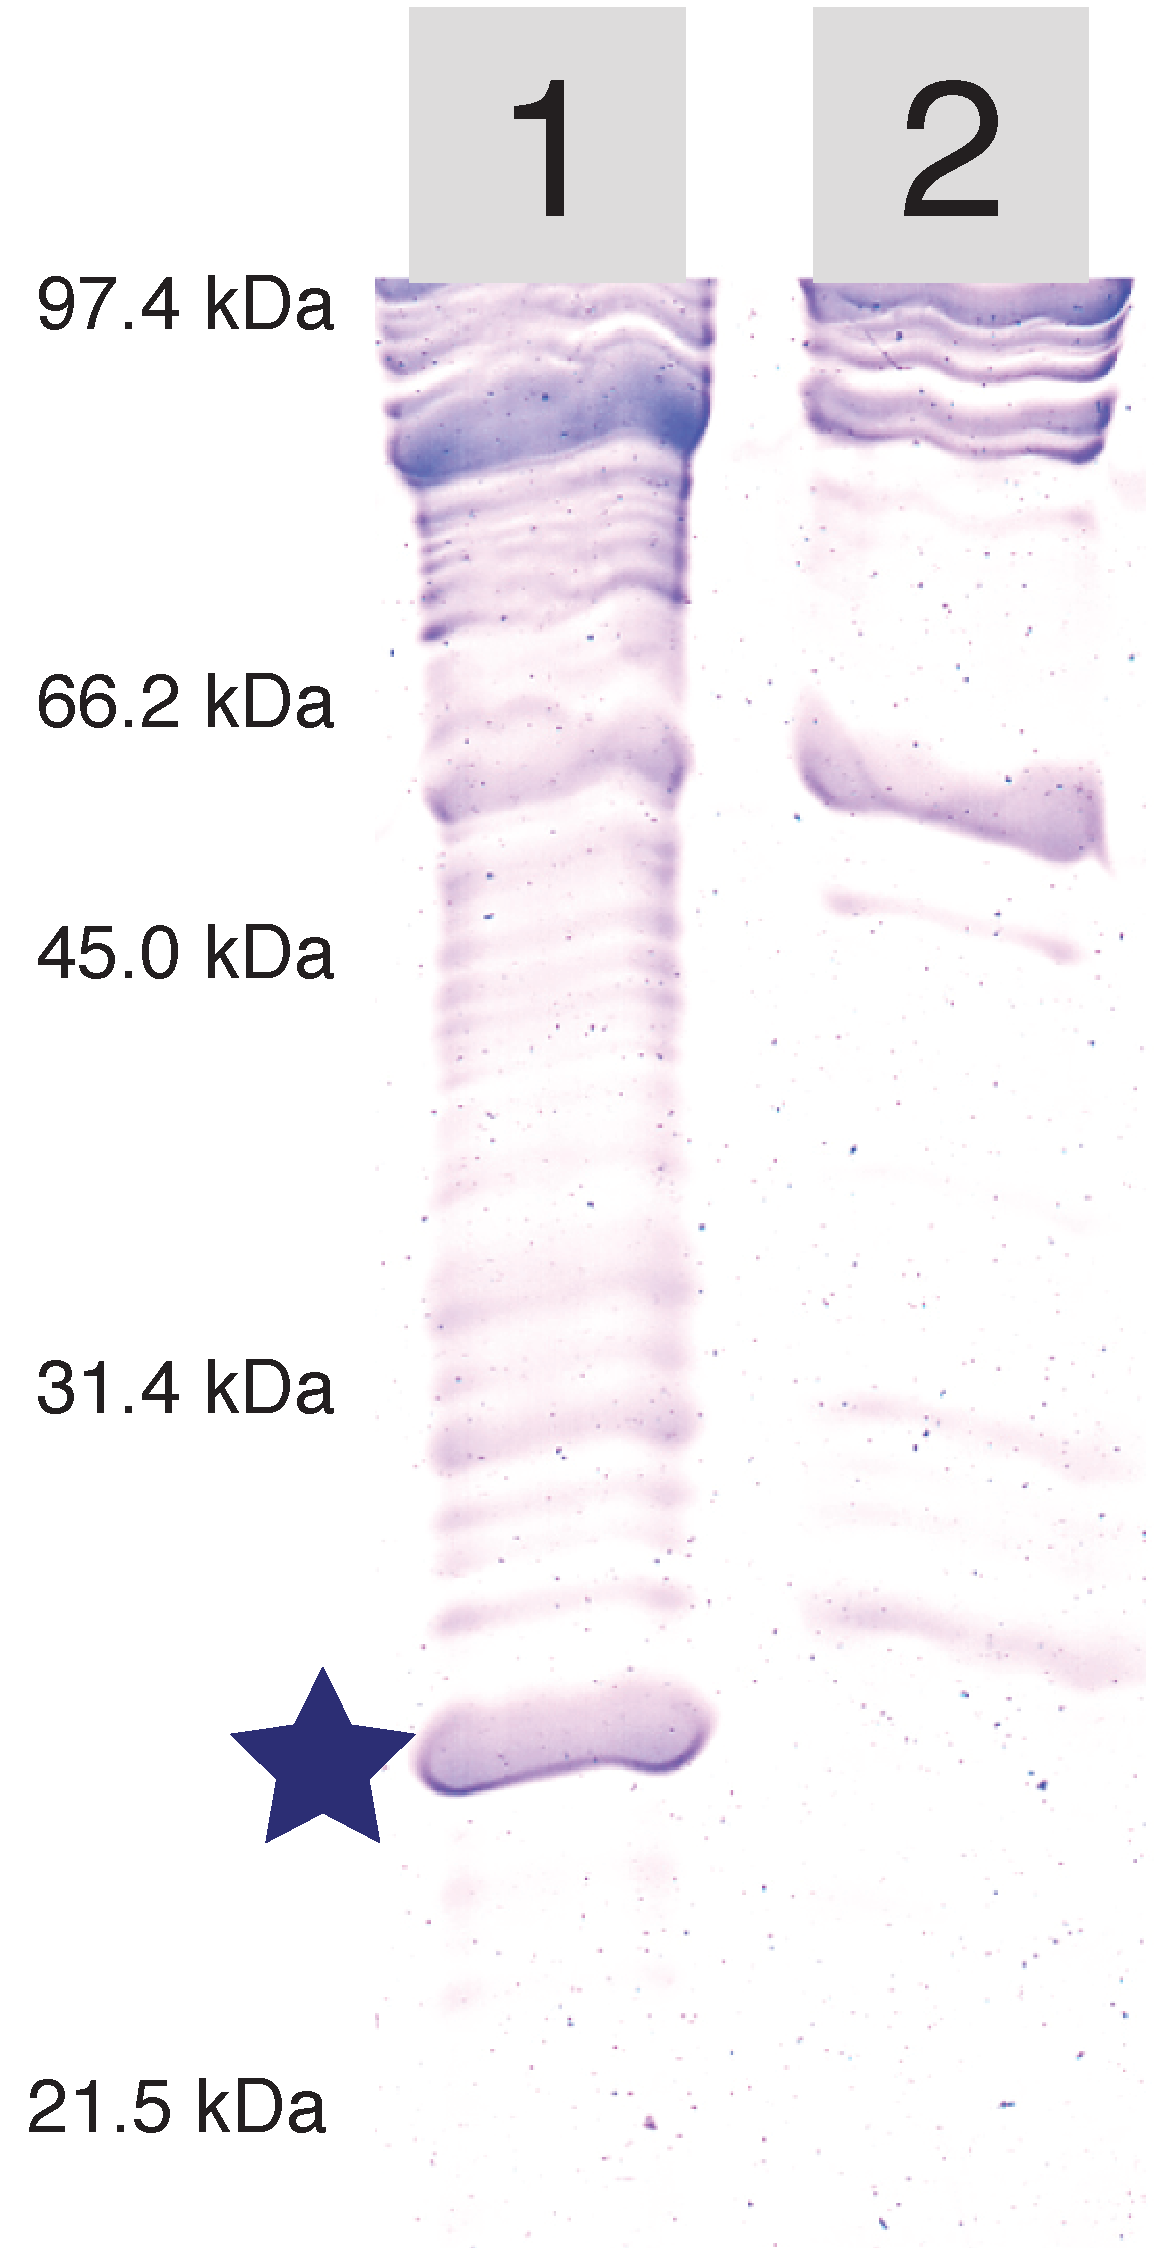
\includegraphics[width=0.2\textwidth]{porin_chapter/img/Fig-knockout.pdf}
   	\end{center}
   	\caption[\ac{SDS-PAGE} of \caulobacter \del ompW]{\ac{SDS-PAGE} analysis of enriched outer membrane preparations of \caulobacter. Lane 1: \caulobacter NA1000. Lane 2: \caulobacter  \del ompW. The star highlights the position of OmpW, the prominent band at 22 kDa. 
   	}
   	\label{fig:porinknockout}
\end{figure}   

\section{Discussion}
\label{sec:porin-discussion}

\subsection{The enriched outer membrane of \caulobacter contains a cation-permeable channel, encoded by ompW}
Here we demonstrated the presence of a channel in the enriched outer membranes of the alpha proteobacterium \caulobacter. Unlike enteric Gram-negatives, the genome does not contain genes that code for the classical outer membrane porins such as OmpC, OmpF, LamB or Tsx\upcite[.]{lohmiller2008tonb, neugebauer2005exbbd, caulobactergenomeseq} Instead the genome of \caulobacter contains 67 genes coding for TonB-dependent receptors\upcite[.]{neugebauer2005exbbd} This suggested that most of the nutrients from the dilute environments where \caulobacter is typically found are actively taken up by TonB-dependent transport systems. Nevertheless, it is clear from this study that \caulobacter also contains an outer membrane channel. The 20 kDa band excised from preparative \ac{SDS-PAGE} had a very high channel-forming activity. No other protein bands excised from gels showed channel-forming activity suggesting that the outer membrane of \caulobacter may contain only one porin-like channel. The channel had a very low single-channel conductance of about 125 \si{\pico\sievert} in 1 M \ce{KCl}. The channel-forming protein was subjected to partial sequencing and was identified as OmpW of \caulobacter. The gene found to encode for the OmpW, CCNA\_01475, was knocked out and the extracts of the resulting strain showed no channel-forming activity.

 The OmpW porin family is widespread amongst Gram-negative bacteria, but with no well established function. Only for OmpW of \ecoli and OprG of \ac{pseudomonas} have channel functions been postulated that may have to do with the uptake of hydrophobic compounds\upcite[.]{hong2006outer, touw2010crystal} In other studies it has been suggested that the channel function of OmpW of \ecoli and OprG of \ac{pseudomonas} may be plugged by W155 and W170, respectively (see \cref{sub:structompw})\upcite[.]{albrecht2006expression, hong2006outer, touw2010crystal} 

Two big-dataset studies out of the Shapiro lab at Stanford University have shed some light on the biology of ompW in \caulobacter; the survey of essential genes by Christen \etal (2011) and the high-throughput analyses of transcription and translation by Schrader \etal (2014). The gene ompW is non-essential for \caulobacter, at least in rich growth medium, \ac{PYE}\upcite[,]{christen2011essential} The gene lies on the forward strand of the genome surrounded by genes of seemingly unrelated function. It is transcribed on to a monocistronic mRNA, while the preceding and succeeding genes are both transcribed on separate polycistronic mRNAs\upcite[.]{schrader2014coding}) The ompW gene is not highly transcribed, nor translated in either rich medium (\ac{PYE})) nor limiting medium (M2G), but interestingly the gene is transcribed at a much higher rate relative rate in rich media than in limiting media while its translation rate remains relatively equal in both media. The differences in transcription rate and translational efficiency between media types was relatively small within to entire study by Schrader \etal, and so it wasn't focused on or discussed in the original study. The reduction in transcriptional activity in minimal medium suggests some transcriptional control, but the translation rate (as measured by ribosome footprinting RNA-seq) remained relatively unchanged (0.9 vs. 0.8 ribosomes per kilobase per million-reads) suggesting that the changes in transcription maybe superseded by a translational control mechanism.

\subsection{Properties of OmpW in the \textit{C. crescentus} outer membrane}
OmpW of \caulobacter was found to be highly cation-selective. Its selectivity for \ce{K+} ions over \ce{Cl-} was at least 10-fold; the calculated value was about 12. However, it has to be kept in mind that the permeability ratio Pa/Pc reacts in this range very sensitive to small changes of the asymmetry potential\upcite[.]{benzhancock1987mechanism} This means that we found little indication for the permeation of anions through OmpW because the single channel conductance in 1 M \ce{KCl} was the same as in 1 M \ce{KOAc}, despite the fact that chloride in the aqueous phase has a much higher mobility than acetate. In addition, the single channel conductance was not a linear function of the bulk aqueous salt concentration, see \cref{tab:porin-conductance}. Instead the conductance showed strong saturation; at 3 M \ce{KCl} conductance was only slightly higher (150 \si{\pico\sievert}) than at 1 M \ce{KCl} (125 \si{\pico\sievert}). Similarly, at 0.3 M \ce{KCl}, conductance was only little smaller (80 \si{\pico\sievert}) than at 1 M \ce{KCl}. Experiments with different alkaline cations indicated clearly that OmpW does not form an aqueous pore, which would be typical for most Gram-negative and Gram-positive bacterial porins, even if they contained point charges\upcite[.]{benz1994uptake, riess2000discovery} Instead OmpW of \caulobacter appeared to be an ion channel; its single channel conductance had a maximum for ammonium and potassium ions and became much smaller for bigger cations indicating that they likely loose part of their hydration shell while moving through the channel. This argues for a small selectivity filter inside the channel. Presumably, the ionic radii of the different cations and not the sizes of their hydration shells, play an important role for their permeation through OmpW as \cref{tab:porin-conductance} clearly indicates. \Cref{fig:porin-ionicradii} shows the single channel conductance of OmpW as a function of the ionic radii of the ions\upcite[.]{pauling1960nature, shannon1976revised, smirnov1997ammonium} The conductance data for another small substrate-specific channel (LamB of \ecoli) is given for comparison\upcite[.]{benz1987mechanism} The relationship for OmpW follows approximately the Eisenman series VI for carrier-mediated transport of cations or for the transport of monovalent cations through channels\upcite[.]{eisenman1983ionic} This means presumably that the field strength inside the channel is presumably medium-sized. Ion transport trough general diffusion channels of enteric bacteria follow instead Eisenman series I or II indicating low field strength in the channels. The minimum diameter of OmpW is presumably close to that of \ce{Cs+} or smaller than that of \ce{N(CH3)4+} ions because larger organic cations have a very low permeability through OmpW, if any. 

\begin{figure}[htb]
  	\begin{center}
   		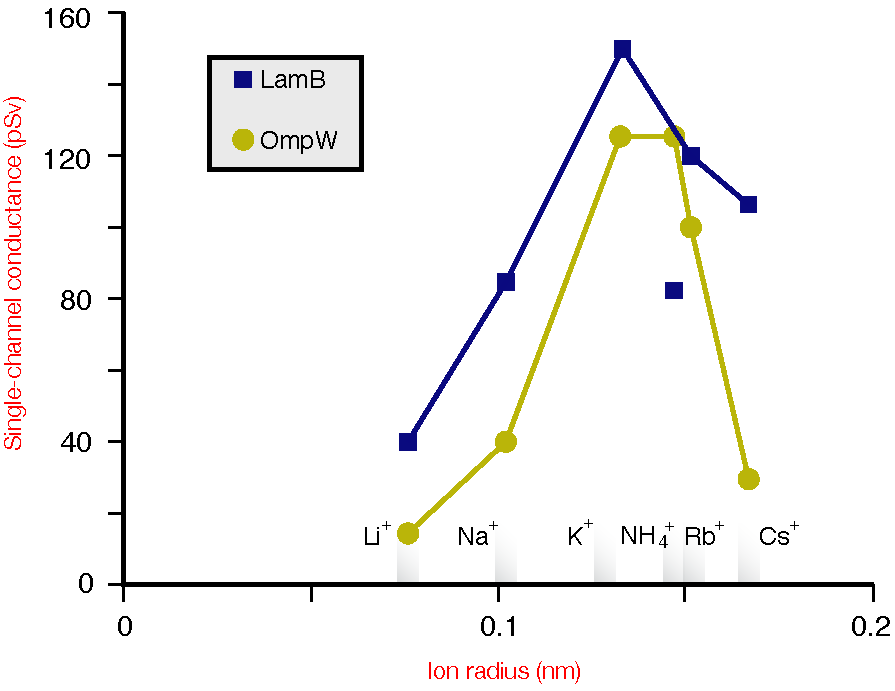
\includegraphics[]{porin_chapter/img/Fig4-conductancegraph.pdf}
   	\end{center}
   	\caption[Single-channel conductance of OmpW in 1 M salt solution as a function of the ionic radii of monovalent cations]{
Single-channel conductance of OmpW in 1 M salt solution as a function of the ionic radii of monovalent cations. 
The data were taken from \cref{tab:porin-conductance}. The single-channel conductance through LamB of \ecoli is given for comparison (data taken from \fullcite{benz1986pore}).
   	}
   	\label{fig:porin-ionicradii}
\end{figure}   

OmpW of \caulobacter clearly functions as a cation-permeable channel, having a preference for divalent cations, since calcium and magnesium ions had a higher permeability through OmpW than potassium ions. This could indeed mean that it is a channel for the transport of calcium and/or magnesium ions. It is noteworthy that such a function has not previously been established for OmpW. The reason for this is that OmpW is a rather small channel with only eight beta strands and so has little possibility for the passage of solutes. Previous data from structural studies of OmpW of \ecoli and OprG of \ac{pseudomonas} suggested that members of the OmpW family could be involved in the transport of small hydrophobic molecules across the bacterial outer membrane\upcite[.]{hong2006outer, touw2010crystal} It is also possible that they are blocked\upcite[.]{albrecht2006expression} Lipid bilayer experiments with OmpW of \ecoli suggested that it forms small ion-permeable channels with a conductance of about 20 \si{\pico\sievert} in 1 M \ce{KCl}\upcite[,]{hong2006outer} which is considerably lower than that of \caulobacter OmpW. The 3-D structure of \ac{pseudomonas} OprG, another member of the OmpW family, was resolved at 2.4 \AA resolution\upcite[.]{touw2010crystal} Again the structure suggested that OprG forms a channel for the diffusion of small hydrophobic molecules, although lipid bilayer experiments proposed a single-channel conductance of about 500 \si{\pico\sievert} for OprG\upcite[.]{mcphee2009major} This means that OmpW of \caulobacter forms a channel that has, despite sequence homologies with OmpW of \ecoli and OprG of \ac{pseudomonas} (see below), a completely different function than other outer membrane proteins.

\subsection{Structure of OmpW of \textit{C. crescentus}}\label{sub:structompw}
Sequence comparison, \ac{blast}, of OmpW of \caulobacter with other members of the OmpW family suggested that it had highest homology with OmpW of \textit{Caulobacter segnis} ATCC 21756, \textit{Asticcacaulis excentricus} CB 48, \textit{Brevundimonas} sp. BAL3, and \textit{Phenylobacterium zucineum} HLK1\upcite[.]{blast, zhang1997powerblast} These bacteria are closely related to the genus \textit{Caulobacter}, belonging to the family \textit{Caulobacteraceae}, order \textit{Caulobacterales}. All these OmpW polypeptides are similar in length to \caulobacter OmpW (200 to 250 amino acids) and share many strategically positioned conserved residues. The homology of the \caulobacter OmpW to the OmpW proteins with known 3D structure (OmpW of \ecoli and OprG of \ac{pseudomonas}) is less pronounced, but still obvious (amino acid identity is approximately 32\% in both cases and and 19.4\% for all three proteins  (Hong et al., 2006; Touw et al., 2010). 41 amino acids, including many glycines and several prolines, appear to be highly conserved between all three OmpW family proteins. This allows a meaningful comparison between the three different OmpW species (see \cref{fig:porin-seqalign}) and it is also possible to built the possible structural model of OmpW of \caulobacter using homology modeling approach\upcite[]{eswar2008protein} (see below). 

\begin{figure}[htb]
  	\begin{center}
   		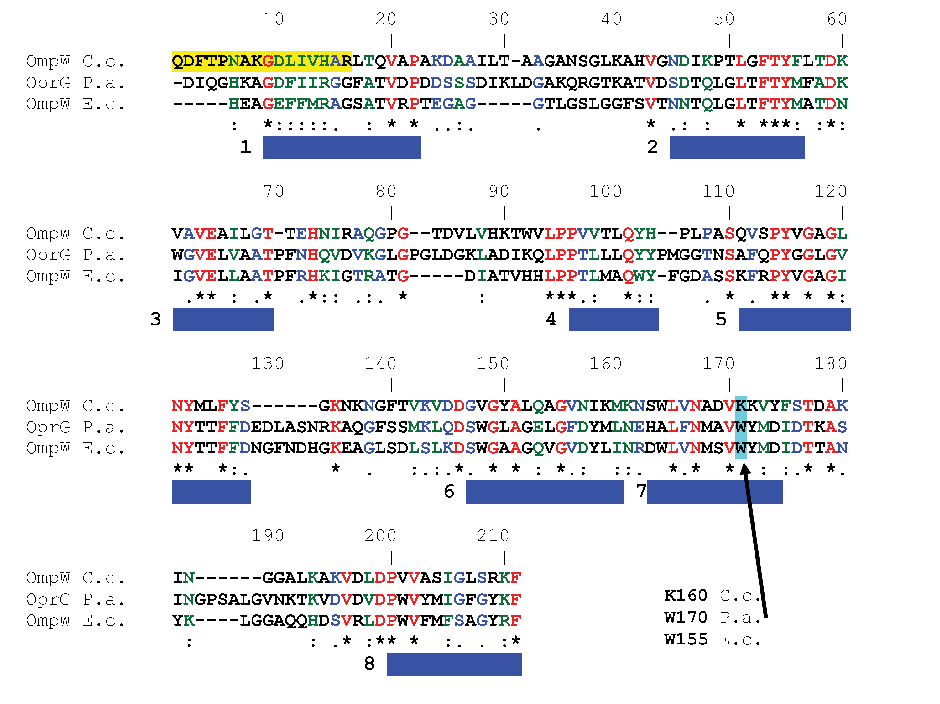
\includegraphics[]{porin_chapter/img/Fig5-seqalign.pdf}
   	\end{center}
   	\caption[Amino acid sequence alignment of OprG of \ac{pseudomonas}, OmpW of \ecoli, and OmpW of \caulobacter]{Amino acid sequence alignment of OprG of \ac{pseudomonas}, OmpW of \ecoli, and OmpW of \caulobacter.
The alignment was performed using Pole Bioinformatique Lyonnaise Network Protein Sequence Analysis (\url{http://npsa-pbil.ibcp.fr}). Amino acids identical in all three proteins are highlighted in red, strongly similar amino acids (:) are given in green and weakly similar ones (.) in blue. The replacement of W155 of OmpW of \ecoli and W170 of OprG of \ac{pseudomonas} by K160 of \caulobacter is given in green color and is indicated by an arrow. The eight beta strands in OprG of \ac{pseudomonas} and in OmpW of \ecoli are numbered and indicated by blue bars. The yellow highlighted sequence was found by N-terminal sequencing of OmpW of \caulobacter.
   	}
   	\label{fig:porin-seqalign}
\end{figure}   

Crystal structures of \ecoli OmpW\upcite[]{hong2006outer} and \ac{pseudomonas} OprG\upcite[]{touw2010crystal} suggested the formation of hydrophobic channels for these proteins and they are believed to be responsible for the passage of hydrophobic solutes across the bacterial outer membrane. Small and hydrophobic \ecoli OmpW channel has a conductance of approximately 20 \si{\pico\sievert} in 1 M \ce{KCl}\upcite[.]{hong2006outer} In contrast, the \caulobacter OmpW formed a channel with a relatively high conductance of 125 \si{\pico\sievert} in 1 M \ce{KCl} in our bilayer measurements. A comparison of the structures of these OmpW family proteins revealed factors that might lead to a larger conductance in \caulobacter OmpW. Crystal structures suggested that both \ecoli OmpW and \ac{pseudomonas} OprG form a hydrophobic gate (\cref{fig:porin-models}A; b and c) in the central region of the channel. Both channels have an aromatic, bulky and hydrophobic tryptophan residue as a part of a hydrophobic gate, which may make the passage of ions through channels difficult. Similarly, W155 of OmpW of \ecoli\upcite{hong2006outer} and W170 of OprG of \ac{pseudomonas}\upcite[,]{touw2010crystal} which are both considered as plugs of the channels are replaced in OmpW of \caulobacter by K160. This may indicate that this channel has a function different from that of the homologs in \ecoli and \ac{pseudomonas} In addition, \caulobacter OmpW has a hydrophilic and relatively less bulky lysine residue at the corresponding position (\cref{fig:porin-models}A; a), which is unlikely to hinder passage of ions through the channel. In addition, the \caulobacter OmpW has a relatively more hydrophilic interior environment of the channel (\cref{fig:porin-models}A; a), as shown by green color surface within the black box) as compared to the \ecoli OmpW (\cref{fig:porin-models}; b) and the  \ac{pseudomonas} OprG (\cref{fig:porin-models}; c). For \ecoli OmpW and \ac{pseudomonas} OprG the interior surface of the channel is hydrophobic (white color surface), which could make the permeation of ions through the channel energetically unfavorable. \caulobacter OmpW, on the other hand, due to its relative hydrophilic environment may not provide the permeation barrier to ion passage, resulting in a relatively higher conductance of the channel. 

\begin{figure}[htb]
  	\begin{center}
   		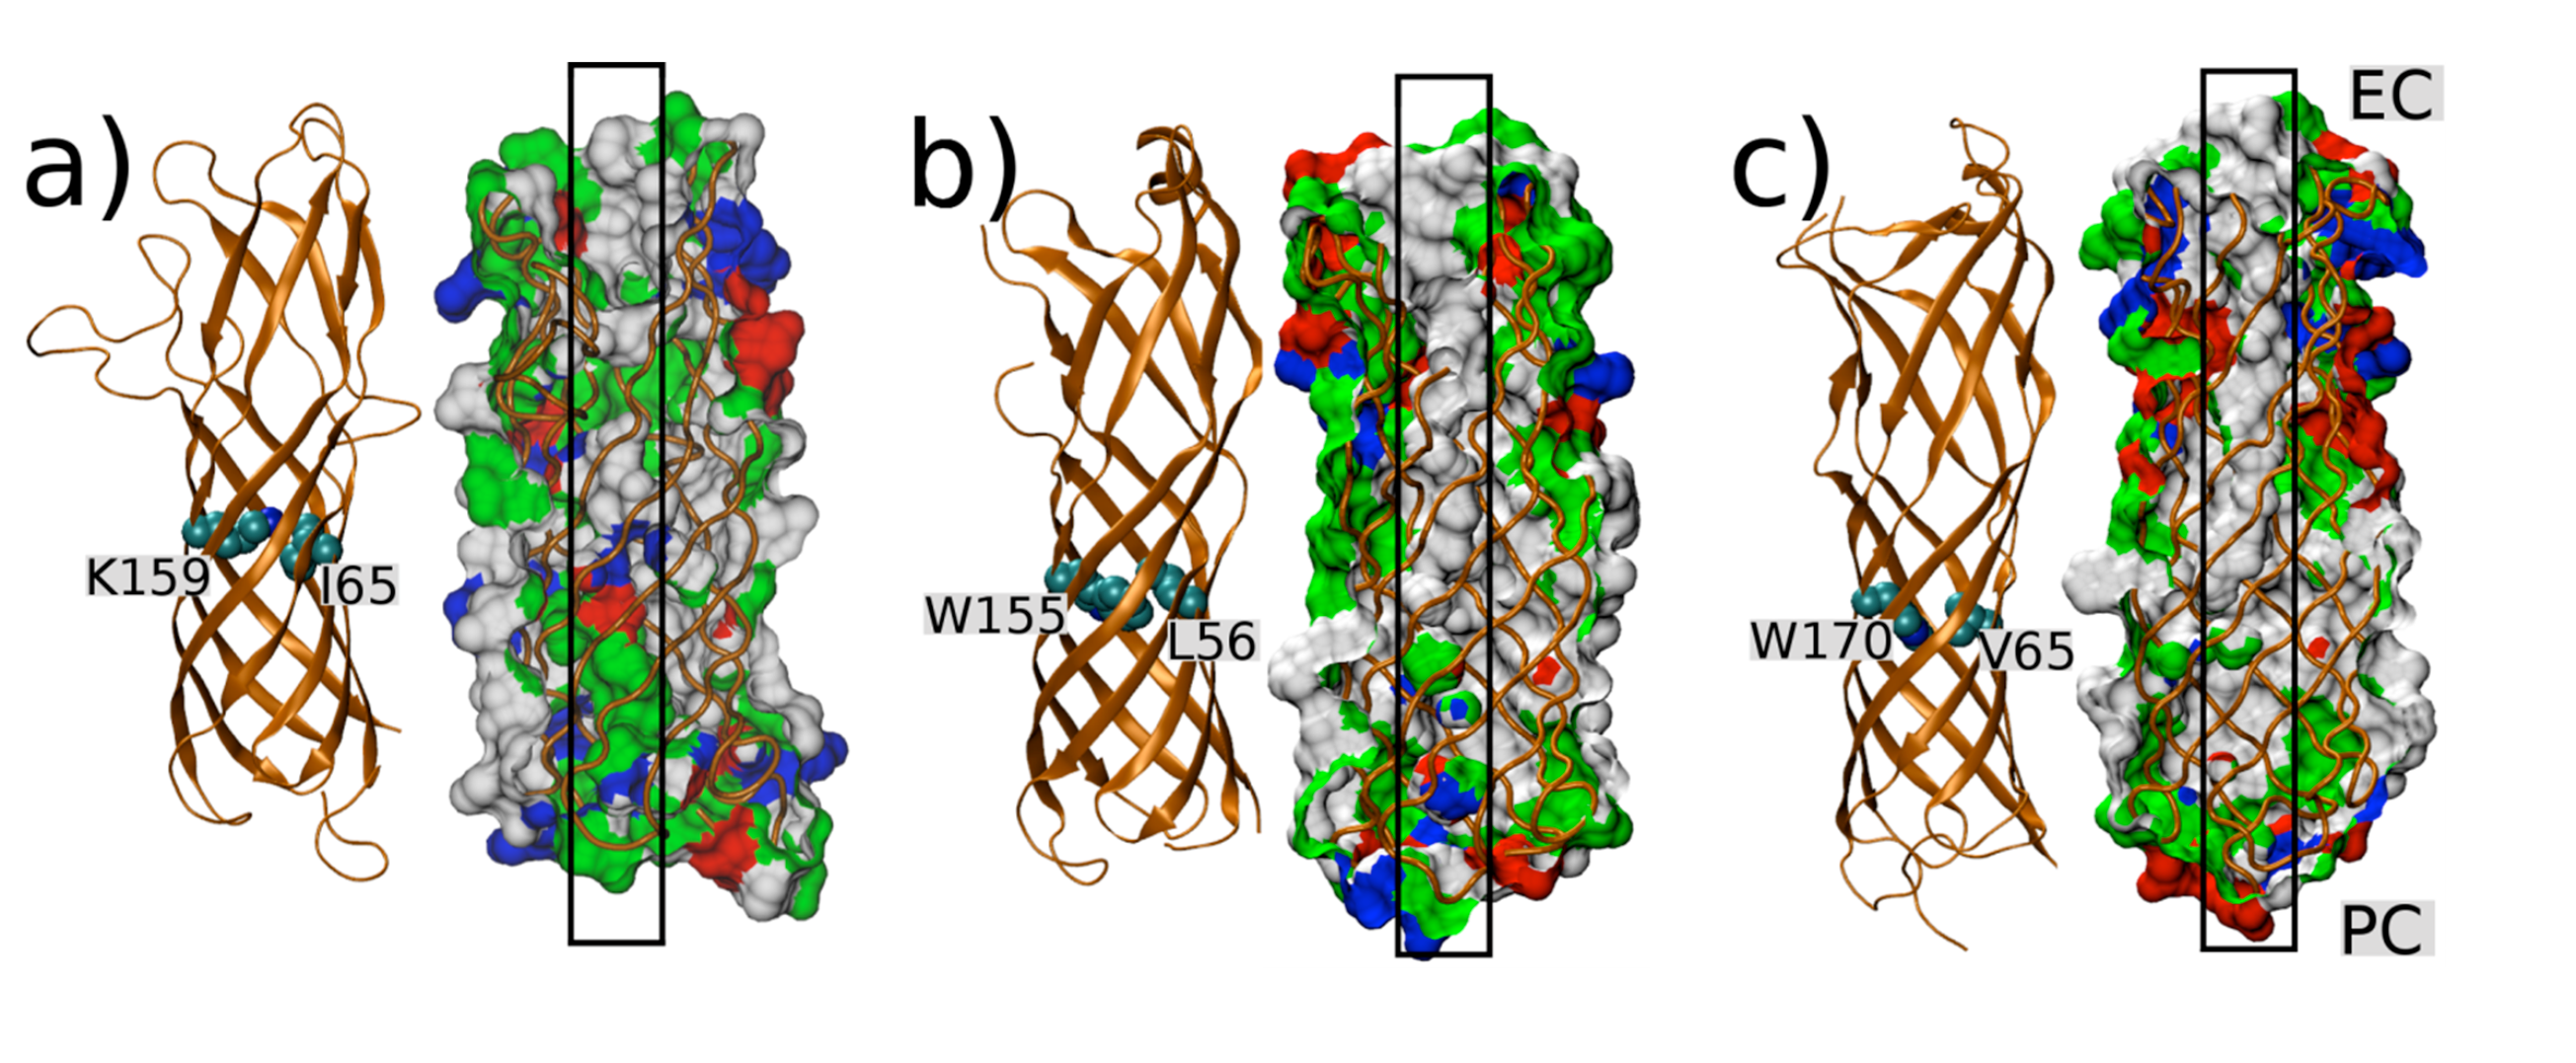
\includegraphics[width=\textwidth]{porin_chapter/img/Fig6a-models.pdf}
   	\end{center}
   	\caption[Structural properties of OmpW of \caulobacter]{
      Comparison of structural features between a) OmpW \caulobacter b) OmpW \ecoli c) OprG \ac{pseudomonas}. Residues, which are a part of a putative hydrophobic gate in \ecoli (W155 and L56) and \ac{pseudomonas} (W170 and V65) channels are shown as spheres. Corresponding residues in OmpW \caulobacter (K159 and I65) are also shown. Additionally all the channels are shown as a surface representation and color coded according to residue type (Green: hydrophilic, white: hydrophobic, red: acidic, blue: basic). Channels are cut from the front to enable visualization of interior channel surface. Black colored box indicate a putative ion transport pathway across the channel. EC and PC denote extracellular and periplasmic sides of the channel respectively.
   	}
   	\label{fig:porin-models}
\end{figure}   

\begin{figure}[htb]
  	\begin{center}
   		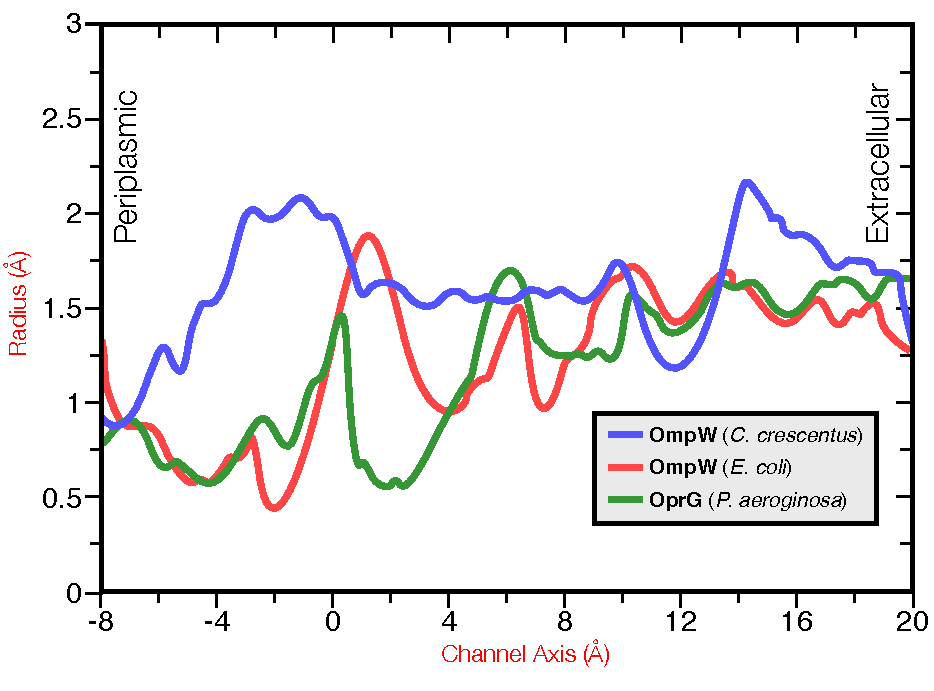
\includegraphics[]{porin_chapter/img/Fig6-poresizes.pdf}
   	\end{center}
   	\caption[Comparison of porin channel radii]{
Comparison of channel radii between \caulobacter OmpW (blue), \ecoli OmpW (red) and OprG of \ac{pseudomonas} (green) along the channel axis. The channel radii were calculated using the program \texttt{HOLE} (\fullcite{smart1996hole}). The extracelluar side is indicted along the right side and the periplasmic side is indicated along the left side.
   	}
   	\label{fig:porin-poresizes}
\end{figure}   

We also examined the contribution of the size of the pore towards higher conductance of \caulobacter OmpW. We observed a slightly larger radius of \caulobacter OmpW channel as compared to other two channels in several regions, particularly from the center of the channel towards the periplasmic side (\cref{fig:porin-poresizes}). Another important feature of the OmpW family channels from \ecoli and \ac{pseudomonas} is the presence of a lateral opening in the barrel wall, which is suggested to allow diffusion of small hydrophobic solutes across the outer membrane by a lateral diffusion mechanism\upcite[.]{hong2006outer, touw2010crystal} In our modeled structure of \caulobacter OmpW, we do not observe such an opening in the channel which further supports the view that the \caulobacter channel may have a different function from that of \ecoli OmpW and \ac{pseudomonas} OprG. Interestingly, the structure of OprG shows additional short beta-strands (not shown in \cref{fig:porin-seqalign}) that are not membrane spanning. These beta-strands seem to extend over the thickness of the outer membrane, which means that they form long external loops\upcite[.]{hong2006outer, touw2010crystal} The solved structures OmpW from \ecoli and OprG from \ac{pseudomonas} provide examples of  successful crystallization efforts for this class of protein and they are exciting starting points for future work towards improving the structural knowledge of OmpW from \caulobacter.

\caulobacter has a requirement for calcium, though it is not clear where the absolute requirement lies. \ce{Ca^2+} ions are needed for assembly of the crystalline \ac{S-layer} RsaA\upcite[.]{nomellini1997factors}. Since RsaA is secreted by a type I secretion mechanism, it is likely that calcium is also needed for either secretion or folding of the protein following secretion, in a manner analogous to all other type I secreted proteins.  However, the \ac{S-layer} a completely dispensable structure. Moreover, the type 1 secretion apparatus spans both the cytoplasmic and outer membranes; hence for \ac{S-layer} there is no apparent need for a channel that enables \ce{Ca^2+} ion movement to the periplasm. There are, however, additional still undefined roles for \ce{Ca^2+} ions. Mutants no longer requiring calcium compounds for growth can be isolated\upcite[.]{walker94} One consequence of all these mutants is the loss of the \ac{OPS} of \ac{LPS} that is used for \ac{S-layer} attachment. As a consequence, these so called `calcium-independent' mutants all shed RsaA into the culture medium. This causal relationship has not been deciphered, but since \ac{OPS} biosynthesis involves synthesis activities within the periplasmic space, it may be that a calcium selective OmpW porin plays a specific role in this process. Here we have provided clear evidence that OmpW could be responsible for the uptake of cations, especially divalent cations, like \ce{Ca2+} in \caulobacter. 


%    3. Notes
%    4. Footnotes
%    5. Bibliography
% prints author names as small caps
	\renewcommand{\mkbibnamefirst}[1]{\textsc{#1}}
	\renewcommand{\mkbibnamelast}[1]{\textsc{#1}}
	\renewcommand{\mkbibnameprefix}[1]{\textsc{#1}}
	\renewcommand{\mkbibnameaffix}[1]{\textsc{#1}} 
	\printbibliography[heading=bibintoc]  %% This actually makes the bibliography %%

\appendix
%    6. Appendices (including copies of all required UBC Research
%       Ethics Board's Certificates of Approval)
%	\include{reb-coa}	% pdfpages is useful here

\chapter*{Appendix}
% \section{The amino aid sequence of RsaA from \caulobacter}
\begin{figure}[htb]
  	\begin{center}
\label{app:rsaseq}
\texttt{\singlespacing\small\underline{MAYTTAQLVTAYTNANLGKAPDAATTLTLDAYATQTQTGGLSDAAALTNTLKLVNSTTAV}\hfill-60~~\\
\underline{AIQTYQFFTGVAPSAAGLDFLVDSTTNTNDLNDAYYSKFAQENRFINFSINLATGAGAGA}\hfill-120~\\
\underline{TAFAAAYTGVSYAQTVATAYDKIIGNAVATAAGVDVAAAVAFLSRQANIDYLTAFVRANT}\hfill-180~\\
\underline{PFTAAADIDLAVKAALIGTILNAATVSGIGGYATATAAMI}NDLSDGALSTDNAAGVNLFT\hfill-240~\\
AYPSSGVSGSTLSLTTGTDTLTGTANNDTFVAGEVAGAATLTVGDTLS\textbf{GGAGTDVLN}WVQ\hfill-300~\\
AAAVTALPTGVTISGIETMNVTSGAAITLNTSSGVTGLTALNTNTSGAAQTVTAGAGQNL\hfill-360~\\
TATTAAQAANNVAVDGGANVTVASTGVTSGTTTVGANSAASGTVSVSVANSSTTTTGAIA\hfill-420~\\
VTGGTAVTVAQTAGNAVNTTLTQADVTVTGNSSTTAVTVTQTAAATAGATVAGRVNGAVT\hfill-480~\\
ITDSAAASATTAGKIATVTLGSFGAATIDSSALTTVNLSGTGTSLGIGRGALTATPTANT\hfill-540~\\
LTLNVNGLTTTGAITDSEAAADDGFTTINIAGSTASSTIASLVAADATTLNISGDARVTI\hfill-600~\\
TSHTAAALTGITVTNSVGATLGAELATGLVFT\textbf{GGAGADSILL}GATTKAIVMGAGDDTVTV\hfill-660~\\
SSATLGAGGSVN\textbf{GGDGTDVLV}ANVNGSSFSADPAFGGFETLRVAGAAAQGSHNANGFTAL\hfill-720~\\
QLGATAGATTFTNVAVNVGLTVLAAPTGTTTVTLANATGTSDVFNLTLSSSAALAAGTVA\hfill-780~\\
LAGVETVNIAATDTNTTAHVDTLTLQATSAKSIVVTGNAGLNLTNTGNTAVTSFDASAVT\hfill-840~\\
GTGSAVTFVSANTTVGEVVTIR\textbf{GGAGADSLT}GSATANDTII\textbf{GGAGADTLV}YTGGTDTFT\textbf{G}\hfill-900~\\
\textbf{GTGADIFD}INAIGTSTAFVTITDAAVGDKLDLVGISTNGAIADGAFGAAVTLGAAATLAQ\hfill-960~\\
YLDAAAAGDGSGTSVAKWFQFGGDTYVVVDSSAGATFVSGADAVIKLTGLVTLTTSAFAT\hfill-1020\\
EVLTLA\hfill-1026\\
  }
   	\end{center}
   	\caption[RsaA, amino acid sequence]{
   The amino acid sequence of the \ac{S-layer} protein, RsaA from \caulobacter{} NA1000. GeneID:~\texttt{CCNA\_01059}. Ensembl Accession number: \texttt{ACL94524}. The encoding gene has the coordinates of 1 159 693 bp--1 162 773 bp on the forward strand of the \caulobacter chromosome. The underlined sequence corresponds to the amino acids 1--222, the section of the protein that was removed to generate a crystallizable C-terminal fragment. The bolded sequences are the \ac{rtx} motifs in RsaA. For the crystallization of RsaA, see \cref{ch:crystal} \cpageref{ch:crystal}.}
   	
\end{figure}   
% \section{The amino acid sequence of OmpW from \caulobacter}
\begin{figure}[htb]
  	\begin{center}
\label{app:ompwseq}
\texttt{\singlespacing\small  MKKLALSLVAFGALAAGAAQAQDFTPNAKGDLIVHARLTQVAPAKDAAILTAAGANSGLK\hfill-60~\\
AHVGNDIKPTLGFTYFLTDKVAVEAILGTTEHNIRAQGPGTDVLVHKTWVLPPVVTLQYH\hfill-120\\
PLPASQVSPYVGAGLNYMLFYSGKNKNGFTVKVDDGVGYALQAGVNIKMKNSWLVNADV\textbf{K}\hfill-180\\
KVYFSTDAKINGGALKAKVDLDPVVASIGLSRKF\hfill-214\\
  }
   	\end{center}
   	\caption[OmpW, amino acid sequence]{
   The amino acid sequence of the outer membrane channel, OmpW from \caulobacter NA1000. GeneID: \texttt{CCNA\_01475}. Ensembl Accession number: \texttt{ACL94940}. The encoding gene has the coordinates of 1 582 599 bp--1 583 243 bp on the forward strand of the \caulobacter chromosome. The bolded `K' is the location of the putative hydrophobic gate in \ecoli and \ac{pseudomonas}, where that residue encodes for a tryptophan; in \caulobacter that residue is a lysine. For our investigations into OmpW, see \cref{ch:porin} on \cpageref{ch:porin}}
\end{figure}   



\backmatter
%    7. Index
% See the makeindex package: the following page provides a quick overview
% <http://www.image.ufl.edu/help/latex/latex_indexes.shtml>


\end{document}
